\documentclass[a4paper,11pt,openany]{book} % Definimos el estilo del documento
\usepackage[spanish]{babel} % Corta palabras en espanol
%\usepackage[latin1]{inputenc} % Escribir con accentos
\usepackage{fancybox}
\usepackage{graphicx} % Utilizamos el paquete para gestionar imagenes jpg
\usepackage{epstopdf}
\usepackage{ntheorem}
\usepackage{caption}
%\usepackage[justification=centering]{caption}
\usepackage[hidelinks]{hyperref}
\usepackage[]{mcode}
\usepackage[export]{adjustbox}
\usepackage{multirow}
\usepackage{booktabs}
\usepackage{float}
\DeclareGraphicsExtensions{.jpg,.pdf,.png,.gif,.eps}
\usepackage{geometry}
\geometry{verbose,tmargin=3.0cm,bmargin=3.0cm,lmargin=2.5cm,rmargin=2.0cm}
\usepackage[T1]{fontenc}
\usepackage{textcomp}
\usepackage{amsmath, amssymb}
%\usepackage{amsthm}
\usepackage{titlesec}
\usepackage[normalem]{ulem}
\usepackage{color}
\usepackage{colortbl}
\usepackage{calc}
\usepackage{subfig}
%\usepackage{xspace}
\usepackage{afterpage}
\usepackage{multicol}
\usepackage{listings}
\usepackage{quotchap}
\usepackage{tocbibind}
\usepackage[utf8]{inputenc}
\decimalpoint
\parskip=3.0mm
\date{}
\renewcommand{\contentsname}{Indice}
\renewcommand{\partname}{Parte}
\renewcommand{\chaptername}{Capítulo}
\renewcommand{\appendixname}{Apéndice}
\renewcommand{\bibname}{Bibliografía}
\renewcommand{\figurename}{Figura}
\renewcommand{\listfigurename}{Índice de figuras}
\renewcommand{\tablename}{Tabla}
\renewcommand{\listtablename}{Índice de tablas}
\addto\captionsspanish{\def\tablename{Tabla}}


%===============================================================
% declaracion de los teoremas, definiciones, corolario y lema

\newtheorem{thm}{Teorema}[section]
\newtheorem{theorem}{Teorema}
\newtheorem{definicion}{Definici\'{o}n}[section]
\newtheorem{cor}{corolario}[section]
\newtheorem{note}{Nota}[section]
\newtheorem{lem}[thm]{Lema}
\newtheorem*{proof}{Demostraci\'on}
\newtheorem{pro}{Propiedad}[section]
\newtheorem{propos}{Proposici\'{o}n}[section]
\newtheorem{obs}{Observaci\'{o}n}[section]
\newtheorem{tabla}{Tabla}[section]
\newtheorem{lemma}{Lema}[section]

%======================================================================
%  Paquetes para encabezado y pie de p'agina

\usepackage{fancyhdr}
\pagestyle{fancy}
\fancyhf{}
\fancyhead[LO]{\leftmark} % En las páginas impares, parte izquierda del encabezado, aparecerá el nombre de capítulo
\fancyhead[RE]{\rightmark} % En las páginas pares, parte derecha del encabezado, aparecerá el nombre de sección
\fancyhead[RO,LE]{\thepage} % Números de página en las esquinas de los encabezados
\fancyfoot[LE,RO]{Universidad Polit\'{e}cnica de Valencia} %Escribo este texto a la izquierda en las páginas impares y a la derecha en las pares
\renewcommand{\footrulewidth}{0.4pt}


\renewcommand{\chaptermark}[1]{\markboth{\textbf{\thechapter. #1}}{}} % Formato para el capítulo: N. Nombre
\renewcommand{\sectionmark}[1]{\markright{\textbf{\thesection. #1}}} % Formato para la sección: N.M. Nombre

\renewcommand{\headrulewidth}{0.1pt} % Ancho de la línea horizontal bajo el encabezado
\renewcommand{\footrulewidth}{0.1pt} % Ancho de la línea horizontal sobre el pie (que en este ejemplo está vacío)
\setlength{\headheight}{1.5\headheight} % Aumenta la altura del encabezado en una vez y media

%======================================================================
% Define línea gruesa

\makeatletter
\def\hrulefill{\leavevmode\leaders\hrule\@height-3pt\@depth7pt\hfill\kern\z@}
\makeatother

%======================================================================
%  Formato a los títulos de capítulos

\newcommand{\bigrule}{\titlerule[0.5mm]}
\titleformat{\chapter}[display]
{\bfseries \huge}
{\titlerule
\filleft
\Large\chaptertitlename\
\Large\thechapter}
{0mm}
{\filleft}
[\vspace{0.5mm} \bigrule]

%======================================================================
% Define Contadores para el índice a 6 niveles

\setcounter{tocdepth}{6}  % Genera índice hasta 6 niveles
\setcounter{secnumdepth}{6} % Genera numeración en el cuerpo documento

%======================================================================
% Instrucciones para el título
%======================================================================
% Empieza el documento

\sloppy
%\frenchspacing
\setlength{\parindent}{0pt}
%\setlength{\parskip}{1ex plus 0.5ex minus 0.2ex}
\pagenumbering{roman}

\begin{document}


%======================================================================
% Generamos titulo e indice de contenidos

\frontmatter

\thispagestyle{empty}
\rule{\linewidth}{2pt}

\begin{figure}[h]
	\begin{minipage}{.5\linewidth}
		\includegraphics[width=5cm,left]{logo_etsit.png}
	\end{minipage}
	\begin{minipage}{.5\linewidth}
		\hspace{1em}\includegraphics[width=6.2cm,right]{logo.png}
	\end{minipage}
\end{figure}

\vskip 70pt

\begin{center}
\textbf{\huge Métodos numéricos para la resolución de modelos no lineales } \\ \vskip 5pt
\end{center}

\vskip 70pt

\begin{center}
\begin{large} Antonio Maria Franques Garcia \end{large}\\
\end{center}

\vskip 50pt
\begin{center}
Tutor: Dr. Alicia Cordero Barbero \\
Cotutor: Dr. Juan Ram\'{o}n Torregrosa S\'{a}nchez
\end{center}

\vskip 100pt

\hfill
\begin{minipage}{.4\linewidth}
Trabajo Fin de Grado presentado en la Escuela Técnica Superior de Ingenieros de Telecomunicación de la Universitat Politècnica de València, para la obtención del Título de Graduado en Ingeniería de Tecnologías y Servicios de Telecomunicación\\\\
Curso 2014-15\\\\
Valencia, 26 de junio de 2015
\end{minipage}
\hspace{2em}

\newpage
\begin{em}
	\vspace*{3cm}
	\hfill \textbf{A mi madre.}
\end{em}
\thispagestyle{empty}
\mbox{}

% -----------------------------------------------------------------------------------------------------------------
\pagenumbering{gobble}% Remove page numbers (and reset to 1)
\clearpage
\thispagestyle{empty}
\chapter*{Agradecimientos}
Creo sinceramente que hay un factor determinante en el éxito o el fracaso de los retos en los que nos embarcamos las personas: el hecho de que crean en ti. Es por eso que este apartado está dedicado a todas esas personas que me han apoyado, atendido y con gran paciencia enseñado, a lo largo del proyecto de vida que emprendí cuando me planteé empezar esta carrera.

A mis tutores, Alicia y Juan Ramón, por su intensa implicación, por brindarme la oportunidad de formar parte de su increíble equipo, por recibirme siempre con la puerta abierta, por su franca opinión tanto profesional como personal y por su llana forma de enseñar.

A otros grandes profesores que han marcado una gran diferencia en mí, recordándome la importantísima labor que desempeñan y los verdaderos valores que distinguen a extraordinarios docentes como Francisco o Juan José, los cuales sentaron mis bases de aquellas tan fundamentales materias y me dieron la suficiente confianza como para poderme plantear seguir avanzando.

A mi tío, por tenderme la mano cuando más lo necesitaba, por su constante dedicación, responsabilidad, interés, experiencia, rectitud y entereza. Por enseñarme los valores que honran a la persona y por despertar mi interés por el conocimiento de todo aquello que nos rodea.

A mi hermano, el resto de mi familia y mis amigos, por darme su amor, su apoyo, por llenarme de buenos momentos y recuerdos; por hacerme ser feliz.
\clearpage
\thispagestyle{empty}
\mbox{}

% -----------------------------------------------------------------------------------------------------------------
\pagenumbering{gobble}% Remove page numbers (and reset to 1)
\clearpage
\thispagestyle{empty}

{\fontsize{14pt}{1em}\selectfont \textbf{Resumen}}

En este trabajo hemos pretendido y conseguido diseñar nuevos métodos iterativos para la resolución de ecuaciones y sistemas de ecuaciones no lineales; éstos son, comparados con los ya existentes, muy eficientes y estables. Posteriormente hemos aplicado dichos métodos a algunas ecuaciones no lineales que tienen un interés físico reconocido: el problema de Bratu y la ecuación de Burgers; en ambos casos el objetivo es encontrar la solución de una ecuación en derivadas parciales no lineal. Dado que el diseño ha resultado en famílias de métodos en vez de métodos únicos, hemos utilizado las técnicas dinámicas para elegir qué miembros de esa familia (a pesar de que todos tienen el mismo orden de convergencia) son las más estables. Además, también hemos diseñado y estudiado una nueva forma de discretizar la ecuación de Burgers con el objetivo de aumentar la precisión de la solución y simplificar el proceso de la obtención de ésta.\\\\

{\fontsize{14pt}{1em}\selectfont \textbf{Resum}}

En este treball hem pretés i aconseguit dissenyar nous mètodes iteratius per a la resolució d'equacions i sistemes d'equacions no lineals; estos són, comparats amb els ja existents, molt eficients i estables. Posteriorment hem aplicat els dits mètodes a algunes equacions no lineals que tenen un interés físic reconegut: el problema de Bratu i l'equació de Burgers; en ambdós casos l'objectiu és trobar la solució d'una equació en derivades parcials no lineal. Atés que el disseny ha resultat en famílies de mètodes en compte de mètodes únics, hem utilitzat les tècniques dinàmiques per a triar quins membres d'eixa família (a pesar que tots tenen el mateix orde de convergència) són les més estables. A més, també hem dissenyat i estudiat una nova forma de discretizar l'equació de Burgers amb l'objectiu d'augmentar la precisió de la solució i simplificar el procés de l'obtenció d'esta.\\\\

{\fontsize{14pt}{1em}\selectfont \textbf{Abstract}}

In this work we have tried and succeeded in designing new iterative methods for solving nonlinear equations and systems; these are compared with the already existing ones and it has been found that they are highly efficient and stable. Then, we applied these methods to some nonlinear equations which have a recognized physical interest: Bratu's problem and Burgers's equation; in both cases the goal is to find the solution of a nonlinear partial differential equation. Because the design has resulted in families of methods instead of unique methods, we used the dynamical techniques in order to choose which members of the family (although all of them have the same order of convergence) are the most stable. Furthermore, we have also designed and studied a new way of discretizing Burgers's equation in order to increase the accuracy of the solution and simplify the obtaining process of it.
%\newpage
%\thispagestyle{empty}
%\mbox{}

%======================================================================
% Generamos titulo e indice de contenidos

%\cleardoublepage
%\input{dedicatoria}
%
% -----------------------------------------------------------------------------------------------------------------
\pagenumbering{gobble}% Remove page numbers (and reset to 1)
\clearpage
\thispagestyle{empty}
\chapter*{Agradecimientos}
Creo sinceramente que hay un factor determinante en el éxito o el fracaso de los retos en los que nos embarcamos las personas: el hecho de que crean en ti. Es por eso que este apartado está dedicado a todas esas personas que me han apoyado, atendido y con gran paciencia enseñado, a lo largo del proyecto de vida que emprendí cuando me planteé empezar esta carrera.

A mis tutores, Alicia y Juan Ramón, por su intensa implicación, por brindarme la oportunidad de formar parte de su increíble equipo, por recibirme siempre con la puerta abierta, por su franca opinión tanto profesional como personal y por su llana forma de enseñar.

A otros grandes profesores que han marcado una gran diferencia en mí, recordándome la importantísima labor que desempeñan y los verdaderos valores que distinguen a extraordinarios docentes como Francisco o Juan José, los cuales sentaron mis bases de aquellas tan fundamentales materias y me dieron la suficiente confianza como para poderme plantear seguir avanzando.

A mi tío, por tenderme la mano cuando más lo necesitaba, por su constante dedicación, responsabilidad, interés, experiencia, rectitud y entereza. Por enseñarme los valores que honran a la persona y por despertar mi interés por el conocimiento de todo aquello que nos rodea.

A mi hermano, el resto de mi familia y mis amigos, por darme su amor, su apoyo, por llenarme de buenos momentos y recuerdos; por hacerme ser feliz.
%\cleardoublepage

%======================================================================
\pagestyle{empty} %get rid of header/footer for toc page
\chapter*{Índice general}
\makeatletter
\@starttoc{toc}
\makeatother
%\tableofcontents
\clearpage %start new page
\pagestyle{plain} % put headers/footers back on
\setcounter{page}{1} %reset the page counter
%\cleardoublepage
%\clearpage
\newcommand{\vs}{\vspace{0.5cm}}
\newcommand{\hs}{\hspace{3.5pt}}
\newcommand{\cl}{\\[0.1cm]}

%==================================================================
\mainmatter
\pagenumbering{arabic}

% -----------------------------------------------------------------------------------------------------------------
%\newpage
%\thispagestyle{empty}
%\rule{\linewidth}{2pt}

\chapter{Introducción}
El problema de la resolución de ecuaciones y sistemas de ecuaciones no lineales figura entre los más importantes en la teoría y la práctica, no sólo de las matemáticas aplicadas, sino también de muchas ramas de las ciencias, la ingeniería, la física, la informática, la astronomía, las finanzas,... Un vistazo a la bibliografía y a la lista de grandes matemáticos que han trabajado en este tema muestran un alto nivel de interés contemporáneo.

Un caso particular de este problema es la aproximación de las raíces de un polinomio. Desde tiempos muy remotos se encontraban con éxito las raíces de polinomios de primer y segundo grado. En 1540 los matemáticos Scipione, Tartaglia y Cardano resolvieron la ecuación cúbica. En 1545 Ferrari resolvió la ecuación de cuarto grado. Muchos matemáticos de los siglos posteriores trataron de resolver ecuaciones de quinto grado y superior. A principios del siglo XIX Abel y Galois demostraron que es imposible obtener solución por radicales de una
ecuación de grado mayor que cuatro. En consecuencia, para calcular las raíces de polinomios de grado mayor que cuatro se usan técnicas numéricas. A partir de este momento, la construcción de métodos numéricos para resolver ecuaciones no lineales ha atraído la atención de matemáticos puros y aplicados.

Los métodos numéricos consisten en hallar, mediante un proceso iterativo, y a partir de una aproximación inicial $\displaystyle x_0$, una sucesión $\displaystyle \{x_k\}$ de aproximaciones a la solución de la ecuación, con la exigencia de que exista
$\displaystyle \lim_{k \rightarrow \infty} x_k=\alpha$, siendo $\alpha$ una solución de la ecuación no lineal, bajo ciertos criterios de convergencia. 

Consideremos el problema de encontrar un cero de la función de naturaleza no lineal $\displaystyle F : D \subseteq$ $\mathbb{R}^n \to \mathbb{R}^n$, $\displaystyle n\geq 1$ es decir,
una solución $\alpha \in D$ del sistema (ecuación en el caso de $n=1$)
\begin{equation}\label{intro1}
F(x) = 0
\end{equation}
En la actualidad, para $n=1$, tal y como se recoge detalladamente en \cite{PB}, existen numerosos métodos iterativos para resolver el sistema no lineal (\ref{intro1}). Esta solución
puede ser obtenida como un punto fijo de alguna función $g : \mathbb{R}^n \to \mathbb{R}^n$ mediante un método iterativo de punto fijo
$x^{(k+1)} = g(x^{(k)}), k = 0, 1,...$, donde $x^{(0)}$ es la aproximación inicial. Tal y como veremos más adelante, para el caso de ecuaciones nos va a interesar que las raíces sean simples, y para el caso de sistemas, que la Jacobiana no sea singular. El método más conocido por ser muy simple y
efectivo es el método de Newton, dado por
\begin{equation}\label{newtonintroduccion}
	x^{(k+1)}=x^{(k)}-\frac{F(x^{(k)})}{F'(x^{(k)})},\quad k=0,1,2,...
\end{equation}
cuya generalización a sistemas de ecuaciones fue propuesta por Ostrowski \cite{ostrowski}.

Respecto a la cantidad de iterados anteriores (es decir, calculados ya previamente) en los cuales se basa el cálculo de la iteración actual, se encuentran dos tipos en los que se pueden clasificar: los métodos sin memoria y los métodos con memoria. En el caso de los métodos sin memoria, el cálculo de la iteración actual se apoya únicamente en el valor del iterado anterior (este es el caso del método de Newton \eqref{newtonintroduccion}), mientras que en el caso de los métodos con memoria, dos o más iterados anteriores son usados para el cálculo del actual (este es el caso, por ejemplo, del método de la Secante).

Otras cuestiones que se plantean sobre el comportamiento de un esquema iterativo son la velocidad de convergencia
con la que la sucesión converge a una solución y el error cometido al aproximar esa solución. Existen
distintos indicadores para medir la velocidad de convergencia de una sucesión como son el orden de convergencia
teórico y la tasa de convergencia práctica. Al estudiar un método iterativo es muy importante considerar dos
aspectos: la velocidad de convergencia y el coste del mismo. Los métodos de un sólo paso como, por ejemplo,
el método de Newton, son muy eficaces, pero aumentar su velocidad de convergencia implica evaluar sucesivas
derivadas de la función no lineal, por lo que su utilidad en problemas prácticos se ve
limitada.

Como consecuencia de la búsqueda de variantes del método clásico de Newton para resolver ecuaciones no
lineales con una convergencia acelerada y un número reducido de operaciones o evaluaciones funcionales en
cada paso del proceso iterativo, se han desarrollado los métodos multipaso. Estos métodos superan las limitaciones de los métodos de un sólo paso respecto al orden
de convergencia y la eficiencia computacional. Ellos nacen en la década de 1960 pero su especial desarrollo ha
comenzado en la primera década del siglo XXI. La clase más importante de los métodos multipaso (para el caso de ecuaciones) son los
métodos óptimos, en el sentido de la conjetura de Kung-Traub, como veremos en posteriores capítulos.

Generalmente, el aumento del orden de un método iterativo conlleva un aumento del número de evaluaciones
funcionales por paso. El índice de eficiencia de un método iterativo es una medida del equilibrio entre las dos cantidades: el número de
evaluaciones funcionales por iteración y el orden de convergencia. Estos y otros conceptos se introducirán en el Capítulo \ref{capituloconceptosprevios}.

En los últimos
años, como muestra la amplia bibliografía, ha aumentado el interés en la busqueda de métodos
multipaso con el fin de conseguir una convergencia de orden óptimo y así una mejor eficiencia.

En el presente, se sigue investigando en el tema y progresivamente surgen nuevos métodos iterativos que
modifican los métodos clásicos con el fin de acelerar la convergencia o para reducir el número de operaciones
y las evaluaciones funcionales en cada paso del proceso iterativo. Se han desarrollado una gran cantidad de
técnicas numéricas para la aproximación de soluciones de ecuaciones no lineales o sistemas, basadas en el método de punto
fijo, en particular aquellas que modifican el método clásico de Newton.

El objetivo general de este trabajo radica en la búsqueda de nuevos y eficientes métodos iterativos para ecuaciones y sistemas de ecuaciones no lineales. El origen se da en el trabajo realizado por Jarratt (\cite{Jarratt}), en el que se desarrolla el concepto de aceleración de la convergencia mediante el uso de una función peso aplicada sobre el segundo paso, consiguiendo de esta forma orden de convergencia cuatro. Así, en primer lugar, haciendo uso de esta misma idea, desarrollamos en el Capítulo 3 (Sección \ref{seccionlichen}) una familia uniparamétrica (que incluye el citado método de Jarratt) de métodos iterativos óptimos (según la conjetura de Kung-Traub) del tipo predictor-corrector, para ecuaciones, donde la predicción se realiza inicialmente con el método de Newton, amortiguado por una constante. En ese mismo capítulo demostramos también que su orden de convergencia es cuatro para cualquier valor real del parámetro, es decir para todos los miembros de dicha familia. Posteriormente, en el Capítulo \ref{capitulosistemas} (Sección \ref{seccionlichensistemas}), mostramos la extensión a sistemas de dicha familia, y apoyándonos en el análisis dinámico que realizamos en el Capítulo \ref{capitulodinamica} y presentamos en la \textit{``9th International Conference on Engineering Computational	Technology''} (véase \cite{napoles}), seleccionamos algunos de los mejores miembros de dicha familia y los aplicamos a uno de los pocos problemas no lineales del cual se puede obtener la solución exacta: la ecuación de difusión no lineal de Burgers. En dicho Capítulo \ref{capitulosistemas} mostramos, a través de varias tablas comparativas, como algunos miembros de esta nueva familia se comportan numéricamente sobre dicho problema.

La discretización de la ecuación de Burgers para convertirla en un sistema de ecuaciones no lineales es un proceso laborioso y que proporciona orden de convergencia lineal en la variable temporal. Por ello, en lugar de diseñar nuevos métodos iterativos para abordar este problema, decidimos centrarnos en mejorar dicho proceso de discretización. El uso de la técnica de Crank-Nicholson (inicialmente diseñado para ecuaciones lineales) nos permite alcanzar orden de convergencia cuadrático en ambas variables. Estos resultados fueron presentados en la \textit{``16th Edition of the	Mathematical Modelling Conference Series''} y publicados por la revista \textit{Algorithms 8(2015) 224-233} bajo el título \textit{``Numerical Solution of Turbulence Problems by Solving
Burgers’ Equation''} (véase \cite{paperburgers}).

Siguiendo la tendencia inicial en el desarrollo de nuevos métodos iterativos, y basándonos, esta vez, en las ideas de Traub \cite{TR} y Homeier \cite{Ho}, en el Capítulo \ref{capituloecuaciones} se desarrolla también otra familia uniparamétrica de métodos iterativos multipaso, esta vez con orden de convergencia 3, y por lo tanto con un índice de eficiencia no óptimo. Sin embargo, tal y como demostraremos posteriormente en los Capítulos \ref{capitulodinamica} (análisis dinámico) y \ref{capitulosistemas} (extensión a sistemas), esta familia presenta numerosas ventajas numéricas respecto a los métodos ya existentes; entre otros, una buena estabilidad numérica y un buen comportamiento sobre sistemas de ecuaciones no lineales.

%Cabe destacar, que aunque para las familias de métodos iterativos desarrolladas y presentadas en este trabajo, ha sido trivial, la extensión a sistemas de los métodos iterativos inicialmente pensados para ecuaciones, no es en general directa. Esto es debido al hecho de que, para el caso de sistemas, los denominadores de la expresión iterativa deben pasar al numerador como la inversa de su valor, lo cual es sólo posible para matrices (como el caso de la Jacobiana, es decir la derivada de la función), pero no para vectores (es decir, la evaluación de la función $F$ en un punto del espacio). Así pues, sólo nos será posible extender de ecuaciones a sistemas, aquellos métodos cuyos denominadores de la expresión iterativa tan sólo contengan derivadas de la función en cuestión, pero no evaluaciones simples de esta.

Finalmente, terminamos este trabajo con el planteamiento de futuras líneas de investigación así como con el listado de referencias que, en mayor o menor medida, han sido utilizadas en el desarrollo del mismo.

% -----------------------------------------------------------------------------------------------------------------
%\newpage
%\thispagestyle{empty}
%\rule{\linewidth}{2pt}
\chapter{Conceptos previos}\label{capituloconceptosprevios}

En este capítulo vamos a introducir las herramientas matemáticas que utilizaremos a lo largo de todo el trabajo. En primer lugar introducimos el concepto de método iterativo, a continuación se describe la diferencia entre métodos de un paso y métodos multipaso, se presenta el concepto de orden de convergencia y se menciona la forma de obtener una aproximación de éste. Así mismo, se presentan diversas herramientas para la clasificación de métodos iterativos, como son el índice de eficiencia, el índice computacional y el concepto de método óptimo para ecuaciones. Además, se describen las técnicas (tanto para ecuaciones como para sistemas) que se utilizarán en las demostraciones del orden de convergencia de los nuevos métodos desarrollados, así como el cálculo de la matriz Jacobiana. Por otro lado también se presentan las herramientas utilizadas para el estudio de la dinámica compleja: la función racional, los puntos fijos, fijos extraños, críticos, críticos libres, periódicos..., entre otras.

\section{Conceptos numéricos}

Tal y como se menciona en la Introducción, las técnicas iterativas nos permiten obtener la solución aproximada de aquellas ecuaciones o sistemas de ecuaciones de la forma \eqref{intro1}, cuya solución analítica no puede ser hallada. Así pues, un \textbf{método iterativo} es una expresión que nos permite calcular el valor de un iterado a partir del anterior. Estos iterados forman una sucesión  $\displaystyle \{x_k\}$ de aproximaciones a la solución de la ecuación (siendo $\displaystyle x_0$ una aproximación inicial suficientemente buena), tal que
$\displaystyle \lim_{k \rightarrow \infty} x_k=\alpha$, siendo $\alpha$ una solución de la ecuación no lineal \eqref{intro1}. Una de las categorías en las que se pueden clasificar los métodos iterativos es la que respecta a la cantidad de pasos utilizados para cada iteración, así pues tenemos que los \textbf{métodos de un paso} como el de Newton \eqref{newtonintroduccion} o el de Chebyshev, calculan el valor de la iteración en un sólo paso, mientras que los \textbf{métodos multipaso} (también llamados métodos predictor-corrector) como el de Homeier \eqref{homeier} u otros tantos que se extienden a partir del de Newton, lo calculan a partir del uso de por lo menos dos pasos; en el primero se acerca -se predice- el valor deseado y en el segundo y posteriores se refina -se corrige- el valor obtenido en el paso predictor. Estos últimos superan las limitaciones de los métodos de un sólo paso respecto al orden de convergencia
y la eficiencia computacional, ya que en los métodos de un paso, la forma empleada para obtener un mayor orden de convergencia se basa en el uso de las derivadas segundas y posteriores de la función, lo cual incrementa notablemente el coste computacional del método y, en consecuencia, empeora su eficiencia.

Además, el método iterativo no basta con que genere iterados, sino que tal y como se menciona en el parágrafo anterior, dichos iterados deben converger a la solución de la ecuación; o lo que es lo mismo, $\displaystyle \lim_{k \rightarrow \infty} x_k=\alpha$, siendo $\alpha$ una solución de la ecuación no lineal \eqref{intro1}. La velocidad con la que esto se consigue es el llamado \textbf{orden de convergencia} del método. Así pues, tenemos que la secuencia $\{x_k\}_{k\geq 0}$ converge a $\alpha$ con orden de convergencia $p$ si existe una constante positiva $C$ tal que
\[
\lim_{k \rightarrow \infty} \frac{\|x_{k+1}-\alpha \|}{\|x_{k}-\alpha \|^p}=C.
\]
En ese caso la \textbf{ecuación del error} del método puede ser expresada de la siguiente forma:
\[
e_{k+1}=C {e_{k}}^p+O({e_{k}}^{p+1}), \quad \mbox{donde} \quad e_{k}=x_{k}-\alpha.
\]

Por otro lado, siguiendo con la definición del orden de convergencia computacional (COC) propuesta por Weerakoon-Fernando en \cite{weerakoon}, de \cite{CT} extraemos una aproximación del orden de convergencia conocida como \textbf{ACOC $\rho$ (aproximación computacional del orden de convergencia)}:
\begin{equation}\label{acoc}
p \approx \rho = \frac{\ln{(\|x^{(k+1)}-x^{(k)}\|/\|x^{(k)}-x^{(k-1)}\|)}}{\ln{(\|x^{(k)}-x^{(k-1)}\|/\|x^{(k-1)}-x^{(k-2)}\|)}}.
\end{equation}
Donde $\alpha$ es un cero de la función $F$ y $x^{(k-2)}$, $x^{(k-1)}$, $x^{(k)}$, $x^{(k+1)}$ son cuatro estimaciones consecutivas de $\alpha$. Dicha aproximación es muy útil en el uso de métodos iterativos ya que nos hace ver rápidamente (de forma aproximada) cual es la velocidad de nuestro método.

Dado que existe una gran cantidad de métodos iterativos para resolver un mismo problema y muchos de ellos tienen el mismo orden de convergencia, algunas de las herramientas que se definen para clasificar esos métodos son el índice de eficiencia, el índice computacional o el concepto de método óptimo bajo la conjetura de Kung-Traub. Vamos a llamar \textbf{índice de eficienca}, $I$ (el cual fue definido por Ostrowski en \cite{ostrowski}), a la expresión
\begin{equation}
I=p^{1/d},
\end{equation}
donde $p$ es el orden de convergencia y $d$ es el número de evaluaciones funcionales requeridas en cada iteración de nuestro método. 

La eficiencia de un método iterativo viene dada, no sólo por el índice de eficiencia, sino también por la complejidad de la fórmula iterativa. Esta complejidad la marca el \textbf{índice computacional}, definido por Traub en \cite{TR} como:
\begin{equation}
I_c=p^{1/op},
\end{equation}
donde $p$ es el orden de convergencia y $op$ el número de productos y cocientes.

La conjetura de Kung-Traub \cite{KT} sugiere (para el caso de ecuaciones) el concepto de \textbf{método óptimo} como una buena forma de resaltar los distintos métodos iterativos de entre el resto. Ésta dice que sea $d$ la cantidad de evaluaciones funcionales requeridas por la expresión iterativa de un cierto método, y sea $p$ el orden de convergencia obtenido para dicho método, éste recibirá el calificativo de óptimo si $p=2^{d-1}$. La extensión al caso de sistemas de ecuaciones de esta conjetura todavía no ha sido realizada, es por ello que tan sólo hablamos de métodos óptimos para el caso de ecuaciones, dejando para el caso de sistemas otras herramientas como el índice computacional para su comparativa entre los diversos métodos.

Para el caso en el que queramos aplicar nuestros métodos iterativos sobre sistemas de ecuaciones no lineales con el siguiente aspecto
\begin{equation}\label{sistemataylor}
	\left.
	\begin{array}{c}
		f_1(x_1,x_2,...,x_n)=0\\
		f_2(x_1,x_2,...,x_n)=0\\
		\vdots\\
		f_n(x_1,x_2,...,x_n)=0
	\end{array}
	\right\}
\end{equation}
donde $f_i : \mathbb{R}^n \to \mathbb{R}$, $i=1,2,...,n$, son funciones reales cualesquiera, tenemos que si definimos la función vectorial $F : \mathbb{R}^n \to \mathbb{R}^n$ cuyas funciones coordenadas son $f_i, i=1,2,...,n$, podemos expresar el sistema \eqref{sistemataylor} en la forma $F(x)=0$.
La mayor parte de métodos de resolución aproximada de sistemas no lineales son esquemas iterativos que, partiendo de una aproximación inicial $x^{(0)} \in \mathbb{R}^n$, generan mediante una función de punto fijo una sucesión de vectores $\{x^{(k)}\}_{k\geq 0}$ que, bajo ciertas condiciones, converge a una solución $\alpha$ del sistema $F(x)=0$.

A continuación introducimos algunos conceptos y notaciones que nos van a permitir utilizar con comodidad los desarrollos de Taylor de funciones de varias variables.

La \textbf{matriz Jacobiana} de la función $F$ es la matriz de tamaño $n \times n$, cuyas columnas son los gradientes de las funciones coordenadas de $F$, es decir, que las columnas contienen las derivadas parciales de cada función en las variables del sistema. Teniendo en cuenta que:
\[
F(x)=(f_1(x),...,f_n(x)), \quad x \in \mathbb{R}^n
\]
la forma de denotar la matriz Jacobiana será la siguiente:
\[
F'(x_1,...,x_n)=\left[ {\begin{array}{*{20}c}
	\frac{\partial f_1}{\partial x_1}&\cdots&\frac{\partial f_1}{\partial x_n}\\
	\vdots&\ddots&\vdots\\
	\frac{\partial f_n}{\partial x_1}&\cdots&\frac{\partial f_n}{\partial x_n}
	\end{array} } \right]
\]

Sea $F: D\subseteq \mathbb{R}^{n} \longrightarrow \mathbb{R}^{n}$ suficientemente diferenciable en $D$. La $q$-ésima derivada de $F$ en
$u \in \mathbb{R}^{n}$, $q \geq 1$, es la función $q$-lineal
$F^{(q)}(u): \mathbb{R}^{n} \times \cdots \times \mathbb{R}^{n}
\longrightarrow \mathbb{R}^{n}$ tal que $F^{(q)}(u)(v_1,\ldots,v_q) \in \mathbb{R}^{n}$.
Notemos que
\begin{itemize}
	\item [1.]  $F^{(q)}(u)(v_1,\ldots,v_{q-1}, \cdot) \in {\cal L}(\mathbb{R}^{n})$
	\item [2.]  $F^{(q)}(u)(v_{\sigma(1)},\ldots,v_{\sigma (q)})=
	F^{(q)}(u)(v_1,\ldots,v_q)$, para todas las permutaciones $\sigma$ de $\{1,2,\ldots,q\}$.
\end{itemize}

De las propiedades arriba mencionadas, podemos usar la siguiente notación:
\begin{itemize}
	\item [(a)]  $F^{(q)}(u)(v_1,\ldots,v_{q})=F^{(q)}(u)v_1 \ldots v_{q}$
	\item [(b)]  $F^{(q)}(u)v^{q-1}F^{(p)}v^p=F^{(q)}(u)F^{(p)}(u)v^{q+p-1}$
\end{itemize}

Por otro lado, para un $\alpha+h \in \mathbb{R}^{n}$ localizado en las proximidades de la solución $\alpha$ de $F(x)=0$, podemos aplicar el desarrollo en series de Taylor, y asumiendo que la matriz Jacobiana $F'(\alpha)$ no es singular, tenemos
\begin{equation} \label{taylorconceptosprevios}
F(\alpha+h)=F'(\alpha)\left[h + \sum_{q=2}^{p-1}C_qh^q \right] + O(h^p),
\end{equation}
donde $C_q=(1/q!)[F'(\alpha)]^{-1}F^{(q)}(\alpha)$, $q \geq 2$. Observemos que
$C_qh^q \in \mathbb{R}^{n}$ ya que $F^{(q)}(\alpha) \in {\cal L}(\mathbb{R}^{n} \times
\cdots \times \mathbb{R}^{n}, \mathbb{R}^{n})$ y
$[F'(\alpha)]^{-1} \in {\cal L}(\mathbb{R}^{n})$.

Además, podemos expresar $F'$ como
\begin{equation} \label{TaylorF'}
F'(\alpha+h)=F'(\alpha)\left[I + \sum_{q=2}^{p-1}qC_qh^{q-1} \right] + O(h^p),
\end{equation}
donde $I$ es la matriz identidad. En consecuencia, $qC_qh^{q-1} \in {\cal L}(\mathbb{R}^{n})$.
De (\ref{TaylorF'}), obtenemos
\begin{equation} \label{inverseF'}
[F'(\alpha+h)]^{-1}=\left[I -X_2h+X_3h^2-X_4h^4+ \cdots \right][F'(\alpha)]^{-1} + O(h^p),
\end{equation}
donde
\[
\begin{array} {l}
X_2=2C_2, \\
X_3=4C_2^2-3C_3, \\
X_4=8C_2^3-6C_2C_3-6C_3C_2+4C_4, \\
\vdots
\end{array}
\]
Estos valores se obtienen a partir de la condición
\[
\left[F'(\alpha + h)\right]^{-1}F'(\alpha + h)=F'(\alpha + h)\left[F'(\alpha + h)\right]^{-1}=I
\]

Denotamos por $e^{(k)}=x^{(k)}-\alpha$ el error en la $k$-ésima iteración en el caso multidimensional y $e_k=x_k-\alpha$ en el caso escalar. La ecuación
\[
e^{(k+1)}=L {e^{(k)}}^p+O({e^{(k)}}^{p+1}),
\]
donde $L$ es la función $p$-lineal
$L \in {\cal L}(\mathbb{R}^{n} \times \cdots \times \mathbb{R}^{n}, \mathbb{R}^{n})$, llamada como la \textbf{ecuación del error} y $p$ es el \textbf{orden de convergencia}.
Observemos que ${e^{(k)}}^p$ es $(e^{(k)}, e^{(k)}, \cdots, e^{(k)})$.

\section{Conceptos dinámicos}
Para llevar a cabo el estudio del operador asociado al método iterativo sobre polinomios cuadráticos, vamos a introducir algunos conceptos de dinámica compleja (véase \cite{blanchard2}). Éstos serán usados posteriormente en el Capítulo \ref{capitulodinamica}.

El operador de punto fijo de cualquier método iterativo actuando sobre un polinomio $p(z)$ da lugar a un operador racional. Dada una función racional $R:\hat{\mathbb{C}}\rightarrow \hat{\mathbb{C}}$, donde $\hat{\mathbb{C}}$ es la esfera de Riemann, la \textbf{órbita de un punto} $z_{0} \in \hat{\mathbb{C}}$ se define como:
\[
\{ z_{0},\,R\left( z_{0}\right) ,\,R^{2}\left( z_{0}\right)
,...,R^{n}\left( z_{0}\right) ,...\}.
\]
Analizamos el plano de fase de $R$ mediante la clasificación de los
puntos de partida desde el comportamiento asintótico de sus órbitas.
\begin{itemize}
	\item Un $z_{0} \in \hat{\mathbb{C}}$ es llamado un \textbf{punto fijo} de $R$ si $R\left( z_{0}\right)=z_{0}$.
	\item Un \textbf{punto periódico} $z_{0}$ de
	periodo $p>1$ es un punto tal que $R^{p}\left( z_{0}\right) =z_{0}$
	y $R^{k}\left( z_{0}\right) \neq z_{0}$, para $k<p$.
	\item Un \textbf{punto pre-periódico} es un punto $z_{0}$ que no es periódico, pero existe un $k>0$ tal que $R^{k}\left( z_{0}\right) $ sí lo es.
	\item Un \textbf{punto crítico} $z_{0}$ es un punto donde la derivada de la función racional se anula, $R^{\prime }\left(
	z_{0}\right) =0$.
	\item Un punto fijo $z_{0}$ es llamado
	\textbf{atractor} si $|R^{\prime
	}(z_{0})|<1$,  \textbf{superatractor} si $|R^{\prime }(z_{0})|=0$, \textbf{repulsor} si $%
	|R^{\prime }(z_{0})|>1$ y \textbf{parabólico} si $|R^{\prime
	}(z_{0})|=1$.
\end{itemize}

Notemos que las raíces del polinomio $p(z)$ son siempre puntos fijos del operador $R$. Sin embargo, pueden aparecer otros puntos fijos distintos de las raíces, a los que llamamos \textbf{puntos fijos extraños}, cuya estabilidad deberemos estudiar con las técnicas de la dinámica compleja. Además, si el método iterativo que define la función racional es al menor de orden 2, las raíces de $p(z)$ será también puntos críticos y por tanto superatractores. Así mismo, también pueden existir otros puntos críticos, éstos reciben el nombre de \textbf{puntos críticos libres}.

\textbf{La cuenca de atracción} de un $\alpha$ atractor se define como:
\[
\mathcal{A}\left( \alpha \right) =\{z_{0}\in \hat{\mathbb{C}} \ : \
R^{n}\left( z_{0}\right) {\rightarrow }\alpha, \ n{\rightarrow
}\infty \}.
\]

El conjunto de Fatou de la función racional $R$, $\mathcal{F}%
\left( R\right) ,$ es el conjunto de puntos $z \in \hat{\mathbb{C}}$
cuyas órbitas tienden hacia un atractor (punto fijo, órbita periódica o
infinito). Su complemento $\hat{\mathbb{C}}$ es el \textbf{conjunto de Julia,} $\mathcal{J}\left( R\right)$. Eso significa que la cuenca de atracción de cualquier punto fijo pertenece al conjunto de Fatou, y los contornos de estas cuencas de atracción pertenecen al conjunto de Julia.

Un resultado clásico de Julia y Fatou \cite{devaney} establece que en la componente inmediata (aquella que contiene el punto fijo) de toda cuenca de convergencia hay, al menos, un punto crítico. Este hecho resalta la importancia de la obtención de puntos críticos libres ya que su existencia está relacionada con la posible aparición de cuencas de convergencia diferentes de las raíces. La herramienta denominada plano de parámetros, que analizaremos en el Capítulo \ref{capitulodinamica}, nos va a permitir estudiar en cada caso el comportamiento de los puntos críticos libres. El método de Newton es el más estudiado desde el punto de vista dinámico.


%=========================================================================

% -----------------------------------------------------------------------------------------------------------------
%\newpage
%\thispagestyle{empty}
%\rule{\linewidth}{2pt}
\chapter{Ecuaciones no lineales}\label{capituloecuaciones}

Este capítulo está dedicado al diseño de nuevos métodos iterativos para resolver ecuaciones no lineales. Cuando trabajamos con una única variable, como es este caso, el concepto de método óptimo según la conjetura de Kung-Traub (esta conjetura, junto con otros conceptos básicos, aparecen desarrollados en el Capítulo \ref{capituloconceptosprevios}) tiene una fuerte relevancia. Para ello, no podemos quedarnos en el diseño de métodos de un sólo paso sino que debemos hacer uso de modelos predictor-corrector, es decir de métodos multipaso. En las dos secciones que componen este capítulo, se presentan dos estudios independientes que dan lugar a dos nuevas familias de métodos iterativos. En la Sección \ref{seccionlichen}, presentamos una familia de métodos iterativos óptimos de dos pasos con orden de convergencia 4 y se demuestra su orden de convergencia. Sus diversas ventajas respecto a los métodos ya existentes se presentan a continuación, aunque las pruebas numéricas se tratan en el Capítulo \ref{capitulosistemas}, ya que la familia diseñada se aplica realmente a la resolución de sistemas. En la Sección \ref{seccionHG} se presenta una nueva familia de métodos iterativos de dos pasos con orden de convergencia 3, que tiene una estabilidad muy buena, tal y como se demostrará extensivamente en el Capítulo \ref{capitulodinamica}.
\section{Nueva familia de métodos óptimos de orden cuatro}\label{seccionlichen}
En esta sección presentamos una familia uniparamétrica de dos pasos para resolver ecuaciones no lineales del tipo $f(x)=0$. Su expresión iterativa es
\begin{eqnarray}\label{1}
y_k&=&x_k-\frac{2}{3}\frac{f(x_k)}{f'(x_k)},\\
x_{k+1}&=&x_k-\left(1-\frac{3}{4} \frac{u_k(1+\beta u_k)}{1+u_k
	(\beta+\frac{3}{2})}\right)\frac{f(x_k)}{f'(x_k)},\nonumber
\end{eqnarray}
donde $u_k=\frac{f'(y_k)-f'(x_k)}{f'(x_k)}$ y $\beta$ es un parámetro arbitrario. Nótese que esta familia contiene algunos de los ya bien conocidos métodos, como es el de Jarratt \cite{Jarratt} (para $\beta=0$).

\subsection{Orden de convergencia}
En esta sección, el orden de convergencia local de la familia de métodos propuesta en \eqref{1} es analizado. Observemos que todos los elementos de la familia son de orden 4 con tres evaluaciones funcionales por iteración, por lo que se trata de una familia de métodos óptimos según la conjetura de Kung y Traub.

\begin{theorem}\label{teorema1}
	Sea $\alpha \in$ I un cero simple de una función suficientemente diferenciable f : I $\subset$ $\mathbb{R} \to \mathbb{R}$ en un intervalo abierto I, y $x_0$ una aproximación inicial suficientemente próxima a la solución $\alpha$, el método definido en (\ref{1}) tiene orden de convergencia cuatro para cualquier valor real de $\beta$, cuya ecuación del error viene dada por:
	\begin{equation}\label{ecuacionerrorlichen}
	e_{k + 1} = \left(\left(1 - \frac{8}{3}\beta\right)c_2^3  -
	{c_3}{c_2} + \frac{1}{9}{c_4}\right)e_k^{4} + O({e_k^{5}}),
	\end{equation}
	donde ${c_k} = (1/k!)\frac{f^{(k)}(\alpha )}{f'(\alpha )}$, $k =
	2,3,4,...$, y $e_{k} = x_k - \alpha$.
\end{theorem}

\begin{proof}\label{demostracion1}
	Si expresamos el desarrollo en serie de Taylor de $f(x_k)$ y $f'(x_k)$ alrededor de $\alpha$, obtenemos
	\begin{equation}\label{3}
	f(x_k) = f'(\alpha )\left[e_k + c_2 e_k^2 + c_3 e_k^3 + c_4 e_k^4 + c_5 e_k^5\right] + O(e_k^6)
	\end{equation}
	y
	\begin{equation}\label{4}
	f'(x_k) = f'(\alpha )\left[1 + 2{c_2}{e_k} + 3{c_3}{e_k}^2 + 4{c_4}{e_k}^3 \right] + O(e_k^4).
	\end{equation}
	
	A partir de \eqref{3} y \eqref{4}, calculamos la serie de Taylor del cociente del primer paso,
	\begin{eqnarray*}
		\frac{f(x_k)}{f'(x_k)} &=& {e_k} - {c_2}{e_k}^2 + 2(c_2^2 - {c_3}){e_k}^3 \\
		& & + ( - 4c_2^3 + 4{c_2}{c_3} + 3{c_3}{c_2} - 3{c_4}){e_k}^4+ O({e_k}^5).
	\end{eqnarray*}
	Así pues, el error en el primer paso del método es,
	\begin{eqnarray*}\label{7}
		y_k - \alpha &=& \frac{1}{3}{e_k} + \frac{2}{3}{c_2}{e_k}^2 - \frac{4}{3}(c_2^2 - {c_3}){e_k}^3 \\
		& & + \frac{2}{3}(4c_2^3 - 7{c_2}{c_3} + 3{c_4}){e_k}^4+ O({e_k}^5).\nonumber
	\end{eqnarray*}
	
	Además, sabemos que,
	\begin{eqnarray}\label{8}
	f'({y_k}) &=& f'(\alpha )\left[ 1 + 2{c_2}({y_k} - \alpha ) + 3{c_3}{({y_k} - \alpha )^2} + 4{c_4}{({y_k} - \alpha )^3}\right] + O({({y_k} - \alpha )^4})\\
	&=& f'(\alpha )\left[ 1 + \frac{2}{3}{c_2}{e_k} +\left( \frac{4}{3}c_2^2 + \frac{1}{3}{c_3}\right){e_k}^2 + \left( - \frac{8}{3}c_2^3 + 4{c_2}{c_3} + \frac{4}{{27}}{c_4}\right){e_k}^3 \right] + O({e_k}^4).\nonumber
	\end{eqnarray}
	
	Y ahora, haciendo uso de \eqref{4} y de
	\eqref{8}, obtenemos el desarrollo de Taylor de $u_k$ de la siguiente forma:
	\begin{eqnarray*}\label{10}
		u_k&=&\frac{f'(y_k)-f'(x_k)}{f'(x_k)}\\
		& =&- \frac{4}{3}{c_2}{e_k} + \left(4c_2^2 - \frac{8}{3}{c_3}\right){e_k}^2 + \left(- \frac{{32}}{3}c_2^3 + \frac{40}{3}{c_2}{c_3} - \frac{{104}}{{27}}{c_4}\right){e_k}^3 + O({e_k}^4).\nonumber
	\end{eqnarray*}
	
	Así pues, obtenemos que,
	\begin{eqnarray*}
		\frac{3}{4} \frac{u_k(1+\beta u_k)}{1+u_k (\beta+\frac{3}{2})} &=&
		- {c_2}{e_k} + (c_2^2 - 2{c_3}){e_k}^2 + ( - \frac{8}{3}\beta c_2^3
		+ 2{c_2}{c_3} - \frac{{26}}{9}{c_4}){e_k}^3+ O({e_k}^4)
	\end{eqnarray*}
	y en consecuencia,
	\begin{eqnarray*}
		\left(1-\frac{3}{4} \frac{u_k(1+\beta u_k)}{1+u_k
			(\beta+\frac{3}{2})}\right)\frac{f(x_k)}{f'(x_k)}
		&=&  {e_k} + \left(\left(-1 + \frac{8}{3}\beta\right)c_2^3  + {c_3}{c_2} - \frac{1}{9}{c_4}\right)e_k^{4} + O({e_k}^5).
	\end{eqnarray*}
	
	Finalmente, la ecuación del error se expresa como:
	\begin{equation*}\label{12}
	e_{k + 1} = \left(\left(1 - \frac{8}{3}\beta\right)c_2^3  - {c_3}{c_2} + \frac{1}{9}{c_4}\right)e_k^{4} + O({e_k^{5}})
	\end{equation*}
	y el teorema queda demostrado. $\Box$
\end{proof}

Destacamos el hecho de que distintos métodos pueden ser obtenidos a partir de \eqref{1} mediante el uso de distintos valores de $\beta$, siendo algunos de ellos bien conocidos. Por ejemplo,
\begin{itemize}
	\item Si usamos $\beta=0$, obtenemos el método clásico de Jarratt (véase \cite{Jarratt}), cuyo segundo paso en la expresión iterativa es
	\[
	x_{k+1} =
	y_k-\frac{1}{2}\frac{f'(x_k)+3f'(y_k)}{3f'(y_k)-f'(x_k)}\frac{f(x_k)}{f'(x_k)}.
	\]
	\item Cuando $\beta=1$, otro método es hallado, cuyo segundo paso se calcula como
	\[
	x_{k+1} =
	y_k-\frac{6f'(x_k)^2-13f'(x_k)f'(y_k)+3f'(y_k)^2}{2f'(x_k)(3f'(x_k)-5f'(y_k))}\frac{f(x_k)}{f'(x_k)}.
	\]
	\item Si $\beta=-\frac{3}{2}$, la expresión del segundo paso es
	\[
	x_{k+1} =
	y_k-\frac{23f'(x_k)^2-24f'(x_k)f'(y_k)+9f'(y_k)^2}{8f'(x_k)^2}\frac{f(x_k)}{f'(x_k)}.
	\]
	\item Y si, por ejemplo $\beta=\frac{1}{2}$, entonces tenemos que
	\[
	x_{k+1} =
	y_k-\frac{(f'(x_k)-3f'(y_k))(5f'(x_k)-f'(y_k))}{8f'(x_k)(f'(x_k)-2f'(y_k))}\frac{f(x_k)}{f'(x_k)}.
	\]
\end {itemize}
	
Otro aspecto interesante de esta familia de métodos es que puede ser directamente extendida para su uso en sistemas de ecuaciones no lineales $F(x)=0$, ya que en los denominadores de la expresión iterativa sólo aparecen primeras derivadas de las funciones no lineales y ninguna evaluación de dichas funciones sin derivar (como también ocurre en el método de Jarratt). Así pues, para el caso de un sistema de ecuaciones no lineales, la correspondiente expresión iterativa del método es
\begin{eqnarray}\label{s1ecuaciones}
y^{(k)} &=& x^{(k)} - \frac{2}{3}[F'(x^{(k)})]^{-1}F(x^{(k)}),\nonumber\\
x^{(k + 1)}& =& x^{(k)} - \left(I - \frac{3}{4}A^{-1}
B\right)[F'(x^{(k)})]^{-1}F(x^{(k)}),
\end{eqnarray}
donde $u ^{(k)} = [F'(x^{(k)})]^{-1}\left(F'(y^{(k)}) -
F'(x^{(k)})\right)$, $A= I + (\frac{3}{2} + \beta )u^{(k)}$,
$B=u^{(k)} + \beta u^{(k)^2}$ y $\beta$ es un parámetro arbitrario. Tal y como veremos en el Capítulo \ref{seccionHGsistemas}, esta extensión a sistemas conserva el orden de convergencia.

En el Capítulo \ref{capitulosistemas} efectuaremos algunas pruebas numéricas de elementos de esta familia sobre sistemas de ecuaciones, sin embargo avanzamos ya algunas de las conclusiones obtenidas: tal y como se demostró en \cite{napoles}, la familia disfruta de una buena estabilidad para gran parte de sus miembros, además tal y como se desprende de su aplicación sobre la ecuación de Burgers (Sección \ref{lichenburger}), su solución estimada es tan buena como la de otros métodos clásicos, pero con mayor orden de convergencia. Finalmente, pero no menos importante, cabe destacar su facilidad para extenderse al caso de sistemas, algo no muy común entre el resto de métodos de su misma categoría.

Sin embargo, la calidad del método no sólo se mide con el hecho de que este sea óptimo o no, ya que otros factores tan importantes como este también entran en juego. Este es el caso del análisis dinámico, cuyo procedimiento será estudiado en profundidad en el próximo capítulo.

\section{Nueva familia de métodos no óptimos de orden tres}\label{seccionHG}
En los últimos años se han diseñado nuevos métodos iterativos con el objetivo de incrementar el orden de convergencia, sin embargo pocos han sido los que se han planteado aprovechar los ya existentes métodos clásicos, como el de Homeier \cite{Ho} o el de Traub \cite{TR}, para generalizarlos y mejorar su estabilidad dinámica al mismo tiempo que mantener su orden de convergencia. Así pues, aquí es donde empieza nuestro segundo estudio, en el cual proporcionamos una familia uniparamétrica de métodos iterativos que incluye, como casos particulares, tanto el método de Homeier como el de Traub.

Esta familia ha sido obtenida, precisamente, mediante la observación de dichos dos métodos clásicos, cuya expresión iterativa es, en el caso de Homeier
\begin{gather}\label{homeier}
y_k=x_k-\frac{f(x_k)}{f'(x_k)}, \\\nonumber x_{k+1}=x_k-\frac{1}{2}\left[\frac{f(x_k)}{f'(y_k)}+\frac{f(x_k)}{f'(x_k)}\right]
\end{gather}
Así pues, obtenemos como generalización de ambos, es decir la sustitución de todas las constantes por parámetros genéricos, el siguiente esquema
\begin{gather}\label{generalizacion}
y_k=x_k-\varphi\frac{f(x_k)}{f'(x_k)}, \\\nonumber x_{k+1}=x_k-\left[\gamma\frac{f(x_k)}{f'(y_k)}+\delta\frac{f(x_k)}{f'(x_k)}\right]
\end{gather}
donde $\varphi$, $\gamma$ y $\delta$ son los tres parámetros que dan lugar a cada uno de los nuevos métodos de la familia en cuestión, cuyo caso particular es, entre otros, el ya mencionado método de Homeier (cuando $\gamma=\frac{1}{2}$, $\varphi=1$ y $\delta=\frac{1}{2}$).

Como vamos a demostrar a continuación, esta familia (\ref{generalizacion}) tiene orden de convergencia tres cuando $\varphi=\frac{1}{2\gamma}$ y $\delta=1-\gamma$, siendo $\gamma \neq 0$.

Cabe destacar que estos resultados, junto con los obtenidos en el Capítulo \ref{capitulodinamica}, han sido enviados a la revista \textit{``Nonlinear Dynamics''}, bajo el título \textit{``Chaos and Convergence of a family generalizing Homeier's method with damping parameters''}, y están, actualmente, pendientes de publicación.

\subsection{Orden de convergencia}\label{ordenhg}
Bajo condiciones estándar de diferenciabilidad y no singularidad de la función no lineal en la solución, podemos demostrar el orden de convergencia de la familia presentada.
\begin{theorem}\label{teorema2}
	Sea $\alpha \in$ I un cero simple de una función suficientemente diferenciable $f : I \subset$ $\mathbb{R} \to \mathbb{R}$ en un intervalo abierto I, y $x_0$ una aproximación inicial suficientemente próxima a la solución $\alpha$. El método definido en (\ref{generalizacion}) tiene orden de convergencia tres si $\varphi=\frac{1}{2\gamma}$ y $\delta=1-\gamma$, donde $\gamma \neq 0$. La ecuación del error del método es
	\begin{equation*}
	e_{k+1}=\left[\left(8\gamma-3-4\gamma^2\right)c_2^2+\left(\frac{11}{4}-6\gamma+3\gamma^2\gamma\right)c_3\right]e^3_k+O(e^4_k),
	\end{equation*}
	\mbox{donde} $c_k=\dfrac{1}{k!}\frac{f^{(k)}(\alpha)}{f'(\alpha)}$, \  $k=2,3$,  y $e_k=x_k-\alpha$.
\end{theorem}

\begin{proof}
	La prueba de este resultado sigue los mismos pasos que la del Teorema \ref{teorema1}, apoyándose en los desarrollos de Taylor de los diferentos elementos que aparecen en la expresión iterativa. Así, desarrollando por Taylor $f(x_k)$ y $f'(x_k)$ alrededor de $\alpha$, obtenemos
	\begin{equation*} \label{tay1ecs}
	f(x_k)=f'(\alpha)\left[e_k+c_2e_k^2+c_3e_k^3\right]+O(e_k^4)
	\end{equation*}
	y
	\begin{equation*}\label{tay2ecs}
	f'(x_k)=f'(\alpha)\left[1+2c_2e_k+3c_3e_k^2\right]+O(e_k^3).
	\end{equation*}
	Sustituyendo estas expresiones en el primer paso de (\ref{generalizacion}), obtenemos que
	\begin{align*}\label{eqy}
	y_k-\alpha  \nonumber =  (1-\varphi)e_k+\varphi c_2e_k^2+O(e_k^3).
	\end{align*}
	
	De forma análoga a como hemos hecho para $f'(x_k)$, tenemos que si expresamos $f'(y_k)$ en serie de Taylor alrededor de $\alpha$,
	\begin{equation}\label{tayFecs}
	f'(y_k) = f'(\alpha)\left[1+2c_2(y_k-\alpha)+3c_3(y_k-\alpha)^2\right]+O((y_k-\alpha)^3)
	\end{equation}
	y, si sustituimos en (\ref{tayFecs}) las potencias de $y_k-\alpha$, obtenemos después de algunas operaciones algebraicas,
	\begin{align*} \label{tay5ecs}
	f'(y_k)=f'(\alpha)\left[1-2c_2(\varphi-1)e_k+(2\varphi c_2^2+3c_3(\varphi -1)^2)e_k^2\right]+O(e_k^3).
	\end{align*}
	Finalmente, la ecuación del error se expresa como
	\begin{align}
	e_{k+1} = & (1-\gamma-\delta)e_k+(\gamma+\delta-2\varphi\gamma)c_2e_k^2\\\nonumber &+\left[(8\varphi\gamma-2\gamma-2\delta-4\varphi^2\gamma)c_2^2+(2\gamma+2\delta-6\varphi\gamma+3\varphi^2\gamma)c_3\right]e_k^3+O(e_k^4).
	\end{align}
	
	Ahora, si forzamos que los términos correspondientes a $e_k$ y $e_k^2$ sean eliminados, tenemos el siguiente sistema:
	\begin{equation*}
	\left.
	\begin{array}{r}
	1-\gamma-\delta=0 \\
	\gamma+\delta-2\varphi\gamma=0,
	\end{array}
	\right\}
	\end{equation*}
	cuya solución es $\varphi=\frac{1}{2\gamma},\quad \delta=1-\gamma$, para todo $\gamma \neq 0$. Esta solución es única, aunque depende de un parámetro libre, $\gamma$. Si sustituimos $\varphi$ y $\delta$ en \eqref{generalizacion}, tenemos una familia con orden de convergencia tres, cuya ecuación del error puede ser expresada como:
	\begin{align}\label{ecuacionerrorhomeier}
	e_{k+1} = \left[\left(8\gamma-3-4\gamma^2\right)c_2^2+\left(\frac{11}{4}-6\gamma+3\gamma^2\right)c_3\right]e_k^3+O(e_k^4)
	\end{align}
	y el teorema queda demostrado. $\Box$
\end{proof}

Así pues, una vez el orden de convergencia de la familia ha quedado determinado, nos falta analizar, tal y como haremos en los Capítulos \ref{capitulodinamica} y \ref{capitulosistemas} (Sección \ref{seccionHGsistemas}), qué miembros de la familia tienen mejores propiedades de estabilidad.

En esta sección, una nueva familia de métodos con orden de convergencia cuatro ha sido presentada, su convergencia local ha sido demostrada y, aunque su análisis dinámico y numérico será efectuado en los Capítulos \ref{capitulodinamica} y \ref{capitulosistemas}, sus diversas ventajas son: la gran mayoría de los miembros de la familia se corresponde con métodos iterativos con un muy buen comportamiento numérico, lo cual implica que a igualdad de orden de convergencia que los métodos de Homeier y Traub, éste disfruta de una mayor diversidad paramétrica, pudiéndose escoger valores del parámetro no sólo correspondientes a sendos métodos, sino también a toda una variedad de nuevas opciones. Ejemplos de estos son los valores de $\gamma$ que simplifican la ecuación del error \eqref{ecuacionerrorhomeier} mediante la anulación de los términos $c_2^2$ ó $c_3$, los cuales aparecerán en el siguiente capítulo como mimebros estables de la familia.


% -----------------------------------------------------------------------------------------------------------------
%\newpage
%\thispagestyle{empty}
%\rule{\linewidth}{2pt}
\chapter{Análisis dinámico de la familia de Homeier Generalizado}\label{capitulodinamica}
En este capítulo vamos a estudiar el comportamiento dinámico de la familia de métodos iterativos diseñada en la la Sección \ref{seccionHG}, sobre polinomios cuadráticos. Este estudio nos va a permitir elegir los elementos de la familia con mejor estabilidad y determinar cuáles no deben ser usados por sus malas propiedades numéricas.

La aplicación de métodos iterativos en polinomios da lugar a funciones racionales cuya dinámica compleja no es del todo conocida, excepto en el caso del método de Newton (ver, por ejemplo, \cite{blanchard}). Desde el punto de vista numérico, el comportamiento dinámico de la función racional asociada a un método iterativo nos da información importante sobre su estabilidad y fiabilidad. En este sentido, Varona en \cite{Va} y Amat et al. en \cite{Amat3} describieron el comportamiento dinámico de muchas familias bien conocidas de métodos iterativos. Más recientemente, en \cite{ABBP,CCT,CGTVV,CTV,GHR,NCS,SNC}, los autores analizan, bajo el punto de vista de la dinámica compleja, el comportamiento cualitativo de diferentes métodos iterativos conocidos o familias, como las de King, Chebyshev-Halley o la c-familia. 

Cuando se realiza este tipo de análisis aparecen distintos comportamientos numéricos patológicos,
como órbitas periódicas, puntos fijos atractores distintos de la solución del problema, etc. Una herramienta muy útil para entender el comportamiento de los
diferentes miembros de la familia de métodos es el plano de parámetros, que nos ayuda a seleccionar los miembros más estables de la familia. 

Bajo el punto de vista de la dinámica compleja, estudiaremos la convergencia general de la familia (\ref{generalizacion}) en polinomios cuadráticos. Se sabe que las funciones racionales asociadas a los miembros de la familia que actúan sobre un polinomio pueden ser
transformadas por una aplicación afín sin cambios cualitativos en la
dinámica de la familia.

Primero se analizan los puntos fijos de la función racional asociada a la familia, se estudia su estabilidad y posteriormente se calculan los puntos críticos libres. Para ello, usaremos el software descrito en \cite{CCT}.

Cabe destacar que estos resultados, junto con los obtenidos en la Sección \ref{seccionHG}, han sido enviados a la revista \textit{``Nonlinear Dynamics''}, bajo el título \textit{``Chaos and Convergence of a family generalizing Homeier's method with damping parameters''}, y están, actualmente, pendientes de publicación.

\begin{theorem}[Teorema del escalado]
	Sea $A(z)=a z+ b$ una transformación afín en $\mathbb{C}$.
	Sea también $f(x)$ una función real y $g(z)=\lambda(f\circ
	A)(z)$. Entonces, los operadores asociados a la familia \eqref{generalizacion}
	$T_f$ y $T_g$ son conjugados afinamente por $A$. Eso es, $\left(A\circ
	N_g\circ A^{-1}\right)(z)=N_f(z)$, para todo $z \in \mathbb{C}$.
\end{theorem}

\begin{proof} Demostraremos la igualdad equivalente:
	\[
	\left(A\circ T_g \right)(z)=\left(T_f\circ A\right)(z), \forall z \in \mathbb{C}.
	\]
	Desarrollando la parte de la derecha,
	\begin{eqnarray*}
		\left(T_f\circ A\right)(z)&=&T_f(A(z))\\
		&=& A(z)-\left[ \gamma \frac{f(A(z))}{f'\left(A(z)-\frac{1}{2\gamma}\frac{f(A(z))}{f'(A(z))}  \right)}+(1-\gamma)\frac{f(A(z))}{f'(A(z))}\right].
	\end{eqnarray*}
	Por otro lado, usando que $A(u-v)=A(u)-A(v)+b$ y que $A(c u)=c a u +b$, se puede comprobar que
	\begin{equation*}
	\left(A\circ T_g \right)(z)=a T_g(z)+b=\left(T_f\circ A\right)(z)
	\end{equation*}
	y el teorema queda demostrado. $\Box$
\end{proof}

\begin{theorem}
	Sea $g(z)=a_1 z^2+a_2 z+a_3$, $a_1\neq 0$, un polinomio cuadrático con raíces simples. Entonces, $g(z)$ puede reducirse a $p(z)=z^2+c$, mediante una transformación afín donde $c=4a_1a_3-a_2^2$. Esta aplicación afín induce una conjugación en $R_g(z)$ y $R_p(z)$.
\end{theorem}

Entonces, podemos usar el polinomio cuadrático arbitrario
$p(z)=(z-a)(z-b)$. Para $p(z)$, el operador de la familia es la función racional:
\begin{equation}
T_{p}(z,\gamma,a,b)=\frac{(\gamma -1) (a-z) (z-b)}{a+b-2 z}+\frac{\gamma  (z-a) (z-b)}{-2 \left(\frac{(a-z) (b-z)}{2 \gamma  (a+b-2 z)}+z\right)+a+b}+z
\end{equation}
que depende de los parámetros $\gamma$, $a$ y $b$.

Blanchard en \cite{blanchard} consideró la conjugación de plano
$\displaystyle h\left( z\right) =\frac{z-a}{z-b}$, (transformación de M\"{o}bius) con las siguientes propiedades:
\begin{equation*}
\mbox{i)} \ \  h\left( \infty \right) =1, \ \  \ \ \mbox{ii)} \ \  h\left(a\right) =0, \ \  \ \ \mbox{iii)} \ \  h\left( b\right) =\infty ,
\end{equation*}
y demostró que, para polinomios cuadráticos, el operador de Newton es conjugado al plano racional $z^{2}$. De forma análoga, el operador $T_{p}(z,\gamma,a,b)$ en polinomios cuadráticos es conjugado al operador $O_{p}\left( z,\gamma\right)$,
\begin{equation}\label{operadorking}
O_{p}\left(z,\gamma\right)=\left( h \circ T_{p} \circ h^{-1} \right) \left( z\right)=\frac{z^3 (\gamma  (z+2)-1)}{\gamma +(2 \gamma -1) z}
\end{equation}
Observemos que los parámetros $a$ y $b$ han desaparecido en $O_{p}(z,\gamma)$, con lo que el operador depende únicamente del parámetro de la familia.

%%%%%%%%%%%%%%%%%%%%%%%%%%%%%%%%%%%%%%%%%%%%%%%%%%%%%%%
\section{Análisis de los puntos fijos y críticos}
Los puntos fijos de $O_{p}\left( z,\gamma\right)$ son las raíces de la ecuación $O_{p}\left( z,\gamma\right)=z$, que son, $z=0$, $z=\infty$ (asociados a las raíces $a$ y $b$ de $p(z)$ previas a la transformación de M\"{o}bius)
y, para $\gamma \neq 0$, los siguientes puntos fijos extraños
\begin{itemize}
	\item $s_1(\gamma)=1$,
	\item $s_2(\gamma)=\frac{1}{2 \gamma }(-\sqrt{5 \gamma ^2-6 \gamma +1}-3 \gamma +1)$,
	\item $s_3(\gamma)=\frac{1}{2 \gamma }(\sqrt{5 \gamma ^2-6 \gamma +1}-3 \gamma +1)$.
\end{itemize}

En el siguiente resultado describimos algunas relaciones entre los puntos fijos extraños
\begin{lemma} El número de puntos fijos extraños simples del operador $O_{p}\left( z,\gamma\right)$ es tres, excepto en los casos:
	\begin{itemize}
		\item[i)] Si $\gamma=1$, entonces la expresión del operador es $O_{p}(z,1)=z^3$, por lo que el único punto fijo extraño es $z=1$.
		\item[ii)] Si $\gamma=\frac{1}{3}$, entonces la expresión del operador es $O_{p}(x,\frac{1}{3})=-z^3$, por lo que el único punto fijo extraño es $z=-1$.
		\item[iii)] Si $\gamma = \frac{1}{5}$, entonces $s_1(\frac{1}{5})=s_2(\frac{1}{5})=s_3(\frac{1}{5})=1$, ya que $O_{p}(z,\frac{1}{5})=-\frac{(z-3) z^3}{3 z-1}$.
	\end{itemize}
\end{lemma}

Nótese que para los valores del parámetro $\gamma=1$ y $\gamma=\frac{1}{3}$, el método satisface el test de Cayley \cite{BCT}. Así pues, sólo existe un punto fijo extraño ($z=1$ o $z=-1$) y se puede comprobar que son siempre repulsores. Bajo estas circunstancias, el comportamiento de estos métodos sobre polinomios cuadráticos es tan simple como el de Newton, pero con orden de convergencia tres.

Para determinar cuales son los puntos críticos, calculamos la primera derivada de $O_{p}\left( z,\gamma\right)$,
\[
O_{p}'\left( z,\gamma\right) =\frac{z^2 \left(6 \gamma ^2 (z+1)^2-\gamma  (z (3 z+8)+3)+2 z\right)}{(\gamma +(2 \gamma -1) z)^2}.
\]

Un resultado clásico de Fatou y Julia (véase \cite{devaney}) establece que hay por lo menos un punto crítico asociado con cada componente invariante de Fatou. Está claro que $z=0$ y $z=\infty$ (relacionado con las raíces del polinomio en términos de la aplicación de M\"{o}bius) son puntos críticos y dan pie a sus respectivas componentes de Fatou, pero existen en la familia otros puntos críticos, a los que llamamos puntos críticos libres, que dependen del valor del parámetro escogido.

\begin{lemma}
	Analizando la ecuación $O'_{p}(z,\gamma)=0$, obtenemos que
	\begin{itemize}
		\item[a)] Si $\gamma=1$ o $\gamma=\frac{1}{3}$, no hay puntos críticos libres del operador $O_{p}\left(
		z,\gamma\right)$.
		\item[b)] En cualquier otro caso,
		\begin{equation*}
		\begin{array}{ll}
		\ \ \ cr_1(\gamma)=\frac{6 \gamma ^2+\sqrt{-12 \gamma ^3+19 \gamma ^2-8 \gamma +1}-4 \gamma +1}{3 \gamma -6 \gamma ^2}  & \mbox{y} \ \ \ cr_2(\gamma)=\frac{6 \gamma ^2-\sqrt{-12 \gamma ^3+19 \gamma ^2-8 \gamma +1}-4 \gamma +1}{3 \gamma -6 \gamma ^2}=\frac{1}{cr_1}
		\end{array}
		\end{equation*}
		son puntos críticos libres.
	\end{itemize}
\end{lemma}

De los resultados obtenidos hasta ahora, se puede resumir que:
\begin{itemize}
	\item Hay dos puntos críticos libres dependientes,  $cr_1(\gamma)=\frac{1}{cr_2(\gamma)}$. Así pues, sólo consideraremos $cr_1(\gamma)$, puesto que el comportamiento del operador sobre ellos es equivalente a intercambiar $z=0$ y $z=\infty$.
	%   \item When $\gamma =4$, $ cr_2(4)=cr_3(4)=1$ that is not a
	%   fixed point, and the associated operator is
	%   $O_{4}(x)=z^2\frac{(-3+2z+z^2)}{1+2z-3z^2}$. It can be noticed that $x=1$ is a pole of $O_{4}(x)$.
	\item Si $\gamma =\frac{1}{5}$, entonces el operador asociado es
	$O_{p}(z,\frac{1}{5})=-\frac{(z-3) z^3}{3 z-1}$ y sólo hay un punto fijo extraño, $z=1$.
	\item Cuando $\gamma=1$ o $\gamma=\frac{1}{3}$,  el operador asociado es
	$O_{p}(z,1)=z^3$ y $O_{p}(z,\frac{1}{3})=-z^3$ respectivamente, sólo hay un punto fijo extraño repulsor y no hay ningún punto crítico libre.
\end{itemize}

Como veremos en la siguiente sección, no sólo la cantidad sino también la estabilidad de los puntos fijos depende del parámetro de la familia. La relevancia de este estudio reside en el hecho de que la existencia de puntos fijos extraños atractores pueden hacer que el método iterativo converga a una  solución ``falsa''.

%%%%%%%%%%%%%%%%%%%%%%%%%%%%%%%%%%%%%%%%%%%%%%%%%%%%%%%
\section{Estabilidad de los puntos fijos}

Dado que el orden de convergencia de la familia es por lo menos tres, está claro que el origen y el $\infty$ son siempre puntos fijos superatractores, pero la estabilidad de los otros puntos fijos también nos da información numérica interesante. En los resultados que se dan a continuación, mostramos la estabilidad de dichos puntos fijos extraños.

\begin{theorem}\label{teoestabilidad1}
	El carácter del punto fijo extraño $s_1(\gamma)=1$ es tal que:
	\begin{itemize}
		\item[i)] Si  $\ \left|\gamma-\frac{26}{110}\right|<\frac{2}{55}$ , entonces $s_1(\gamma)=1$ es atractor, y superatractor cuando $\gamma=\frac{1}{4}$.
		\item[ii)]  Cuando $\ \left|\gamma-\frac{26}{110}\right|=\frac{2}{55}$,  $s_1(\gamma)=1$ es un punto parabólico.
		\item[iii)] Si $\left|\gamma-\frac{26}{110}\right|>\frac{2}{55}$, entonces $s_1(\gamma)=1$ es repulsor.
	\end{itemize}
\end{theorem}
\begin{proof} Es fácil probar que
\[
O_{p}'\left( 1,\gamma\right) =\frac{2-8 \gamma }{1-3 \gamma }.
\]
Así pues,
\[
\left| \frac{2-8 \gamma }{1-3 \gamma }\right| < 1\phantom{aaa}
\mbox{es equivalente a} \phantom{aaa}  \left|2-8\gamma\right|< \left|1-3\gamma\right| .
\]
Consideremos $\gamma=a+ib$ un número complejo arbitrario. Entonces,
\[
4+64a^2-32a+64b^2<1+9a^2-6a+9b^2.
\]
Simplificando,
\[
3+55a^2-26a+55b^2<0,
\]
esto es,
\[
{\left(a-\frac{26}{110}\right)}^2+b^2<{\left(\frac{2}{55}\right)}^2.
\]
Por lo tanto,
\[
\left|O'_\gamma (1)\right|<1 \phantom{aaa} \mbox{si y sólo si} \phantom{aaa}
\left|\gamma-\frac{26}{110}\right|<\frac{2}{55}.
\]
Por último, si $\gamma$ satisface $\left|\gamma-\frac{26}{110}\right|>\frac{2}{55}$, entonces $\left|O'_p (1,\gamma)\right|>1$ y $z=1$ es un punto repulsor. $\Box$
\vspace{.5cm}
\end{proof}

Resultados similares se pueden demostrar para el resto de puntos fijos extraños. Para ello, recordamos que la función de estabilidad se define como el valor de la primera derivada del operador $O_p$ en un punto, es decir $O'_p(z)$.
\begin{theorem}\label{teoestabilidad2}
	El análisis de la estabilidad de los puntos extraños $s_2(\gamma)$ y $s_3(\gamma)$ muestra que:
	\begin{itemize}
		\item [i)] Si $\ \left|\gamma-\frac{12}{70}\right|<\frac{1}{35}$, entonces ambos puntos son atractores y superatractores cuando $\gamma=\frac{1}{6}$.
		\item [ii)] Si $\ \left|\gamma-\frac{12}{70}\right|=\frac{1}{35}$,  entonces $s_2(\gamma)$ y $s_3(\gamma)$ son parabólicos.
		\item [iii)] En cualquier otro caso, ambos son repulsores.
	\end{itemize}
\end{theorem}

\begin{proof}
La demostración de este teorema es análoga a aquella mostrada en el Teorema
\ref{teoestabilidad1}, mediante el uso de la función de estabilidad de $s_2(\gamma)$ y $s_3(\gamma)$,
$$O_{p}'\left(\frac{-\sqrt{5 \gamma ^2-6 \gamma +1}-3 \gamma +1}{2 \gamma },\gamma\right)=O_{p}'\left(\frac{\sqrt{5 \gamma ^2-6 \gamma +1}-3 \gamma +1}{2 \gamma },\gamma\right)=6-\frac{1}{\gamma } $$
\end{proof}

En las Figuras \ref{est} y \ref{estt}, representamos las regiones de estabilidad de 
$s_i(\gamma)$, $i=1,2,3$, mostradas en los Teoremas \ref{teoestabilidad1}
y \ref{teoestabilidad2}. %And in Figure
%\ref{diagramabifurcacion}, we show the behavior of the strange and
%critical points for real values of $\gamma$.
\begin{figure}[h]
	\begin{minipage}[m]{0.49\linewidth}%
		\hspace{1.2cm}\includegraphics[width=.68\textwidth]{Est_ex1.png}
		\caption{$\left|O'_p\left(s_1(\gamma),\gamma\right)\right|$.}
		\label{est}
	\end{minipage}
	\begin{minipage}[m]{0.5\linewidth}% \hspace{1cm}
		\hspace{1.2cm}\includegraphics[width=.7\textwidth]{Est_ex2.png}
		\caption{$\left|O'_p\left(s_i(\gamma),\gamma\right)\right|$, $i=2,3$.}
		\label{estt}
	\end{minipage}
	%\end{minipage}
\end{figure}
%
%\begin{center}
%\begin{figure}[ht!]
%%\hspace{4cm}
%\includegraphics[width=.5\textwidth]{FamiliaTraub.eps}
%  \caption{Bifurcation diagram of fixed and critical points}\label{diagramabifurcacion}
%\end{figure}
%\end{center}

%\newpage

%%%%%%%%%%%%%%%%%%%%%%%%%%%%%%%%%%%%%%%%%%%%%%%%%%%%%%%%%%%
\section{El plano de parámetros}

Como hemos visto, el comportamiento dinámico del operador $O_p(z,\gamma)$ depende del valor del parámetro $\gamma$. El plano de parámetros asociado con un punto crítico libre de la familia (\ref{generalizacion}) es obtenido asociando cada punto del plano de parámetros con un valor complejo de $\gamma$, eso es, con un elemento de la familia (\ref{generalizacion}). Cada valor de $\gamma$ perteneciente a la misma componente conectada del plano de parámetros, da lugar a subconjuntos de métodos de la familia (\ref{generalizacion}) con un comportamiento dinámico similar. Así pues, es interesante encontrar áreas del plano de parámetros que sean lo más estables posible, ya que estos valores de $\gamma$ nos darán los mejores miembros de la familia, en términos de estabilidad numérica.

\begin{figure}[h!!!]
	\centering
	\subfloat[Plano de parámetros $P_1$]{\label{fig3:a}\includegraphics[width=.85\linewidth]{PlanoParametrico2_c1_2000pt_1000it_rojo.png}}\\
	\subfloat[Un detalle concreto]{\label{fig3:b}\includegraphics[width=0.4\textwidth]{PlanoParametrico_c1_2000pt_1000it_rojo.png}}
	\subfloat[Un detalle concreto]{\label{fig3:c}\includegraphics[width=0.42\textwidth]{PlanoParametrico3_c1_1000pt_200it_rojo.png}}
	\caption{Plano de parámetros $P_1$ y dos detalles concretos de éste}
	\label{planopar1}
\end{figure}

Dado que $cr_1(\gamma)=\frac{1}{cr_2(\gamma)}$, tenemos un sólo punto crítico libre independiente, por lo que también tenemos un sólo plano de parámetros, al que llamamos $P_1$. Cuando consideramos el punto crítico libre $z=cr_1(\gamma)$ como punto inicial del método iterativo de la familia (\ref{generalizacion}) asociado a cada valor complejo de $\gamma$, pintamos este punto del plano complejo en rojo si el método converge a alguna de las raíces (cero o infinito) y en negro en caso contrario. El color usado es más luminoso cuanto menor es el número de iteraciones requeridas para alcanzar la solución. El plano de parámetros que aparece en la Figura \ref{fig3:a} ha sido generado mediante el uso de ligeras modificaciones en las rutinas descritas en \cite{CCT}. Un mallado de $2000\times 2000$ puntos ha sido usado, 1000 ha sido el máximo número de iteraciones permitidas y $10^{-3}$ la tolerancia usada como criterio de parada. Observemos en dicha Figura \ref{fig3:a}  una gran estructura vertical que contiene (en el medio) el detalle que aparece en la Figura \ref{fig3:b}. Las otras regiones negras que aparecen en esta estructura son conjuntos de tipo Mandelbrot y se corresponden con distintos comportamientos periódicos.

%\begin{figure}[ht!]
%\begin{center}
%  \includegraphics[width=10cm]{planoparametrosfamiliaking2.eps}\\
%  \caption{Parameter space associated to $z=cr_i$, $i=1,2$}\label{planopar2}
%   \end{center}
%\end{figure}

Podemos observar (en la Figura \ref{fig3:b}) dos grandes discos negros en el centro de la figura: esta es la región donde los puntos fijos extraños $s_{2,3}(\gamma)$ (el disco de la izquierda) y $s_1(\gamma)$ (el disco de la derecha) son atractores o superatractores (ver Teorema \ref{teoestabilidad2}). 
%Furthermore, in Figure \ref{fig3:a}, we can observe a black cardioid joint to a black circle
%located around $\gamma=0.1\pm 0.4$, corresponding to orbits of
%period 2.

En la Figura \ref{fig3:b}, a la derecha del disco negro más grande vemos uno más pequeño, el cual ahora mostraremos que se corresponde a valores de $\gamma$ para los cuales también existen órbitas atractoras de periodo 2. Además, en la Figura \ref{fig3:c} se muestra la región cercana al cero, donde se hacen visibles ambas antenas. Observemos que, en estas antenas, aparecen algunos conjuntos de tipo Mandelbrot mostrando comportamientos periódicos.

Resumiendo, observamos que la mayor parte del plano complejo se corresponde a valores del plano de parámetros con comportamiento estable, mientras que algunos casos patológicos aparecen en regiones muy pequeñas.

%\begin{figure}[h!!!]
%    \centering
%    \includegraphics[width=.8\linewidth]{PlanoParametrico2_c1_1000pt_200it_rojo.eps}
%
%    \begin{minipage}[m]{0.5\linewidth}% \hspace{1cm}
%        \centering \includegraphics[width=.9\linewidth]{PlanoParametrico_c1_1000pt_200it_rojo.eps}
%    \end{minipage}
%    \begin{minipage}[m]{0.49\linewidth}% \hspace{1cm}
%        \centering \includegraphics[width=1\linewidth]{PlanoParametrico3_c1_1000pt_200it_rojo.eps}
%    \end{minipage}
%
%    \caption{General view of the parameter plane $P_1$}\label{planopar1}
%\end{figure}


%%%%%%%%%%%%%%%%%%%%%%%%%%%%%%%%%%%%%%%%%%%%%%%%%%%%%%%%%%%
\section{Órbitas de periodo dos}

Con el objetivo de obtener la expresión analítica de los elementos de las órbitas periódicas de periodo 2, dependiendo de $\gamma$, calculamos $O_{p}(O_{p}(z,\gamma))$, que denotaremos como $O_{p}^2(z,\gamma)$,
{\small\begin{align*}
	&O_{p}^2(z,\gamma)=\frac{z^9 (\gamma  (z+2)-1)^3 \left(-\gamma  \left(z^3+4 z+1\right)+\gamma ^2 \left(z^4+2 z^3+4 z+2\right)+z\right)}{(\gamma +2 \gamma  z-z)^3 \left(z^3+\gamma ^2 \left(2 \left(z^4+2 z^3+z\right)+1\right)-\gamma  \left(z^4+4 z^3+z\right)\right)}.
	\end{align*}}

Los puntos periódicos de $O_{p}(z,\gamma)$ de periodo dos son las raíces de la ecuación $O_{p}^2(z,\gamma)=z$. Es decir, los puntos fijos anteriormente calculados y los puntos periódicos
\begin{equation*}
\begin{array}{ll}
pe_{\{1,2\}}(\gamma)=-\frac{\sqrt{5 \gamma ^2-2 \gamma +1}}{4 \gamma }\pm\frac{1}{2} \sqrt{\frac{(3 \gamma -1)^2}{2 \gamma ^2}-\frac{\gamma  \left(-\frac{(3 \gamma -1)^3}{\gamma ^3}+\frac{4 (3 \gamma -1)^2}{\gamma ^2}-\frac{8 (3 \gamma -1)}{\gamma }\right)}{2 \sqrt{5 \gamma ^2-2 \gamma +1}}-\frac{3 \gamma -1}{\gamma }-2}-\frac{3 \gamma -1}{4 \gamma },\\
%pe_2(\gamma)=-\frac{1}{4} \sqrt{4 \gamma +1}+\frac{1}{2} \sqrt{-\frac{12 (4-\gamma )-51}{2 \sqrt{4 \gamma +1}}+\gamma -\frac{3}{2}}-\frac{3}{4},\\
%pe_3(\gamma)=\frac{1}{4} \sqrt{4 \gamma +1}-\frac{1}{2} \sqrt{\frac{12 (4-\gamma )-51}{2 \sqrt{4 \gamma +1}}+\gamma -\frac{3}{2}}-\frac{3}{4},&
pe_{\{3,4\}}(\gamma)=\frac{\sqrt{5 \gamma ^2-2 \gamma +1}}{4 \gamma }\pm\frac{1}{2} \sqrt{\frac{(3 \gamma -1)^2}{2 \gamma ^2}+\frac{\gamma  \left(-\frac{(3 \gamma -1)^3}{\gamma ^3}+\frac{4 (3 \gamma -1)^2}{\gamma ^2}-\frac{8 (3 \gamma -1)}{\gamma }\right)}{2 \sqrt{5 \gamma ^2-2 \gamma +1}}-\frac{3 \gamma -1}{\gamma }-2}-\frac{3 \gamma -1}{4 \gamma },
\end{array}
\end{equation*}
y también las raíces del polinomio
\begin{align*}
	r(z)= & z^8 \gamma ^3+z^7 \left(3 \gamma ^3-2 \gamma ^2\right)+z^6 \left(2 \gamma ^3-3 \gamma ^2+\gamma \right)+z^5 \left(3 \gamma ^3-3 \gamma ^2+\gamma \right)\\\nonumber
	&+z^4 \left(9 \gamma ^3-11 \gamma ^2+5 \gamma -1\right)+z^3  \left(3 \gamma ^3-3 \gamma ^2+\gamma \right)\\\nonumber
	&+z^2 \left(2 \gamma ^3-3 \gamma ^2+\gamma \right)+z \left(3 \gamma ^3-2 \gamma ^2\right)+\gamma ^3,
\end{align*}
cuyas expresiones analíticas no hemos podido obtener.

En la Figura \ref{est1}, presentamos las regiones de estabilidad de
$pe_i(\gamma)$, $i=1,2$, y en la Figura \ref{est2}, presentamos las regiones de estabilidad de $pe_i(\gamma)$, $i=3,4$. Éstas representan el área compleja donde $|{O'_{\gamma}}^2(x)|<1$. En
la Figura \ref{estall} mostramos todas las regiones de estabilidad que pueden ser comparadas con el plano de parámetros de la Figura \ref{fig3:a}.

\begin{figure}[h!!!]
	\begin{minipage}[m]{0.49\linewidth}%
		\centering \includegraphics[width=.6\textwidth]{Est_pe12.png}
		\caption{$\left|{O'_{p}}^2\left(pe_i(\gamma),\gamma\right)\right|$, $i=1,2$}\label{est1}
	\end{minipage}
	\begin{minipage}[m]{0.49\linewidth}% \hspace{1cm}
		\centering \includegraphics[width=.6\textwidth]{Est_pe23.png}
		\caption{$\left|{O'_{p}}^2\left(pe_i(\gamma),\gamma\right)\right|$, $i=3,4$}\label{est2}
	\end{minipage}
\end{figure}


\begin{figure}[h!!!]
	\centering
	%\includegraphics[width=0.35\textwidth]{Est_all.png}
	%    \hspace{1.5cm}
	\includegraphics[width=0.5\textwidth]{Est_all2.png}
	\caption{Regiones de estabilidad (todas juntas)}\label{estall}
\end{figure}

Además, se puede comprobar que existen tres valores del parámetro $\gamma$ que hacen que las órbitas periódicas de periodo dos sean superatractoras, esto es, que se satisfaga ${O'_{p}}^2(z,\gamma)=0$. Estos valores son $\gamma= 0.19239 \pm
i0.40009$ y $\gamma=0.28187$, y pertenecen a dos cardioides negros de la gran estructura del plano de parámetros $P_1$, y al bulbo de la derecha del disco negro más grande de la Figura \ref{fig3:b}, respectivamente.

%%%%%%%%%%%%%%%%%%%%%%%%%%%%%%%%%%%%%%%%%%%%%%%%%%%%%%%%%%
\section{Planos dinámicos}

En esta sección se muestra, mediante planos dinámicos, el comportamiento cualitativo de algunos métodos particulares de la familia \eqref{generalizacion}. Estos elementos serán seleccionados a partir de las conclusiones obtenidas en el análisis del plano de parámetros de la familia. 

Como en el caso del plano de parámetros, estos planos dinámicos han sido generados mediante el uso de las rutinas que aparecen en \cite{CCT}. El plano dinámico asociado a un valor del parámetro $\gamma$, esto es, el correspondiente a un elemento de la familia \eqref{generalizacion}, es generado mediante el uso de cada punto del plano complejo como estimación inicial (hemos usado un mallado de $400\times 400$ puntos). Hemos pintado en azul los puntos cuyas órbitas convergen a infinito, en naranja los puntos que convergen al cero (con una tolerancia de $10^{-3}$), en verde los puntos cuya órbita converja a uno de los puntos fijos extraños (todos los puntos fijos aparecen marcados como una estrella blanca en las figuras) y en negro si alcanza el número máximo de 40 iteraciones sin converger a alguno de los puntos fijos.  

La mayor parte de las regiones del plano de parámetros $P_1$ corresponden a métodos iterativos con un buen comportamiento numérico, en términos de estabilidad y eficiencia. Se corresponden con los valores de $\gamma$ pintados en rojo. En las Figuras \ref{estable3}, \ref{estable4}, \ref{estable1} y \ref{estable2} mostramos distintos comportamientos estables correspondientes a diversos valores de $\gamma$ seleccionados en estas regiones rojas; en concreto usamos $\gamma=\frac{1}{2}$ (método de Homeier), $\gamma=-0.4$, $\gamma=0.4$ y $\gamma=-0.08$.

\begin{figure}[h!!!]
	\begin{minipage}[m]{0.5\linewidth}%
		\centering \includegraphics[width=\linewidth]{redpoint3.png}
		\caption{Plano dinámico asociado a $\gamma=0.5$}\label{estable3}
	\end{minipage}
	\begin{minipage}[m]{0.5\linewidth}% \hspace{1cm}
		\centering \includegraphics[width=\linewidth]{redpoint4.png}
		\caption{Plano dinámico asociado a $\gamma=-0.4$}\label{estable4}
	\end{minipage}
\end{figure}

\begin{figure}[h!!!]
	\begin{minipage}[m]{0.5\linewidth}%
		\centering \includegraphics[width=\linewidth]{redpoint1.png}
		\caption{Plano dinámico asociado a $\gamma=0.4$}\label{estable1}
	\end{minipage}
	\begin{minipage}[m]{0.5\linewidth}% \hspace{1cm}
		\centering \includegraphics[width=\linewidth]{redpoint2.png}
		\caption{Plano dinámico asociado a $\gamma=-0.08$}\label{estable2}
	\end{minipage}
\end{figure}

Por otra parte, se encuentra comportamiento inestable cuando cogemos valores de $\gamma$ en las regiones negras del plano de parámetros $P_1$. En la Figura \ref{dospuntosfijos} se presenta el plano dinámico del método iterativo correspondiente a $\gamma=0.181$, mostrando la existencia de cuatro cuencas de atracción distintas, dos de ellas de los superatractores $0$ y $\infty$, y las otras dos correspondientes a los atractores $s_{2}(\gamma)$ y $s_{3}(\gamma)$. De forma análoga, en la Figura \ref{puntofijo1} vemos, además de las cuencas de atracción del $0$ y el $\infty$, aquella correspondiente al atractor $s_{1}(\gamma)$.

\begin{figure}[h!!!]
	\begin{minipage}[m]{0.5\linewidth}%
		\centering \includegraphics[width=\linewidth]{dospuntosfijos.png}
		\caption{Plano dinámico asociado a $\gamma=0.181$}\label{dospuntosfijos}
	\end{minipage}
	\begin{minipage}[m]{0.5\linewidth}% \hspace{1cm}
		\centering \includegraphics[width=\linewidth]{puntofijo1.png}
		\caption{Plano dinámico asociado a $\gamma=0.23$}\label{puntofijo1}
	\end{minipage}
\end{figure}

La Figura \ref{cardioide} corresponde al plano dinámico obtenido para $\gamma=0.1752+0.4i$, mostrando la existencia de tres cuencas de atracción distintas, dos de ellas de los superatractores $0$ y $\infty$, y la otra correspondiente a una órbita atractora de periodo 2.

\begin{figure}[h!!!]
	\begin{minipage}[m]{0.5\linewidth}%
		\centering 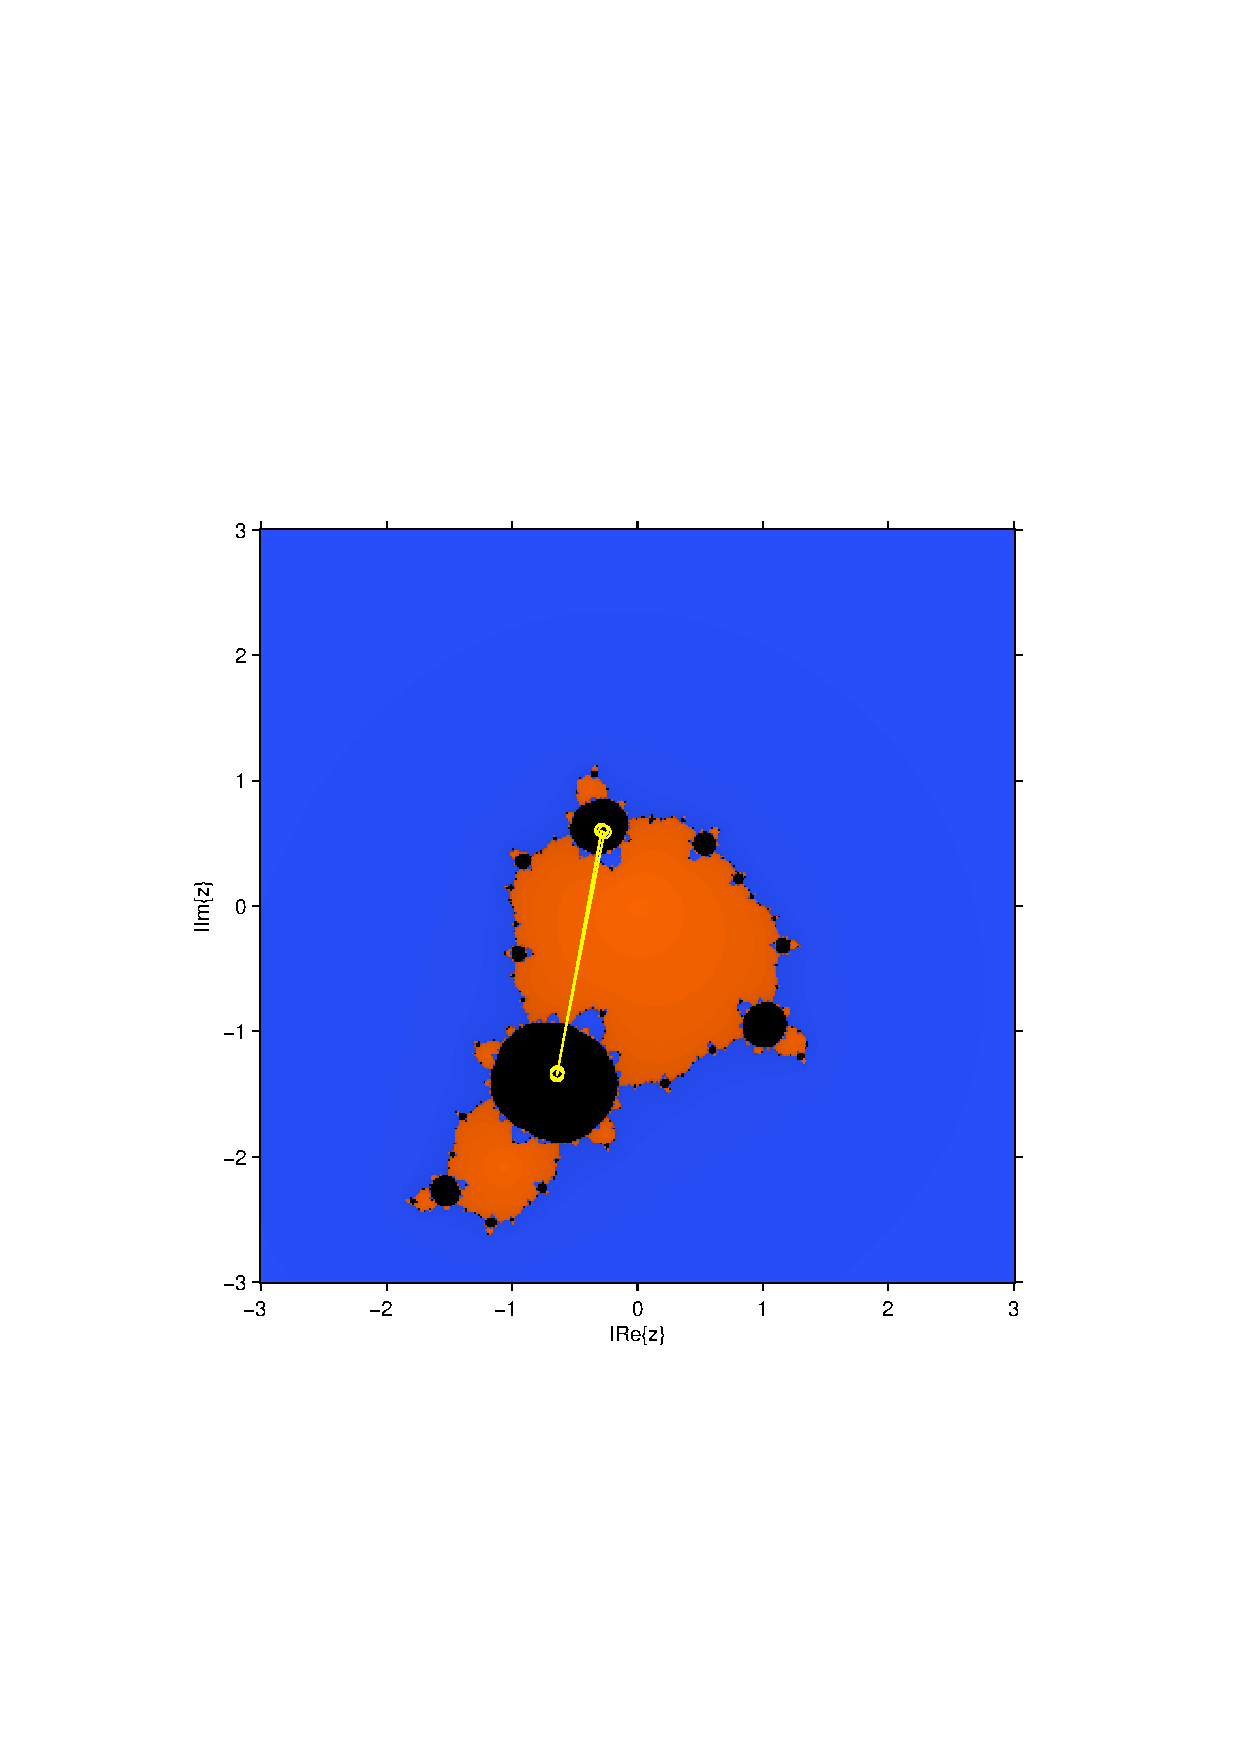
\includegraphics[width=\linewidth]{cardioide.png}
		\caption{Plano dinámico asociado a $\gamma=0.1752+0.4i$}\label{cardioide}
	\end{minipage}
	\begin{minipage}[m]{0.5\linewidth}% \hspace{1cm}
		\centering \includegraphics[width=\linewidth]{rightcircle.png}
		\caption{Plano dinámico asociado a $\gamma=0.283$}\label{rightcircle}
	\end{minipage}
\end{figure}

Otras regiones del plano de parámetros $P_1$ donde hay órbitas atractoras de periodo 2, son aquellas correspondientes a las Figuras \ref{rightcircle} y \ref{circulocardioide}. Nótese que en ésta última (Figura \ref{circulocardioide}) hay dos órbitas de periodo 2 distintas, con un punto crítico libre contenido en cada una de sus cuencas de atracción. Una órbita de periodo 4 es encontrada en el plano dinámico correspondiente a $\gamma=1.24$, como se muestra en la Figura \ref{4periodorbit}, que se corresponde a valores de $\gamma$ contenidos en uno de los conjuntos de Mandelbrot en la izquierda de la antena del plano de parámetros (ver Figura \ref{fig3:c}).

\begin{figure}[h!]
	\subfloat[]{\includegraphics[width=0.50\textwidth]{circlecardioide1.png}}
	\subfloat[]{\includegraphics[width=0.50\textwidth]{circlecardioide2.png}}
	\caption{Planos dinámicos asociados a $\gamma=0.12+0.4i$}\label{circulocardioide}
\end{figure}


\begin{figure}[h!]
	\subfloat[$\gamma=1.24$]{\includegraphics[width=0.50\textwidth]{4periodorbit.png}\label{4periodorbit}}
	\subfloat[$\gamma=0.31$]{\includegraphics[width=0.50\textwidth]{antena.png}\label{antena}}
	\caption{Planos dinámicos para diferentes valores de $\gamma$.}
\end{figure}

Por último, el plano dinámico correspondiente a $\gamma=0.31$ se muestra en la Figura \ref{antena} con el objetivo de ver el comportamiento de la derecha de la antena en $P_1$; incluso este área muestra una muy buena estabilidad del método. 

\section{Conclusiones}

El comportamiento dinámico de la familia \eqref{generalizacion} sobre polinomios cuadráticos es muy rico. Analizando los planos de parámetros, se ha mostrado que algunos valores del parámetro $\gamma$, eso es, miembros de la familia, pueden no converger a las raíces. La existencia de órbitas periódicas de periodo 2 ha sido mostrada, y su expresión analítica ha sido obtenida en términos del parámetro $\gamma$. Sin embargo, es importante recalcar que algunos de las áreas inestables encontradas en $P_1$ se corresponden con valores complejos del parámetro $\gamma$, los cuales son muy raramente usados, y en consecuencia la gran mayoría del plano de parámetros se corresponde con métodos iterativos con un muy buen comportamiento numérico.

\chapter{Discretización de segundo orden de la ecuación de Burgers}\label{articuloburger}

En este capítulo presentamos y aplicamos una alternativa a la discretización implícita tradicional llamada método de Crank-Nicholson, el cual aplicaremos directamente sobre la ecuación no lineal de Burgers (\ref{BE}). Con tal discretización obtendremos un sistema de ecuaciones no lineales (para cada instante) $F(u(x,t_j))=0$, que deberá ser resuelto mediante el uso de método iterativos de punto fijo.
Concretamente usaremos el método clásico de Newton (cuyo orden de convergencia es dos),
\begin{eqnarray} \label{newton}
x^{(k+1)}=x^{(k)}-[F'(x^{(k)})]^{-1}F(x^{(k)}),
\end{eqnarray}
el método de Traub de orden tres (ver \cite{TR})
\begin{eqnarray} \label{traub}
y^{(k)}=x^{(k)}-[F'(x^{(k)})]^{-1}F(x^{(k)}), \\\nonumber
x^{(k+1)}=y^{(k)}-[F'(x^{(k)})]^{-1}F(y^{(k)})
\end{eqnarray}
y el método denotado como M5 (ver \cite{ACT}), de orden de convergencia cinco, cuya expresión iterativa es,
\begin{eqnarray} \label{m5}
y^{(k)}&=&x^{(k)}-[F'(x^{(k)})]^{-1}F(x^{(k)}), \\ \nonumber
z^{(k)}&=&y^{(k)}-5[F'(x^{(k)})]^{-1}F(y^{(k)}), \\
x^{(k+1)}&=&z^{(k)}-\frac{1}{5}
[F'(x^{(k)})]^{-1}[-16F(y^{(k)})+F(z^{(k)})].\nonumber
\end{eqnarray}

La estabilidad del método es analizada numéricamente, comprobando que se trata de un método incondicionalmente estable. El método de Crank-Nicholson presentado tiene una precisión de segundo orden tanto en el espacio como en el tiempo. El método será puesto a prueba mediante el uso de distintos valores de $\varepsilon$ y distintas condiciones iniciales con el objetivo de analizar su estabilidad y consistencia; para llevar esto a cabo, la solución obtenida a partir de los métodos iterativos es comparada entre ellos así como con la solución exacta. Estos resultados, así como sus interesantes conclusiones, fueron presentados en la \textit{``16th Edition of the	Mathematical Modelling Conference Series''} y publicados por la revista \textit{Algorithms 8(2015) 224-233} bajo el título \textit{``Numerical Solution of Turbulence Problems by Solving Burgers’ Equation''} (véase \cite{paperburgers}).

Ahora, consideremos la ecuación en derivadas parciales unidimensional de Burgers (ver \cite{Bateman} y \cite{Burgers}),
\begin{equation}\label{BE}
\frac{\partial u}{\partial t}+u \frac{\partial u}{\partial
	x}=\frac{1}{Re} \frac{\partial^2 u}{\partial^2 x}, \ \ (x,t)\in
\Omega
\end{equation}
donde $\Omega=(a,b)\times(0,T]$. La condición inicial es tal que $u(x,0)=f(x)$, $a<x<b$ y las de contorno son tales que $u(a,t)=g_1(t)$,
$u(b,t)=g_2(t)$, $0\leq t \leq T$; siendo $Re$ el número de Reynolds 
y $f$, $g_1$ y $g_2$ unas funciones dadas suficientemente suaves. Por simplicidad, algunas veces usaremos $\varepsilon$ en vez de $\frac{1}{Re}$.

La ecuación de Burgers es usada para la descripción de problemas de turbulencia, en la teoría de las ondas sísmicas y en procesos estocásticos continuos. Tiene aplicaciones en dinámica de gases, conducción del calor y elasticidad, entre otras.

Este problema muestra una estructura bastante similar a la de las ecuaciones de Navier-Stokes, debido a la forma del término no lineal de convección y la existencia del término correspondiente a la viscosidad. Así pues, éste puede ser considerado como una forma simplificada de la ecuación de Navier-Stokes. En estos últimos años, diversos investigadores han usado distintos métodos numéricos, especialmente basados en diferencias finitas, técnicas de frontera de elementos finitos y métodos variacionales, con el objetivo de resolver este problema (ver, por ejemplo, \cite{KA,HSH,WT} y las referencias que se citan en su interior).

Además, la ecuación no lineal de Burgers \eqref{BE} es una de las pocas ecuaciones en derivadas parciales no lineal cuya solución puede ser obtenida analíticamente de forma exacta para una función inicial arbitraria $f(x)$. La denominada transformación de Hopf-Cole \cite{H-C}
\begin{equation}\label{transformation}
u(x,t)=-\left( \frac{2}{Re} \right) \frac{\phi_x(x,t)}{\phi(x,t)},
\end{equation}
facilita dicha resolución, siendo $\phi$ la solución a la ecuación lineal de difusión
\begin{equation}\label{ecdiffusion}
\frac{\partial \phi(x,t)}{\partial t}=\frac{1}{Re} \frac{\partial^2
	u}{\partial^2 x}.
\end{equation}
Siendo $u$ la solución de la ecuación de Burgers (\ref{BE}). Esta transformación nos permite obtener los valores exactos de $u(x,t)$ porque la ecuación (\ref{ecdiffusion}) tiene una solución en series de Fourier, sin embargo, su coste computacional es muy elevado y por eso nosotros sólo la usamos para comparar la precisión de nuestros resultados (como veremos un poco más adelante, las integrales de los coeficientes de Fourier deben ser calculadas). Como podemos ver en \cite{KA}, algunos investigadores han aprovechado esta transformación y han aplicado el método de Crank-Nicholson sobre la ecuación lineal (\ref{ecdiffusion}) con el objetivo de obtener en primer lugar los valores de $\phi(x,t)$ y posteriormente los de $u(x,t)$. Otros autores han usado el método implícito, donde $\frac{\partial u}{\partial t}$ es aproximado por diferencias finitas regresivas, sin embargo debido a que su error de truncamiento es de orden uno, la precisión de los resultados decrece.

La forma más fácil de discretizar un problema de ecuaciones en derivadas parciales (como el que tenemos en la ecuación (\ref{BE})) consiste en reducir el dominio continuo a un número finito de puntos equiespaciados $(x_i,t_j)$, localizados en los nodos de un mallado rectangular uniforme. Así pues, ahora las derivadas parciales de $u$ pueden ser aproximadas por los siguientes cocientes de diferencias 
\begin{equation} \label{forward}
\frac{\partial u(x_i,t_j)}{\partial x}\approx\frac{u_{i+1,j}-u_{i,j}}{h}, \qquad\frac{\partial u(x_i,t_j)}{\partial t}\approx\frac{u_{i,j+1}-u_{i,j}}{k}
\end{equation}
las cuales son llamadas diferencias progresivas, y tienen un error de truncamiento de orden 1. Las derivadas parciales de $u$ también pueden ser obtenidas a partir de
\begin{equation} \label{backward}
\frac{\partial u(x_i,t_j)}{\partial x}\approx\frac{u_{i,j}-u_{i-1,j}}{h}, \qquad\frac{\partial u(x_i,t_j)}{\partial t}\approx\frac{u_{i,j}-u_{i,j-1}}{k},
\end{equation}
las cuales son llamadas diferencias regresivas, y también tienen un error de truncamiento de orden 1. Finalmente, las derivadas parciales de $u$ también pueden ser obtenidas a partir de
\begin{equation} \label{central}
\frac{\partial u(x_i,t_j)}{\partial x}\approx\frac{u_{i+1,j}-u_{i-1,j}}{2h}, \qquad\frac{\partial u(x_i,t_j)}{\partial t}\approx\frac{u_{i,j+1}-u_{i,j-1}}{2k},
\end{equation}
\begin{equation} \label{centralsecond}
\frac{\partial^2 u(x_i,t_j)}{\partial x^2}\approx\frac{u_{i+1,j}-2u_{i,j}+u_{i-1,j}}{h^2}, \qquad\frac{\partial^2 u(x_i,t_j)}{\partial t^2}\approx\frac{u_{i,j+1}-2u_{i,j}+u_{i,j-1}}{k^2},
\end{equation}
las cuales son llamadas diferencias centrales, y tienen un error de truncamiento de orden 2. En estas expresiones, $u_{i,j}$ denota el valor aproximado de la función incógnita $u$ en $(x_i,t_j)$, $h=\frac{b-a}{n}$, y $k=\frac{T-0}{m}$ son, respectivamente, el paso en el espacio y el tiempo del mallado, y $n$ y $m$ son, respectivamente, la cantidad de subintervalos considerados en el dominio del espacio y del tiempo. Así pues, tenemos que $x_{i+1}=x_i+h$ y $t_{j+1}=t_j+k$, donde $i=0,1,...,n-1$ y
$j=0,1,...,m-1$.

Apliquemos ahora el esquema en diferencias de Crank-Nicholson, el cual consiste en discretizar la ecuación (\ref{BE}) en dos instantes de tiempo consecutivos y promediarlos. En el primer instante $t_j$, aproximamos $\frac{\partial u}{\partial t}$ por las diferencias progresivas descritas en la ecuación (\ref{forward}), y en el segundo instante $t_{j+1}$, lo hacemos por las regresivas. En ambos instantes aproximamos $\frac{\partial u}{\partial x}$ y $\frac{\partial^2u}{\partial x^2}$  por las diferencias centrales (descritas en las ecuaciones (\ref{central}) y (\ref{centralsecond}), respectivamente). Por medio de este procedimiento obtenemos, para el primer instante,
\begin{equation} \label{firstinstant}
\frac{u_{i,j+1}-u_{i,j}}{k}-\varepsilon\frac{u_{i+1,j}-2u_{i,j}+u_{i-1,j}}{h^2}+u_{i,j}\frac{u_{i+1,j}-u_{i-1,j}}{2h}=0
\end{equation}
y para el segundo,
\begin{equation} \label{secondinstant}
\frac{u_{i,j+1}-u_{i,j}}{k}-\varepsilon\frac{u_{i+1,j+1}-2u_{i,j+1}+u_{i-1,j+1}}{h^2}+u_{i,j+1}\frac{u_{i+1,j+1}-u_{i-1,j+1}}{2h}=0.
\end{equation}
Después de promediar ambas expresiones, resulta
\begin{eqnarray} \label{average}
Bu_{i,j+1}u_{i+1,j+1}-Bu_{i,j+1}u_{i-1,j+1}-Cu_{i+1,j+1}+2Cu_{i,j+1}-Cu_{i-1,j+1}+Au_{i,j+1}=\\\nonumber Cu_{i+1,j}+(A-2C)u_{i,j}+Cu_{i-1,j}+Bu_{i,j}u_{i+1,j}-Bu_{i,j}u_{i-1,j}
\end{eqnarray}
donde $A=\frac{1}{k}$, $B=\frac{1}{4h}$,
$C=\frac{\varepsilon}{2h^2}$ y el rango de índices es
$i=1,...,n-1$ y $j=0,1,...,m-1$. Esta expresión (la cual tiene un error de truncamiento de orden 2) resulta en $m$ sistemas no lineales de $n-1$ incógnitas y $n-1$ ecuaciones. Cada uno de estos sistemas aparece tras considerar que ya conocemos de antemano el valor de $u_{0,j}$ y	$u_{n,j}$, $\forall j$ (de las condiciones de contorno) y $u_{i,0}$,
$\forall i$ de la condición inicial. Nótese que los valores correspondientes al subíndice $j$ han sido calculados en el sistema previo al actual, y que las únicas incógnitas serán aquellas con el subíndice $j+1$.

\section{Resultados numéricos}
Comparemos pues, nuestros resultados con los de la solución exacta, la cual puede ser obtenida mendiante la transformación de Hopf-Cole mencionada en las ecuaciones 	(\ref{transformation}) y (\ref{ecdiffusion}). Para ello, primero calculamos
\[
\phi(x,t)=A_0+\sum\limits_{p=1}^\infty
A_pe^{-p^2\varepsilon\pi^2t}\cos{(p\pi x)}
\]
y posteriormente, a partir de la ecuación (\ref{transformation}), obtenemos
\begin{equation}\label{uanalitica}
u(x,t)=2\pi\varepsilon\frac{\sum_{p=1}^\infty
	A_pe^{-p^2\varepsilon\pi^2t} p\ \ \sin{(p\pi
		x)}}{A_0+\sum_{p=1}^\infty A_pe^{-p^2\varepsilon\pi^2t}\cos{(p\pi
		x)}}
\end{equation}
donde
\[
A_0=\int_{a}^{b} e^{-\frac{1}{2\varepsilon}\int_{a}^{x} u(\xi,0)d\xi} dx,
\]
\[
A_p=2\int_{a}^{b} e^{-\frac{1}{2\varepsilon}\int_{a}^{x}
	u(\xi,0)d\xi} \cos{(p\pi x)}dx, \ \ p=1,2,\ldots
\]
Nuestro objetivo, para poder demostrar la precisión de nuestros resultados, es obtener por lo menos cinco decimales exactos de la solución, y para ello hemos observado que es suficiente con coger tan sólo dos sumandos de la serie de Fourier. Así pues, sólo tenemos que calcular $A_0$, $A_1$ y $A_2$. Dichos coeficientes son calculados en formato \textit{long} mediante la función \textit{int(integrando,limite\_inferior,limite\_superior)} de Matlab.

En los ejemplos mostrados a continuación, consideramos que las condiciones de contorno son cero, así pues \mbox{$g_1(t)=0$} y $g_2(t)=0$, lo que significa que $u_{0,j}=0$ y $u_{n,j}=0$, $\forall j$. En este caso podemos comparar nuestros resultados con la solución exacta, sin embargo nuestro método ha resultado ser incondicionalmente estable, numéricamente hablando, para todas las condiciones de contorno utilizadas. Para la obtención de ambas soluciones, la exacta y la aproximada, se ha usado la versión R2013a de Matlab, con doble precisión. El criterio de parada usado es
$$\|u^{(k+1)}(x,t_j)-u^{(k)}(x,t_j)\|+\|F(u^{(k+1)}(x,t_j))|<10^{-15}$$.
%\vspace{0.5 cm}
\textbf{Ejemplo 1.} Las condiciones iniciales y de contorno de la ecuación de Burgers para este ejemplo son
\[
u(x,0)=\frac{2\varepsilon \beta \pi sin(\pi x)}{\alpha+\beta cos(\pi x)}, \qquad 0\le x\le 2
\]
y $u(0,t)=u(2,t)=0, t\ge 0$ donde $\alpha=5$ y $\beta=4$.
\vspace{0.25 cm}

En las Tablas \ref{compn} a \ref{compe} se muestra, para distintos valores de $n$, $m$
y $\varepsilon$, el número medio de iteraciones requeridas al usar los métodos de Newton, Traub y M5. También mostramos el error máximo, EM, que se obtiene para cada valor de $x_i$ y $t_j$, donde $i=0,1,...,n-1$ y $j=0,1,...,m-1$. La aproximación inicial de cada sistema no lineal a resolver es la solución del anterior (y para el primer sistema, la aproximación inicial es el valor exacto de la condición inicial). A continuación obtenemos la matriz de errores como la diferencia absoluta entre la solución aproximada y la solución exacta en cada nodo, finalmente llamamos el error máximo al mayor elemento de esa matriz. Mientras que otros autores prefieren comparar y dar el valor del error sólo en algunos puntos del mallado, nosotros hemos preferido un criterio más riguroso, éste consiste en comparar todos los valores del error de la matriz de errores y dar el valor del EM, de esta forma nos hacemos una mejor idea sobre cómo de mala es la peor situación posible, y sabemos con toda seguridad que el error del resto de puntos será siempre inferior a este EM; de la otra forma no podemos saber si realmente existe algún otro punto cuyo error sea mayor.

Un resultado interesante se desprende de la matriz de errores cuando el tiempo de observación es suficientemente grande, lo cual se puede conseguir mediante una rápida atenuación (valores grandes de $\varepsilon$) o mediante un largo tiempo de estudio (valores grandes de $T$). Si obtenemos el EM entre todos los valores de $x$ para cada tiempo, observamos que el EM se incrementa muy deprisa al principio pero que una vez se alcanza el máximo, éste empieza a decrecer. Este resultado se puede ver en la Figura \ref{atenuaciones}.

En la Tabla \ref{compn} establecemos el tiempo máximo de estudio, la cantidad de nodos en el tiempo y la constante de Reynolds, como $t_{max}=1$,
$m=100$ y $\varepsilon =\frac{1}{Re}=0.1$, y variamos la cantidad de nodos espaciales. Para cada caso obtenemos el ya mencionado EM y el número medio de iteraciones ($\bar{K}$) requeridas para resolver cada sistema no lineal mediante el uso del método de Newton, Traub y M5. De estos resultados observamos que, en general, cuantos más subintervalos espaciales cojamos (paso espacial más pequeño), menor es el EM.

En la Tabla \ref{compm} repetimos el mismo proceso, pero en este caso fijamos la cantidad de nodos en el espacio y variamos la cantidad de nodos en el tiempo. Así pues, $t_{max}=1$, $n=100$ y $\varepsilon =\frac{1}{Re}=0.1$. Como podemos observar, en un primer momento parece que cuantos más subintervalos en el tiempo cojamos, menor es el EM (de forma similar a como pasó con la Tabla \ref{compn}, donde probamos cantidades distintas de subintervalos en el espacio), sin embargo existe un límite a partir del cual el error empieza a incrementarse de nuevo. Para este caso, el error mínimo es obtenido con $m=20$.

\begin{figure}[h!]
	\centering
	\subfloat[$\varepsilon =1$]{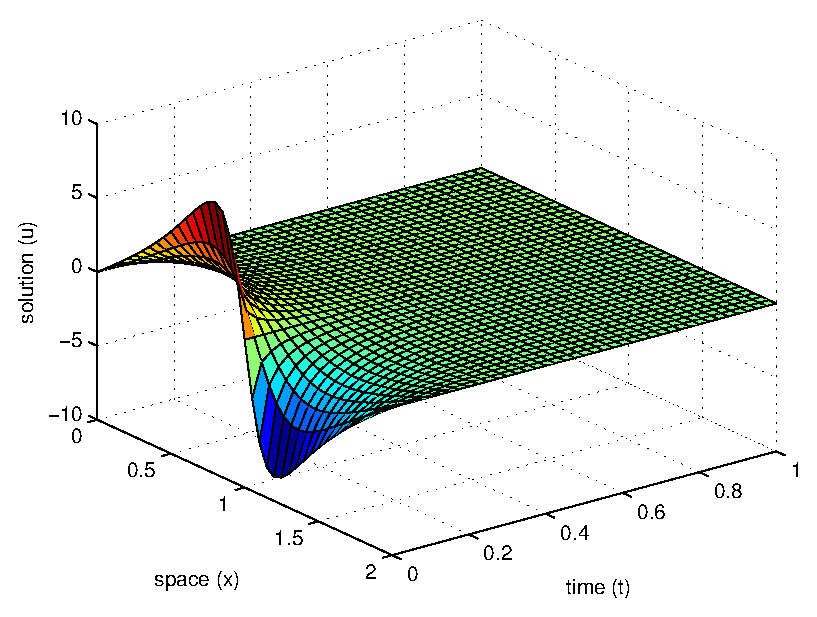
\includegraphics[width=0.33\textwidth]{uepsilon1.eps}} %\hspace{0.5cm}
	\subfloat[$\varepsilon =0.1$]{\includegraphics[width=0.33\textwidth]{uepsilon01.eps}} %\hspace{0.5cm}
	\subfloat[$\varepsilon =0.005$]{\includegraphics[width=0.33\textwidth]{uepsilon0005.eps}} \\
	\subfloat[$\varepsilon =1$]{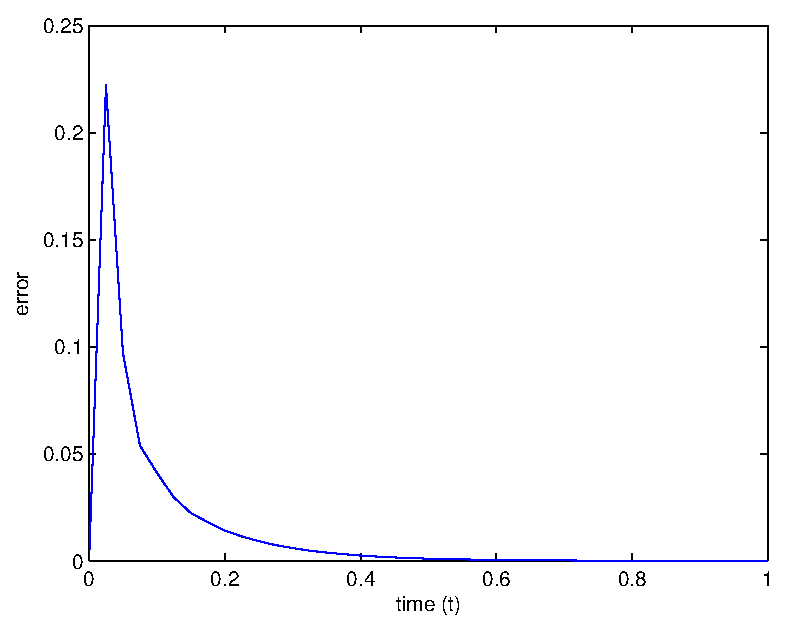
\includegraphics[width=0.33\textwidth]{errorepsilon1.eps}} %\hspace{0.5cm}
	\subfloat[$\varepsilon =0.1$]{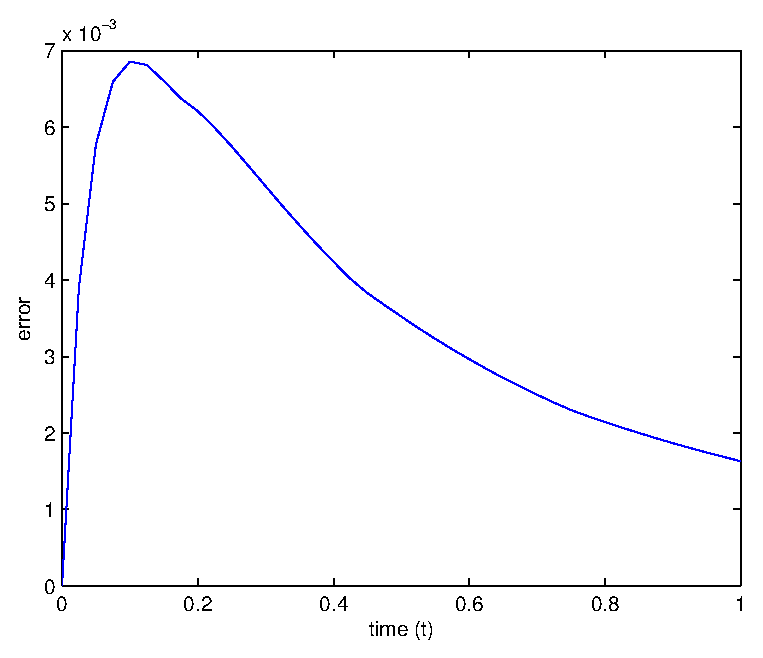
\includegraphics[width=0.33\textwidth]{errorepsilon01.eps}} %\hspace{0.5cm}
	\subfloat[$\varepsilon =0.005$]{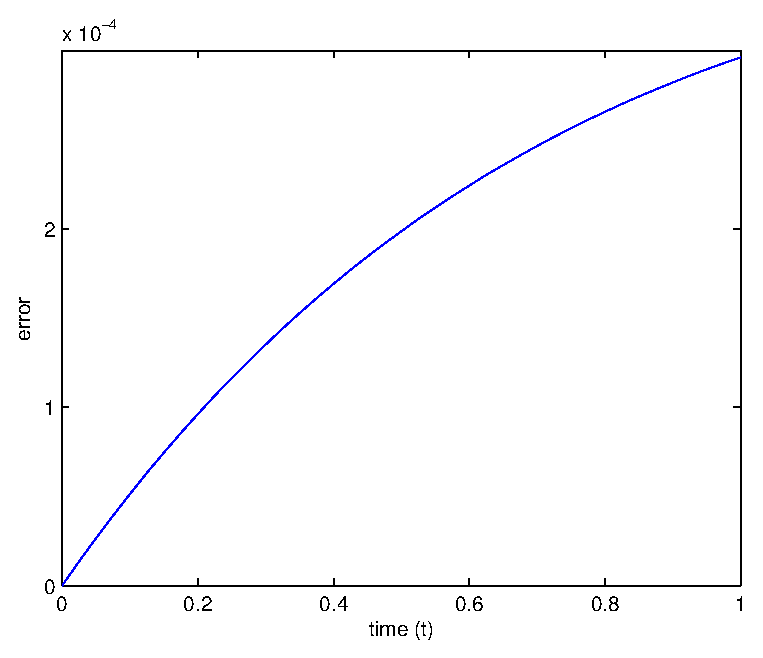
\includegraphics[width=0.33\textwidth]{errorepsilon0005.eps}} \vspace{6pt}
	\caption{Solución aproximada y curva de la progresión del error máximo para distintos tiempos y valores de $\varepsilon$, con \mbox{$n=m=40$} y $t_{max}=1$.}
	\label{atenuaciones}
\end{figure}

%\vspace{-12pt}
\begin{table}[h!]
	\centering
	\small
	\begin{tabular}{cccccc}
		\toprule
		&\boldmath $n=10$ &\boldmath $n=20$ &\boldmath $n=40$ &\boldmath $n=80$ &\boldmath $n=160$ \\ \midrule
		\multicolumn{1}{c}{Error máximo}    & 0.09033    &  0.029932   &  0.0070658   & 0.0017149   &   0.00039376   \\
		\multicolumn{1}{c}{$\bar{K}_N$} &  4   &  4   &   4  &  4   &  4    \\
		\multicolumn{1}{c}{$\bar{K}_T$}  &  3   &   3  &   3  &   3  &   3   \\
		\multicolumn{1}{c}{$\bar{K}_{M5}$}     &  3    &  3   &  3   &  3   &   3   \\ \bottomrule
	\end{tabular}
	\caption{Comparación del EM (error máximo) y las iteraciones por método, para distintas cantidades de subintervalos en el espacio.}\label{compn}
\end{table}

\begin{table}[h!]
	\centering
	\small
	\begin{tabular}{cccccc}
		\toprule
		&\boldmath $m=10$ &\boldmath $m=20$ &\boldmath $m=40$ &\boldmath $m=80$ &\boldmath $m=160$ \\ \midrule
		\multicolumn{1}{c}{Error máximo}    & 0.0043069    &  0.00015291   & 0.00083542   & 0.0010565  & 0.0011128    \\
		\multicolumn{1}{c}{$\bar{K}_{N}$} &  4.4  & 4.15  & 4   &   4 &  4   \\
		\multicolumn{1}{c}{$\bar{K}_{T}$}  &  3.4  &  3.1  &  3  &  3  &  3   \\
		\multicolumn{1}{c}{$\bar{K}_{M5}$}     &  3    &   3   &  3  &  3  &  3   \\ \bottomrule
	\end{tabular}
	\caption{Comparación del EM (error máximo) y las iteraciones por método, para distintas cantidades de subintervalos en el tiempo.}\label{compm}
\end{table}

En la Tabla \ref{compe} repetimos nuevamente el proceso, sin embargo esta vez estudiamos el efecto de escoger un valor pequeño, normal o grande de la constante de Reynolds ($Re$); aunque en verdad usamos $\varepsilon=\frac{1}{Re}$, por simplicidad. Para ello fijamos la cantidad de nodos en el espacio y el tiempo, así como el tiempo máximo de estudio. De esta forma tenemos que $t_{max}=1$,	$n=40$ y $m=40$.

\begin{table}[h!]
	\centering
	\small
	\begin{tabular}{cccccccc}
		\toprule
		&\boldmath $\varepsilon = 1$ &\boldmath $\varepsilon = 0.1$ &\boldmath $\varepsilon = 0.05$ &\boldmath $\varepsilon = 0.03$ &\boldmath $\varepsilon = 0.02$ &\boldmath $\varepsilon = 0.01$ &\boldmath $\varepsilon = 0.005$ \\ \midrule
		\multicolumn{1}{c}{Error máximo}    & 0.22216 & 0.0068572 & 0.0035207 & 0.0021242 & 0.0014188 & 0.000708 & 0.000296 \\
		\multicolumn{1}{c}{$\bar{K}_{N}$} & 3.9 & 4 & 4 & 4 & 4 & 3.85 & 3 \\
		\multicolumn{1}{c}{$\bar{K}_{T}$}  & 3.15 & 3 & 3 & 3 & 3 & 3 & 3 \\
		\multicolumn{1}{c}{$\bar{K}_{M5}$}     & 2.8 & 3 & 3 & 3 & 3 & 3 & 2 \\ \bottomrule
	\end{tabular}
	\caption{Comparación del EM y las iteraciones por método, para distintos valores de $\varepsilon$.}\label{compe}
\end{table}

Es importante recalcar que el valor máximo de $\varepsilon$ que se puede usar para mantener el método funcionando debidamente dependerá de la cantidad de subintervalos que cojamos, esto ocurre debido a que como mayor es la atenuación, más abruptas son las curvas en el eje del tiempo. Para mantener un error pequeño se requiere un mallado más fino, lo cual se puede obtener incrementando la cantidad de subintervalos en el tiempo. En la Tabla \ref{compe} podemos ver numéricamente este fenómeno. Para una rápida atenuación ($\varepsilon = 1$) el error es bastante grande debido a que la curva es muy abrupta (como hemos dicho podríamos reducir el error de este caso tomando más subintervalos en el tiempo), sin embargo cuanto más lenta es la atenuación (valores bajos de $\varepsilon$), más bajo es el EM. Si seguimos cogiendo valores bajos de atenuación ($\varepsilon$ pequeña), el pico de la curva característica del EM no será alcanzado, y en consecuencia el EM será incluso más pequeño (para este ejemplo ésto sucede para $\varepsilon = 0.01$ e incluso más para $\varepsilon = 0.005$). Véase la Figura \ref{atenuaciones} para una mejor comprensión de estas diferentes situaciones.

De las Tablas \ref{compn} a la \ref{compe} se desprenden algunas conclusiones: usar un método de orden más alto (como el M5) no representa una mayor ventaja comparado con un método típico de orden tres (como el de Traub), sin embargo sí existe una diferencia significante entre usar un método de tercer orden y uno típico de segundo (como el de Newton). Cuantos más subintervalos en el espacio cojamos, menor es el EM; sin embargo, esto no ocurre con la cantidad de subintervalos en el tiempo, lo cual significa que hay una cantidad óptima de subintervalos en el tiempo que reduce el EM hasta su mínimo, pero pasado éste el error empieza a incrementarse de nuevo, y el incremento del coste computacional (debido al incremento de operaciones en coma flotante, tiempo de ejecución, etc.) de tener que resolver tantos sistemas no conlleva ninguna ventaja. Tal y como hemos visto en la Tabla \ref{compe}, si queremos estudiar una situación con una gran atenuación ($Re$ pequeño), necesitaremos una cantidad más elevada de subintervalos en el tiempo, comparado con aquellas situaciones donde la atenuación es menor (esto significa que el coste computacional de tener que resolver más sistemas no lineales será mayor), sin embargo en este caso tomar más subintervalos en el espacio no resuelve el problema.
\vspace{0.5 cm} \\
\textbf{Ejemplo 2.} Consideremos ahora las siguientes condiciones iniciales y de contorno para la ecuación de Burgers
\begin{eqnarray}
u(x,0)=\left\{ \begin{array} {ll}
\sin(\pi x),             & 0< x \leq 1 \\
-\frac{1}{2}\sin(\pi x), & 1< x \leq 2 \\
0& 2< x\leq 5
\end{array} \right.
\end{eqnarray}
y $u(0,t)=u(5,t)=0, t\ge 0$.
\vspace{0.25 cm}

En la Figura \ref{mittal} vemos un gráfico de la solución aproximada obtenida con nuestro método en distintos instantes, para $0\leq x\leq 5$ y para distintos valores de  $\varepsilon$, y en la Tabla \ref{example2table} mostramos los resultados numéricos de esta solución para algunos valores de $x, t$ y $\varepsilon$.

\begin{figure}[h!]
	\centering
	\subfloat[]{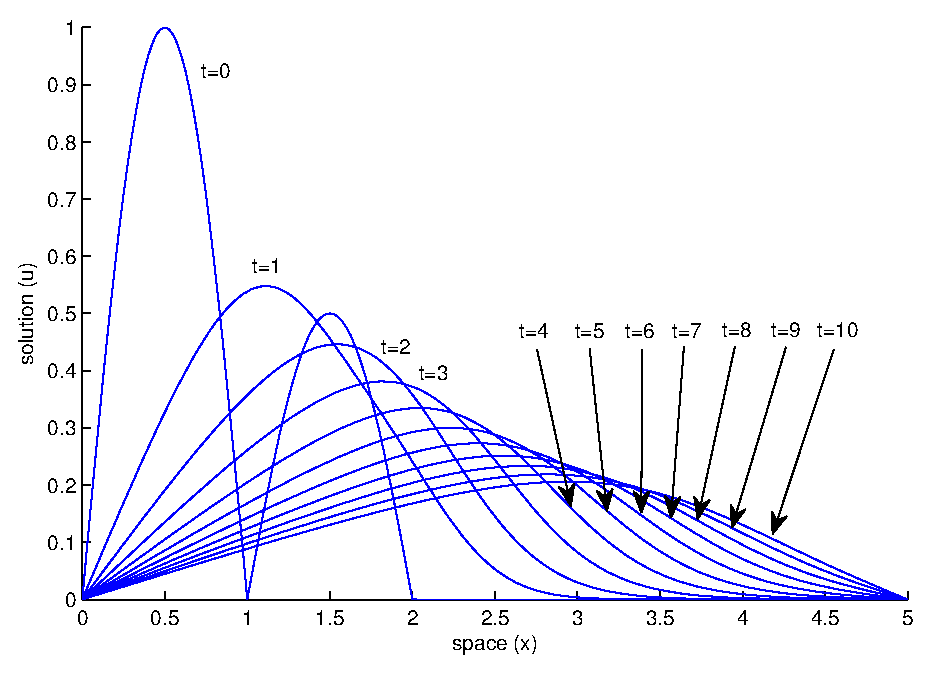
\includegraphics[width=0.50\textwidth]{example2epsilon01.eps}} %\hspace{0.5cm}
	\subfloat[]{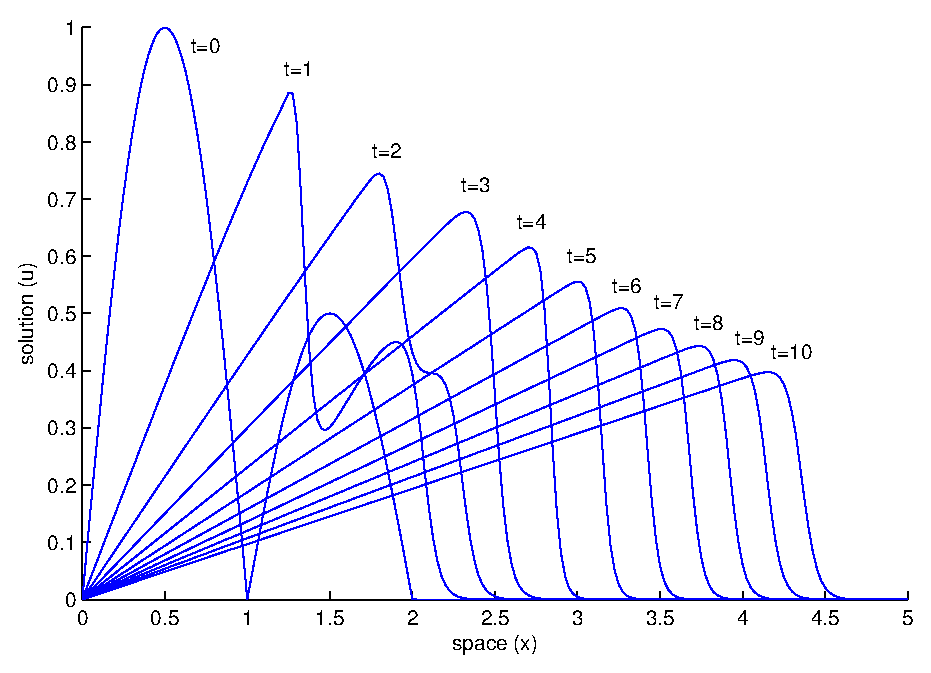
\includegraphics[width=0.50\textwidth]{example2epsilon001.eps}}
	\caption{Solución para distintos instantes y valores de $\varepsilon$, ambos con $n=m=200$ y $t_{max}=10$. (\textbf{a}) $\varepsilon =0.1$;  (\textbf{b}) $\varepsilon =0.01$.}
	\label{mittal}
\end{figure}

\vspace{-12pt}
\begin{table}[h!]
	\small
	\centering
	\begin{tabular}{cccc}
		\toprule
		\boldmath $x$   &\boldmath $t$  &\boldmath $\varepsilon =0.1$ &\boldmath $\varepsilon =0.01$ \\
		\midrule
		1.5 & 2  &  0.44533     &  0.63548                          \\
		& 4  &  0.28961     &  0.34573                          \\
		& 6  &  0.20701     &  0.23678                          \\
		& 8  &  0.16020     &  0.17999                          \\
		& 10 &  0.13041     &  0.14516                          \\
		\hline
		3   & 2  &  0.02972     &  0.00000                          \\
		& 4  &  0.14900     &  0.00470                          \\
		& 6  &  0.22312     &  0.47269                          \\
		& 8  &  0.22501     &  0.35971                          \\
		& 10 &  0.20562     &  0.29021                          \\
		\hline
		4.5 & 2  &  0.00001     &  0.00000                          \\
		& 4  &  0.00145     &  0.00000                          \\
		& 6  &  0.01171     &  0.00000                          \\
		& 8  &  0.03557     &  0.00000                          \\
		& 10 &  0.06242     &  0.02066                          \\
		\bottomrule
	\end{tabular}
	\caption{Resultados numéricos de la solución aproximada para distintos valores de $x, t$ y $\varepsilon$.}\label{example2table}
\end{table}

Estos resultados son muy similares a aquellos obtenidos por Mittal y Singhal en \cite{MS}, donde transforman la ecuación de Burgers en un sistema de ecuaciones diferenciales ordinarias no lineales y posteriormente lo resuelven mediante el método de segundo orden de Runge-Kutta-Chebyshev. Aunque las técnicas usadas para resolver el problema son diferentes, los resultados obtenidos por Mittal-Singhal y los nuestros, mostrados en la Tabla \ref{example2table} y en la Figura \ref{mittal}, son del mismo orden de magnitud. Como podemos ver en la Figura \ref{mittal}, ocurre efectivamente, que cuanto más pequeño es $\varepsilon$, más lenta es la atenuación. Aunque en este ejemplo hemos usado una condición inicial definida a trozos, y normalmente éstas siempre traen más problemas, nuestros resultados obtenidos han sido satisfactorios. Dado que hemos considerado un límite del tiempo de estudio bastante elevado ($t=10$), hemos tenido que coger un valor de $m$ más grande con el objetivo de mantener un buen tamaño de mallado. Los resultados mostrados tanto en la Figura \ref{mittal} como en la Tabla \ref{example2table} son los mismos tanto si usamos el método de Newton, como el de Traub o como el de M5.

\section{Conclusiones}

Como hemos visto en los Ejemplos 1 y 2, nuestro método tiene la misma precisión que aquellos métodos que aplican la transformación de Hopf-Cole o Runge-Kutta al sistema de ecuaciones diferenciales equivalente. Nuestro método es mucho más directo, dado que no requiere la aplicación de la mencionada transformación.

También hemos aprovechado los resultados numéricos para sacar algunas conclusiones acerca de la importancia de la cantidad de subintervalos en el espacio y en el tiempo para la obtención del mallado sobre el que calculamos la solución, así como la dependencia entre el error y el valor de la constante de Reynolds: si queremos reducir el error, podemos tomar más subintervalos en el espacio, aunque el coste computacional se incrementará debido a que entonces habrá más incógnitas a resolver por sistema. Otra forma de reducir el error es cogiendo más subintervalos en el tiempo, sin embargo hemos visto que hay un límite a partir del cual si seguimos cogiendo mayores valores de $m$, el error se incrementará de nuevo. Al mismo tiempo, tomar más subintervalos en el tiempo también significa incrementar el coste computacional, ya que entonces habrá más sistemas a resolver. También hemos visto que coger mayores valores de atenuación ($\varepsilon$) implica un mayor error debido a que como más rápida es la atenuación, más abrupta es la curva y peor es la aproximación; para solucionar esto, se deberían tomar más subintervalos en el tiempo, aunque no hay necesidad de tomar más subintervalos en el espacio.

% -----------------------------------------------------------------------------------------------------------------
%\newpage
%\thispagestyle{empty}
%\rule{\linewidth}{2pt}
\chapter{Sistemas de ecuaciones no lineales}\label{capitulosistemas}

\section{Nueva familia de métodos de orden cuatro}\label{seccionlichensistemas}

Iniciamos este capítulo retomando la familia de métodos iterativos de orden 4, introducida en la Sección \ref{seccionlichen}, para resolver sistemas no lineales $F(x)=0$, probando su orden de convergencia local y aplicándola a la resolución numérica de la ecuación de Burgers (ya mencionada en el anterior capítulo). Recordemos que su expresión iterativa es

\begin{eqnarray}\label{s1}
y^{(k)} &=& x^{(k)} - \frac{2}{3}[F'(x^{(k)})]^{-1}F(x^{(k)}),\nonumber\\
x^{(k + 1)}& =& x^{(k)} - \left(I - \frac{3}{4}A^{-1}
B\right)[F'(x^{(k)})]^{-1}F(x^{(k)}),
\end{eqnarray}
donde $u ^{(k)} = [F'(x^{(k)})]^{-1}\left(F'(y^{(k)}) -
F'(x^{(k)})\right)$, $A= I + (\frac{3}{2} + \beta )u^{(k)}$,
$B=u^{(k)} + \beta u^{(k)^2}$ y $\beta$ es un parámetro arbitrario.

\subsection{Orden de convergencia}
\begin{theorem}
	Sea\ $\alpha\in D$  el cero de una función suficientemente diferenciable $F:D \in \mathbb{R}^n \rightarrow \mathbb{R}^n$, $n\geq 1$,
	en un conjunto convexo $D$ con una matriz Jacobiana no singular $F'(x)$ en $\alpha$, y sea también $x^{(0)}$ una aproximación inicial lo suficientemente cerca de la raiz $\alpha$.
	Para cualquier valor real del parámetro $\beta$, el esquema definido en
	(\ref{s1}) tiene orden de convergencia cuatro, y cuya ecuación del error está dada por
	\begin{equation*}%\label{2}
	e^{(k + 1)} = \left( \left(1 - \frac{8}{3}\beta\right)I  - {C_3}{C_2} +
	\frac{1}{9}{C_4}\right) e^{(k)^4} + O(e^{(k)^5}),
	\end{equation*}
	donde $C_j = \frac{1}{j!}[F'(\alpha )]^{ - 1}F^{(j)}(\alpha )$, $j =
	2,3,\ldots$ y ${e^{(k)}} = x^{(k)} - \alpha$.
\end{theorem}

\begin{proof}
	Si usamos el desarrollo en series de Taylor de $F\left(x^{(k)}\right)$ y $F'\left(x^{(k)}\right)$ alrededor de $\alpha$, obtenemos
	\begin{equation*}%\label{3}
	F({x^{(k)}}) = {F'}(\alpha )({e^{(k)}} + {C_2}{e^{(k)}}^2 +
	{C_3}{e^{(k)}}^3 + {C_4}{e^{(k)}}^4  + O({e^{(k)}}^5)
	\end{equation*}
	y
	\begin{equation}\label{4}
	{F'}({x^{(k)}}) = {F'}(\alpha )(I + 2{C_2}{e^{(k)}} +
	3{C_3}{e^{(k)}}^2 + 4{C_4}{e^{(k)}}^3  + O({e^{(k)}}^4)).
	\end{equation}\\
	Forzando $[{F'}({x^{(k)}})]^{ -
		1}{F'}({x^{(k)}})={F'}({x^{(k)}})[{F'}({x^{(k)}})]^{ - 1}=I$, obtenemos
	\begin{equation*}%\label{5}
	{[{F'}({x^{(k)}})]^{ - 1}} = (I + {X_2}{e^{(k)}} + {X_3}{e^{(k)}}^2
	+ {X_4}{e^{(k)}}^3  + O({e^{(k)}}^4) ){[{F'}(\alpha )]^{ - 1}},
	\end{equation*}
	donde $X_1=I$ y ${X_m} = -\sum_{j=2}^{m}{j X_{m-j+1}C_j}$,
	$m=2,3,\ldots$. Así pues, la expresión del error en el primer paso del método es
	\begin{equation*}%\label{7}
	\begin{split}
	{y^{(k)}} - \alpha &= \frac{1}{3}{e^{(k)}} +
	\frac{2}{3}{C_2}{e^{(k)}}^2 - \frac{4}{3}(C_2^2 - {C_3}){e^{(k)}}^3
	+ \frac{2}{3}(4C_2^3 - 4{C_2}{C_3} - 3{C_3}{C_2} +
	3{C_4}){e^{(k)}}^4 + O({e^{(k)}}^5).
	\end{split}
	\end{equation*}
	Además,
	\begin{equation}\label{9}
	{F'}({y^{(k)}}) = {F'}(\alpha )\left( I + \frac{2}{3}{C_2}{e^{(k)}}
	+\frac{4}{3}C_2^2 + \frac{1}{3}{C_3}{e^{(k)}}^2 + {Y_4}{e^{(k)}}^3
	+ O({e^{(k)}}^4) \right),
	\end{equation}
	donde ${Y_4} =  - \frac{8}{3}C_2^3 + \frac{8}{3}{C_2}{C_3} +
	\frac{4}{3}{C_3}{C_2} + \frac{4}{{27}}{C_4}$.
	
	
	Ahora, obtenemos el desarrollo de Taylor de ${u^{(k)}}$ a partir de \eqref{4} y	\eqref{9}:
	\begin{equation*}%\label{10}
	\begin{split}
	{u^{(k)}}
	&= {[{F'}({x^{(k)}})]^{ - 1}}[{F'}({y^{(k)}}) - {F'}({x^{(k)}})]\\
	&=- \frac{4}{3}{C_2}{e^{(k)}} + 4C_2^2 - \frac{8}{3}{C_3}{e^{(k)}}^2
	+ - \frac{{32}}{3}C_2^3 + 8{C_2}{C_3}+ \frac{{16}}{3}{C_3}{C_2} -
	\frac{{104}}{{27}}{C_4}{e^{(k)}}^3  + O({e^{(k)}}^4).
	\end{split}
	\end{equation*}
	
	Así pues, tenemos que
	\begin{equation*}
	\begin{split}
	{[I + (\frac{3}{2} + \beta ){u^{(k)}}]^{ - 1}}
	&= I + \frac{4}{3}(\frac{3}{2} + \beta ){C_2}{e^{(k)}} + \frac{2}{9}(3 + 2\beta )((4\beta  - 3)C_2^2 + 6{C_3}){e^{(k)}}^2 \\
	&\quad + \frac{4}{{27}}(2\beta  + 3) ((8{\beta ^2} - 12\beta )C_2^3+ (24\beta  + 9){C_2}{C_3} - 18{C_3}{C_2} + 13{C_4}){e^{(k)}}^3 \\
	&\quad+ \frac{2}{{81}}(2\beta  + 3) (144\beta C_3^2 +
	100{C_5}){e^{(k)}}^4 + O({e^{(k)}}^5).
	\end{split}
	\end{equation*}
	Luego,
	\begin{equation*}
	\begin{split}
	(I - \frac{3}{4}{[I + (\frac{3}{2} + \beta ){u^{(k)}}]^{ - 1}}({u^{(k)}}& + \beta {u^{(k)}}^2)){[{F'}({x^{(k)}})]^{ - 1}}F({x^{(k)}})\\
	&= {e^{(k)}} + ( \left(1 - \frac{8}{3}\beta\right)I + {C_3}{C_2} -
	\frac{1}{9}{C_4}){e^{(k)}}^4  + O({e^{(k)}}^5).
	\end{split}
	\end{equation*}
	Por consiguiente, la ecuación del error es
	\begin{equation*}%\label{12}
	{e^{(k + 1)}} = \left( \left(1 - \frac{8}{3}\beta\right)I - {C_3}{C_2} +
	\frac{1}{9}{C_4} \right) {e^{(k)}}^4 + O({e^{(k)}}^5)
	\end{equation*}
	y el teorema queda demostrado. $\Box$	
\end{proof}

\subsection{Estimación numérica de la solución de la ecuación de Burgers}\label{lichenburger}
En esta sección comparamos algunos miembros de la familia recién presentada \eqref{s1} con el clásico y ya bien conocido método de Newton, cuyo orden de convergencia es dos. Concretamente usaremos los miembros correspondientes a una serie de valores equiespaciados del parámetro $\beta$ entre $-2$ y $2$. Esta comparación se hará aplicando los distintos métodos sobre la ecuación de Burgers \eqref{BE2} y obteniendo una tabla que nos permitirá observar diferencias notables en la cantidad de iteraciones requeridas por cada uno de ellos, así como en los valores del ACOC (aproximación computacional del orden de convergencia).

Así pues, empecemos recordando la expresión de la ecuación en derivadas parciales unidimensional de Burgers,
\begin{equation}\label{BE2}
\frac{\partial u}{\partial t}+u \frac{\partial u}{\partial
	x}=\frac{1}{Re} \frac{\partial^2 u}{\partial^2 x}, \ \ (x,t)\in
\Omega
\end{equation}
donde, para este ejemplo, tomaremos unos límites tal que $\Omega=(0,1)\times(0,T]$, una condición inicial $u(x,0)=\frac{2 \varepsilon \beta \pi \sin{\pi x}}{\alpha+\beta \cos{\pi x}}$, $0<x<1$ y unas condiciones de contorno $u(0,t)=u(1,t)=0$, $0\leq t \leq T$; siendo $\varepsilon=\frac{1}{Re}=0.05$, $\alpha=5$ y $\beta=4$.

%$f(x)=\frac{2 \varepsilon \beta \pi \sin{\pi x}}{\alpha+\beta \cos{\pi x}}$,
%donde $\varepsilon=\frac{1}{Re}=0.05$, $\alpha=5$ y $\beta=4$.

%Ahora, consideremos la ecuación en derivadas parciales unidimensional de Burgers (ver \cite{Bateman} y \cite{Burgers}),
%\begin{equation}\label{BE}
%\frac{\partial u}{\partial t}+u \frac{\partial u}{\partial
%	x}=\frac{1}{Re} \frac{\partial^2 u}{\partial^2 x}, \ \ (x,t)\in
%\Omega
%\end{equation}
%donde $\Omega=(0,1)\times(0,T]$. La condición inicial es tal que $u(x,0)=f(x)$, $0<x<1$ y las de contorno son tales que $u(0,t)=g_1(t)$,
%$u(1,t)=g_2(t)$, $0\leq t \leq T$; siendo $Re$ el número de Reynolds 
%y $f$, $g_1$ y $g_2$ unas funciones dadas suficientemente suaves. Por simplicidad, algunas veces usaremos $\varepsilon$ en vez de $\frac{1}{Re}$.
%
%La ecuación de Burgers es usada para la descripción de problemas de turbulencia, en la teoría de las ondas sísmicas y en procesos estocásticos continuos. Tiene aplicaciones en dinámica de gases, conducción del calor y elasticidad, entre otras.
%
%Este problema muestra una estructura bastante similar a la de las ecuaciones de Navier-Stokes, debido a la forma del término no lineal de convección y la existencia del término correspondiente a la viscosidad. Así pues, éste puede ser considerado como una forma simplificada de la ecuación de Navier-Stokes. En estos últimos años, diversos investigadores han usado distintos métodos numéricos, especialmente basados en diferencias finitas, técnicas de frontera de elementos finitos y métodos variacionales, con el objetivo de resolver este problema (ver, por ejemplo, \cite{KA,HSH,WT} y las referencias que se citan en su interior).
%
%Además, la ecuación no lineal de Burgers \eqref{BE} es una de las pocas ecuaciones en derivadas parciales no lineal cuya solución puede ser obtenida analíticamente de forma exacta para una función inicial arbitraria $f(x)$. La denominada transformación de Hopf-Cole \cite{H-C}
%\begin{equation}\label{transformation}
%u(x,t)=-\left( \frac{2}{Re} \right) \frac{\phi_x(x,t)}{\phi(x,t)},
%\end{equation}
%facilita dicha resolución, siendo $\phi$ la solución a la ecuación lineal de difusión
%\begin{equation}\label{ecdiffusion}
%\frac{\partial \phi(x,t)}{\partial t}=\frac{1}{Re} \frac{\partial^2
%	u}{\partial^2 x}.
%\end{equation}
%Siendo $u$ la solución de la ecuación de Burgers 	(\ref{BE}). Esta transformación nos permite obtener los valores exactos de $u(x,t)$ porque la ecuación (\ref{ecdiffusion}) tiene una solución en series de Fourier, sin embargo, su coste computacional es muy elevado y por eso nosotros sólo la usamos para comparar la precisión de nuestros resultados (como veremos un poco más adelante, las integrales de los coeficientes de Fourier deben ser calculadas). Como podemos ver en \cite{KA}, algunos investigadores han aprovechado esta transformación y han aplicado el método de Crank-Nicholson sobre la ecuación lineal (\ref{ecdiffusion}) con el objetivo de obtener en primer lugar los valores de $\phi(x,t)$ y posteriormente los de $u(x,t)$. Otros autores han usado el método implícito, donde $\frac{\partial u}{\partial t}$ es aproximado por diferencias finitas regresivas, sin embargo debido a que su error de truncamiento es de orden uno, la precisión de los resultados decrece.
%
%En esta sección definiremos y aplicaremos, en un primer lugar, el esquema implícito en diferencias finitas para la ecuación de Burgers, mediante el uso de $g_1(t)=g_2(t)=0$ y
%$f(x)=\frac{2 \varepsilon \beta \pi \sin{\pi x}}{\alpha+\beta \cos{\pi x}}$,
%donde $\varepsilon=\frac{1}{Re}=0.05$, $\alpha=5$ y $\beta=4$. Posteriormente, en lugar de usar el método implícito, presentaremos y aplicaremos un nuevo procedimiento, será el llamado método de Crank-Nicholson, el cual es obtenido aplicando diferencias divididas directamente sobre la ecuación no lineal de Burgers (\ref{BE}).

Así pues, para la discretización de la ecuación de Burgers \eqref{BE2} emplearemos el método implícito, considerando un mallado de $51\times 51$ nodos en el plano $(x,t)$. Con tal discretización obtendremos un sistema de ecuaciones no lineales (para cada instante) $F(u(x,t_j))=0$, que será resuelto mediante el uso del método de Newton y algunos de los miembros de la familia de métodos iterativos que hemos propuesto. El valor aproximado de la solución $u(x,t)$ en cada uno de estos nodos $x_i$ en el instante $t_j$ está localizado en la $(i,j)$-casilla de la matriz solución $u$.

El método implicito de orden 1 consiste en discretizar un problema de ecuaciones en derivadas parciales (como el que tenemos en la ecuación (\ref{BE2})), mediante la aproximación de las derivadas parciales de $u$ por los siguientes cocientes de diferencias
\begin{equation} \label{forward2}
\frac{\partial u(x_i,t_j)}{\partial t}\approx\frac{u_{i,j+1}-u_{i,j}}{k},
\end{equation}
\begin{equation} \label{central2}
\frac{\partial u(x_i,t_j)}{\partial x}\approx\frac{u_{i+1,j}-u_{i-1,j}}{2h},
\end{equation}
\begin{equation} \label{centralsecond2}
\frac{\partial^2 u(x_i,t_j)}{\partial x^2}\approx\frac{u_{i+1,j}-2u_{i,j}+u_{i-1,j}}{h^2},
\end{equation}
donde el cociente en \eqref{forward2} es el llamado en diferencias progresivas, cuyo error de truncamiento es de orden 1, y donde los cocientes \eqref{central2} y \eqref{centralsecond2}, llamadas diferencias centrales, tienen un error de truncamiento de orden 2. En estas expresiones, $u_{i,j}$ denota el valor aproximado de la función incógnita $u$ en $(x_i,t_j)$, $h=\frac{b-a}{n}$, y $k=\frac{T-0}{m}$ son, respectivamente, el paso en el espacio y el tiempo del mallado, y $n$ y $m$ son, respectivamente, la cantidad de subintervalos considerados en el dominio del espacio y del tiempo. Así pues, tenemos que $x_{i+1}=x_i+h$ y $t_{j+1}=t_j+k$, donde $i=0,1,...,n-1$ y
$j=0,1,...,m-1$.

Así pues, al aplicar estas diferencias sobre la ecuacion \eqref{BE2}, obtenemos
\begin{equation*}
(1+2\beta)u_{i,j}+\alpha u_{i,j}(u_{i+1,j}-u_{i-1,j})-\beta (u_{i+1,j}+u_{i-1,j})=u_{i,j-1},
\quad i=1,2,\ldots,n-1 \ \ j=1,\ldots,m-1.
\end{equation*}
Esta expresión (la cual como ya hemos dicho, tiene un error de truncamiento de orden 1) resulta en $m$ sistemas no lineales de $n-1$ incógnitas y $n-1$ ecuaciones. Cada uno de estos sistemas aparece tras considerar que ya conocemos de antemano el valor de $u_{0,j}$ y	$u_{n,j}$, $\forall j$ (de las condiciones de contorno) y $u_{i,0}$,
$\forall i$ de la condición inicial. Nótese que los valores correspondientes al subíndice $j$ han sido calculados en el sistema previo al actual, y que las únicas incógnitas serán aquellas con el subíndice $j+1$.

Los cálculos numéricos han sido llevados a cabo mediante el uso de aritmética de precisión variable, con 100 dígitos, en Matlab 7.11.0. El criterio de parada usado en cada instante $t_j$ es 
$\|u^{(k+1)}(x,t_j)-u^{(k)}(x,t_j)\|+\|F(u^{(k+1)}(x,t_j))\|<10^{-30}$, aunque ambas normas serán mostradas en la Tabla \ref{tabla1} para $t=1$. Para todos los casos, el número medio de iteraciones requeridas $\overline{k}$ (considerando todas las columnas de $U$) para obtener la solución en cada uno de los distintos métodos, también aparece.

Además, también serán adjuntados algunos gráficos mostrando el error máximo por cada instante y la solución estimada para algunos de los métodos iterativos usados. En dicha Tabla \ref{tabla1}, también aparecerá el orden de convergencia computacional aproximado, de acuerdo con (véase \cite{CT})
\[
p \approx \rho = \frac{\ln{(\|u^{(k+1)}(x,t_j)-u^{(k)}(x,t_j)\|/\|u^{(k)}(x,t_j)-u^{(k-1)}(x,t_j)\|)}}{\ln{(\|u^{(k)}(x,t_j)-u^{(k-1)}(x,t_j)\|/\|u^{(k-1)}(x,t_j)-u^{(k-2)}(x,t_j)\|)}}.
\]
El valor de $\rho$ que se muestra en la Tabla \ref{tabla1} es el correspondiente a la última coordenada del vector $\rho$ cuando la variación entre sus valores es pequeña.

\begin{table}[!ht]
	\begin{center}
		\begin{tabular}{|l|c|c|c|c|c|}
			\hline
			Method      & $\|u^{(k+1)}(x,t_j)-u^{(k)}(x,t_j)\|$     & $\|F(u^{(k+1)}(x,t_j))\|$     &  $\overline{k}$ & $\rho$     \\
			\hline
			Newton      & 1.9004e-59                        & 7.9382e-62                &  5              & 1.905904           \\
			$\beta=-3/2$& 1.0511e-55                        & 5.1320e-58                &  3              & 3.934506      \\
			$\beta=0$   & 1.9004e-59                        & 7.9382e-62                &  3              & 3.897573         \\
			$\beta=0.5$ & 6.2407e-59                        & 1.7594e-61                &  3              & 3.941980     \\
			$\beta=1$   & 3.3192e-57                        & 1.2700e-59                &  3              & 3.941884             \\
			\hline
		\end{tabular}
		\caption{Resultados numéricos para la ecuación de Burgers}\label{tabla1}
	\end{center}
\end{table}

\begin{figure}[ht!]
	\centering
	%\subfloat[Newton]{\label{fig7:1}\includegraphics[width=0.24\textwidth]{maxerror_Newton_neq50.eps}}
	\subfloat[Error máximo]{\label{fig7:2}\includegraphics[width=0.45\textwidth]{maxerror.png}}
	\subfloat[$U(x_i,t_j)$, $i,j=1,2,\ldots,51$]{\label{fig7:3}\includegraphics[width=0.45\textwidth]{estimatedU.png}}
	%  \subfloat[$\beta=1$]{\label{fig7:4}\includegraphics[width=0.24\textwidth]{maxerror_beq1_neq50.png}}
	\caption{Error máximo por instante y solución estimada}
	\label{fig:7}
\end{figure}

Es importante destacar que las soluciones estimadas obtenidas han sido comparadas con la exacta (cuyo procedimiento de obtención es detallado en la Sección \ref{uanalitica}), hasta el decimoquinto decimal, para cada uno de los nodos, mostrando que todos los métodos aplicados consiguen el mismo error máximo exacto $MEE=0.004140236998958$ (Maximum Exact Error, por sus siglas en inglés) por cada columna de la matriz solución $U$, es decir la misma diferencia máxima entre la solución exacta y la obtenida iterativamente en cada instante (ver Figura \ref{fig:7}); lo cual es razonable siendo que todos los miembros usados tienen el mismo orden y que el error del proceso de discretización es de orden dos. De la Tabla \ref{tabla1}, deducimos que, en términos de precisión de la solución estimada, los miembros de la familia de métodos iterativos cuyos valores del parámetro son próximos a cero, son más precisos, lo cual concuerda con los resultados del análisis dinámico realizado en \cite{napoles}. El orden de convergencia computacional aproximado $\rho$ también está alrededor de los valores esperados.	

\section{Nueva familia de métodos de orden tres}\label{seccionHGsistemas}
En esta sección presentamos la extensión a sistemas de la familia de Homeier generalizado introducida en la Sección \ref{seccionHG}. Así pues, dicha familia también puede ser utilizada para resolver sistemas de ecuaciones no lineales del tipo $F(x)=0$. Su expresión iterativa es
\begin{equation} \label{schemehgsis}
	\begin{array} {rcl}
		y^{(k)}  & = & x^{(k)}- \varphi F'(x^{(k)})^{-1} F(x^{(k)}), \\
		x^{(k+1)}& = & x^{(k)}-\left[ \gamma F'(y^{(k)})^{-1} F(x^{(k)})+ \delta F'(x^{(k)})^{-1} F(x^{(k)}) \right],
	\end{array}
\end{equation}
donde $\varphi$, $\gamma$ y $\delta$ son parámetros reales.

El resto del capítulo está organizado de la siguiente forma: en la Sección \ref{ordenhgsistemas} se analiza el orden de convergencia de la familia (\ref{schemehgsis}). Posteriormente, en la Sección \ref{numericabratu} se estudia el problema unidimensional de Bratu, obteniendo los resultados de distintos miembros de la familia y comparándolos con los de algunos métodos ya conocidos. Finalmente se presentan algunos comentarios y conclusiones.

Cabe destacar que estos resultados han sido publicados por la revista \textit{``SeMA Journal''}, bajo el título \textit{``Multidimensional Homeier’s generalized class and its application to planar 1D Bratu problem''} (véase \cite{paperhomeiersistemas}).

\subsection{Orden de convergencia}\label{ordenhgsistemas}
Como vamos a demostrar a continuación, los métodos de la familia (\ref{schemehgsis}) tienen orden de convergencia tres para una determinada relación entre sus parámetros.

El siguiente resultado describe cuales son esas condiciones bajo las cuales la familia (\ref{schemehgsis}) tiene orden de convergencia tres. En la demostración usamos la notación y las herramientas presentadas en la Sección \ref{taylorconceptosprevios} del Capítulo \ref{capituloconceptosprevios} (véase también \cite{CHMT}, para más información).

\begin{theorem} \label{t1}
	Sea $\alpha \in  D$ el cero de una función suficientemente diferenciable $F : D \subseteq \mathbb{R}^n \to \mathbb{R}^n$ en un conjunto abierto convexo $D$ con una matriz Jacobiana $F'(x)$ no singular en $\alpha$. Si $\varphi=\frac{1}{2\gamma}$ y $\delta=1-\gamma$, entonces los métodos de la familia (\ref{schemehgsis}) tienen orden de convergencia tres, y su ecuación del error está dada por
	\begin{equation*}
	e^{(k+1)} = \left[ \left( -3+8\gamma-4\gamma^2 \right)C_2^2+\left( \frac{11}{4}-6\gamma+3\gamma^2\right)C_3 \right] {e^{(k)}}^3+O({e^{(k)}}^4),
	\end{equation*}
	donde $C_k=\dfrac{1}{k!}[F'(\alpha)]^{-1}F^{(k)}(\alpha)$,   $k=2,3, \ldots$  y $e^{(k)}=x^{(k)}-\alpha$.
\end{theorem}
\begin{proof}
	Si usamos el desarrollo en series de Taylor de $F\left(x^{(k)}\right)$ y $F'\left(x^{(k)}\right)$ alrededor de $\alpha$, obtenemos	
	\begin{equation*} \label{tay1}
	F\left( x^{(k)} \right)=F'(\alpha)\left\{ e^{(k)}+C_2{e^{(k)}}^2+C_3{e^{(k)}}^3 \right\}+O({e^{(k)}}^4)
	\end{equation*}
	y
	\begin{equation}\label{tay2}
	F'\left( x^{(k)} \right)=F'(\alpha)\left\{ I+2C_2e^{(k)}+3C_3{e^{(k)}}^2 \right\}+O({e^{(k)}}^3).
	\end{equation}
	De  (\ref{tay2}), calculamos la expresión de la inversa
	\begin{equation} \label{tay3}
	\left[ F'\left(x^{(k)}\right)\right]^{-1}=\left\{I+X_2e^{(k)}+X_3{e^{(k)}}^2 \right\}\left[F'(\alpha)\right]^{-1}+O({e^{(k)}}^3),
	\end{equation}
	donde $X_2=-2C_2$, $X_3=4C_2^2-3C_3$ e $I$ denota la matriz identidad de tamaño $n \times n$.\\
	Estos valores han sido obtenidos imponiendo las siguientes condiciones,
	\[
	\left[ 	F'\left(x^{(k)}\right) \right]^{-1}F'\left(x^{(k)}\right)=F'\left(x^{(k)}\right)\left[
	F'\left(x^{(k)}\right)   \right]^{-1}=I.
	\]
	
	Así pues, la expresión del error en el primer paso del método es
	\begin{equation*}
	e_y^{(k)}=y^{(k)}-\alpha  = (1-\varphi)e^{(k)}+\varphi C_2e^{(k)^2}+O(e^{(k)^3}).
	\end{equation*}
	Además, sabemos que
	\begin{equation} \label{tayFsistemas}
	F'\left(y^{(k)}\right) = F'(\alpha)\left\{I+2C_2e_y^{(k)}+3C_3e_y^{(k)^2}\right\}+O(e_y^{(k)^3}).
	\end{equation}
	De forma similar a (\ref{tay3}),
	\begin{equation} \label{tay4}
	\left[F'\left(y^{(k)}\right)\right]^{-1}=\left\{I+Y_2e_y^{(k)}+Y_3e_y^{(k)^2}\right\}\left[F'(\alpha)\right]^{-1}+O(e_y^{(k)^3}),
	\end{equation}
	donde $Y_2=-2C_2$ y $Y_3=4C_2^2-3C_3$.
	
	Y, si reemplazamos en (\ref{tay4}) las potencias de $e_y^{(k)}=y^{(k)}-\alpha$, obtenemos, después de realizar algunas operaciones algebraicas
	\begin{align} \label{tay5}
	\left[F'\left(y^{(k)}\right)\right]^{-1} \nonumber = & \left\{I-2(1-\varphi)C_2e^{(k)}+\left[(4-10\varphi+4\varphi^2)C_2^2+(-3+6\varphi+3\varphi^2)C_3\right]e^{(k)^2}\right\}\left[F'(\alpha)\right]^{-1}\\
	& +O(e^{(k)^3}).
	\end{align}
	
	Finalmente, la ecuación del error es expresada como,
	\begin{align} \label{errorgenerico}
	e^{(k+1)} = & (1-\gamma-\delta)e^{(k)}+(\gamma+\delta-2\varphi\gamma)C_2e^{(k)^2}\\\nonumber &+\left[(8\varphi\gamma-2\gamma-2\delta-4\varphi^2\gamma)C_2^2+(2\gamma+2\delta-6\varphi\gamma+3\varphi^2\gamma)C_3\right]e^{(k)^3}+O(e^{(k)^4}).
	\end{align}
	
	Si forzamos que los términos correspondientes a $e^{(k)}$ y $e^{(k)^2}$ sean eliminados en (\ref{errorgenerico}), obtenemos el siguiente sistema:
	\begin{equation*}
	\left. \begin{array} {lcc}
	1- \gamma- \delta            &  = & 0 \\
	\gamma+\delta-2\varphi\gamma  &  = & 0
	\end{array} \right \},
	\end{equation*}
	cuya solución es $\varphi = \dfrac{1}{2\gamma}$ y  $\delta=1-\gamma$. Esta solución es única, aunque depende de un parámetro libre, $\gamma$. Si reemplazamos $\varphi$ y $\delta$ en (\ref{schemehgsis}), obtenemos una familia uniparamétrica de métodos de orden tres, cuya ecuación del error se puede expresar como:
	\begin{equation}\label{error}
	e^{(k+1)} = \left[ \left( -3+8\gamma-4\gamma^2 \right)C_2^2+\left( \frac{11}{4}-6\gamma+3\gamma^2\right)C_3 \right] {e^{(k)}}^3+O({e^{(k)}}^4),
	\end{equation}
	y el teorema queda demostrado. $\Box$
	\vspace{.5cm}
\end{proof}

Denotamos los miembros de la familia obtenida
\begin{equation} \label{HG}
\begin{array} {rcl}
y^{(k)}  & = & x^{(k)}- \dfrac{1}{2 \gamma} F'(x^{(k)})^{-1} F(x^{(k)}), \\
x^{(k+1)}& = & x^{(k)}-\left[ \gamma F'(y^{(k)})^{-1} F(x^{(k)})+ (1-\gamma) F'(x^{(k)})^{-1} F(x^{(k)}) \right],
\end{array}
\end{equation}
por $HG(\gamma)$, algunos de ellos serán usados en la sección de resultados numéricos. Es importante mencionar en cuanto a la ecuación del error (\ref{error}), que algunos de los valores interesantes del parámetro $\gamma$ son las raíces de $-3+8\gamma-4\gamma^2=0$, esas son, $\gamma=1/2$ y $\gamma=3/2$, y las raíces de $\frac{11}{4}-6\gamma+3\gamma^2=0$, $\gamma = (6-\sqrt{3})/6$ y $\gamma = (6+\sqrt{3})/6$. Estos valores reducen el error asintótico. 

\subsection{Estimación numérica de la solución del problema de Bratu}\label{numericabratu}
En esta sección presentamos el problema unidimensional de Bratu \cite{bratu}, lo transformamos en un sistema no lineal aplicando diferencias finitas simétricas de segundo orden y resolvemos dicho sistema usando algunos de los métodos iterativos de la familia (\ref{HG}).

El clásico problema de Bratu es una ecuación en derivadas parciales elíptica no lineal con condiciones de contorno homogéneas tipo Dirichlet. El problema viene dado por
\begin{align} \label{bratu}
\Delta u+Ce^u&=0 \quad \text{en } \Omega, \\ \nonumber
u&=0 \quad \text{en } \delta \Omega,
\end{align}
donde $C >0$ y $\Omega$ es un dominio acotado con límite $\delta \Omega$. Es un problema no lineal comunmente usado como prueba comparativa de resultados entre diferentes métodos numéricos. En el caso unidimensional, el problema se reduce a la expresión
\begin{equation} \label{bratu1d}
\dfrac{d^2u}{dx^2}+Ce^u=0, \quad 0 \leq x \leq 1,
\end{equation}
cuyas condiciones de contorno son
\begin{equation} \label{bratu1dboundary}
u(0)=u(1)=0.
\end{equation}

El problema de Bratu aparece en una gran variedad de áreas y aplicaciones, como el modelo de ignición de combustión térmica de fuel, la transferencia radiada de calor, la reacción termal, el modelo de Chandrasekhar de la expansión del universo, la teoría de los reactores químicos (véase \cite{bratu2,bratu4,bratu5,bratu3}). En \cite{bratu4} se encuentra un resumen histórico del problema.

El problema de Bratu contiene un parámetro $C$ y tiene dos soluciones para $C < C_c$ que nos llevan siempre a la obtención de dos ramas, llamadas rama inferior y superior. En caso de que $C=C_c$ (donde $C_c=3.513830719$), sólo existe una única solución, y si $C>C_c$ no existe ninguna. La recta del término de la derecha de la ecuación \eqref{cosh} es tangente al $cosh(\alpha)$ para $C=C_c$, y de ahí que sea el valor crítico.

La solución exacta del problema unidimensional de Bratu descrito en (\ref{bratu1d}) y (\ref{bratu1dboundary}), está dada por:

\begin{equation}\label{exact}
u(x)=2\ln{\left[\frac{\cosh{(\alpha)}}{\cosh{(\alpha(1-2x))}}\right]},
\end{equation}
donde $\alpha$ satisface la ecuación trascendente
\begin{equation}\label{cosh}
\cosh{(\alpha)}=\frac{4}{\sqrt{2C}} \alpha.
\end{equation}

La solución de esta ecuación no lineal puede ser obtenida mediante el uso de algún método iterativo, como por ejemplo el de Newton, cuyos resultados se pueden observar en la Tabla \ref{alphas}, para tres valores de $C$, tales como $C=0.1$, $C=1.0$ y $C=3.0$.
Nótese que dependiendo de la estimación inicial del método iterativo se obtiene el valor correspondiente a la rama inferior o a la superior.

\begin{table}[h!]\centering
	\begin{tabular}{c|c|c|}
		\cline{2-3}
		\multicolumn{1}{l|}{}       & \multicolumn{2}{c|}{Valor de $\alpha$} \\ \hline
		\multicolumn{1}{|c|}{$C$}   & Rama inferior     & Rama superior     \\ \hline
		\multicolumn{1}{|c|}{0.1}   & 0.1125               & 4.3554               \\ \hline
		\multicolumn{1}{|c|}{1.0}   & 0.3793               & 2.7347               \\ \hline
		\multicolumn{1}{|c|}{3.0}   & 0.8434               & 1.6441               \\ \hline
	\end{tabular}
	\caption{Ambas soluciones de la ecuación presentada en (\ref{cosh}), para distintos valores de $C$.}\label{alphas}
\end{table}

La solución del problema de Bratu usando diferencias finitas, implica la discretización de la ecuación diferencial (\ref{bratu1d}), incluyendo las condiciones de contorno (\ref{bratu1dboundary}).
El método transforma el problema en un sistema de ecuaciones no lineales simultáneas, el cual es resuelto mediante el uso de de distintos métodos iterativos: Newton ($N$), Traub ($T$) (véase \cite{TR}), y algunos de los miembros de la familia $HG(\gamma)$. Usando un mallado uniforme con paso  $h=1/(n+1)$, para un entero positivo $n$, el rango $0 \leq x \leq 1$ es discretizado como $x_j=0+jh$, con $j=0,1, \ldots,n+1$. Usando un esquema en diferencias finitas simétricas y estándar (DFE), la versión discretizada del problema de Bratu será
\begin{equation} \label{sfd}
\frac{u_{i+1}-2u_i+u_{i-1}}{hs}+Ce^{u_i}=0,  \quad i=1,2 \ldots, n,
\end{equation}
donde $hs=h^2$, con $u_0=u_{n+1}=0$.

Por otro lado, un esquema en diferencias finitas no estándar (DFNE) de Mickens \cite{buckmire}, también puede ser usado, el cual produce
\begin{equation}\label{nsfd}
\frac{u_{i+1}-2u_i+u_{i-1}}{hs}+Ce^{u_i}=0, \quad i=1,2, \ldots,n,
\end{equation}
donde $hs=2\ln{[\cosh{(h)}]}$. En el límite cuando $h$ tiende a cero, el esquema DFNE se reduce al DFE.

Resultados previos dados por Buckmire en \cite{buckmire} muestran que el error debido a las diferencias finitas decrece proporcionalmente a $h^2$.
También, los errores del DFNE son consistentemente más pequeños que los del DFE, como se puede observar en las Tablas \ref{tsfd} y \ref{tnsfd}.

Para tratar el sistema no lineal resultante, es bien conocido que la solución es mucho más fiable y se obtiene mucho más deprisa si la aproximación inicial está cerca de la solución. En consecuencia, para resolver iterativamente el sistema no lineal resultante, utilizamos como estimación inicial una simple función sinusoidal (similar a la usada por Boyd \cite{boyd}) con una amplitud apropiada $a$ (la cual satisface las condiciones de cotorno). Concretamente, para la rama inferior, $a$ se debería coger como $a < u_c$, mientras que la rama superior requiere $a>u_c$ (de lo contrario podría suceder que debido a una aproximación inicial mala, nuestro método convergiera a la solución opuesta), donde $u_c$ es la solución única de (\ref{exact}) cuando $C=C_c$. En nuestro caso hemos decidido tomar $a=1$ y $a=8$, respectivamente, como fue sugerido en \cite{mohsen}, siendo la función sinusoidal inicial
\begin{equation}
s(x)=a \sin(\pi x).
\end{equation}

Hemos aplicado los tres métodos $N$, $T$ y  $HG(\gamma)$ para los tres valores de $C$ que también fueron usados en la Tabla \ref{alphas}, cogiendo $n=20$ y un criterio de parada tal que $\|x^{(k+1)}-x^{(k)} \|+\|F(x^{(k)} \|< 10^{-10}$ para todos los casos (reducir la tolerancia no incrementaría la precisión de la solución, ya que estamos condicionados por el proceso de discretización). Una comparativa entre el error máximo (máxima diferencia entre la solución exacta obtenida de (\ref{exact}) y la estimada por el método iterativo) para cada valor de $C$, así como para ambas ramas inferior y superior, es mostrada en las Tablas \ref{tsfd} y \ref{tnsfd}, para DFE y DFNE, respectivamente. La solución estimada, computacionalmente obtenida mediante los tres métodos, sólo difiere a partir del decimosexto decimal, por lo que los resultados mostrados en esas tablas son los mismos para todos ellos. De hecho, en el caso específico de $HG(\gamma)$, cuatro miembros de la familia son puestos a prueba, $\gamma=1/2$, $\gamma=3/2$, $\gamma=(6-\sqrt{3})/6$ y $\gamma=(6+\sqrt{3})/6$; aquellos correspondientes a los valores del parámetro que reducen el error asintótico y que además están en la zona estable del plano de parámetros obtenido en el Capítulo \ref{capitulodinamica}. La misma solución estimada ha sido obtenida para los cuatro, luego los resultados mostrados en las Tablas \ref{tsfd} y \ref{tnsfd} son idénticos para los cuatro valores cogidos del parámetro $\gamma$.

\begin{table}[h!]
	\parbox{.45\linewidth}{
		\centering
		\begin{tabular}{c|c|c|}
			\cline{2-3}
			\multicolumn{1}{l|}{}       & \multicolumn{2}{c|}{Error máximo} \\ \hline
			\multicolumn{1}{|c|}{$C$}   & Rama inferior     & Rama superior     \\ \hline
			\multicolumn{1}{|c|}{0.1}   & 2.8802e-6        & 0.0185   \\ \hline
			\multicolumn{1}{|c|}{1.0}   & 2.5816e-5        & 0.0062    \\ \hline
			\multicolumn{1}{|c|}{3.0}   & 0.0010           & 0.0040    \\ \hline
		\end{tabular}
		\caption{Error máximo obtenido aplicando DFE.}\label{tsfd}
	}
	\hfill
	\parbox{.45\linewidth}{
		\centering
		\begin{tabular}{c|c|c|}
			\cline{2-3}
			\multicolumn{1}{l|}{}       & \multicolumn{2}{c|}{Error máximo} \\ \hline
			\multicolumn{1}{|c|}{$C$}   & Rama inferior     & Rama superior     \\ \hline
			\multicolumn{1}{|c|}{0.1}   & 1.9310e-6        & 0.0182   \\ \hline
			\multicolumn{1}{|c|}{1.0}   & 3.4198e-5        & 0.0058  \\ \hline
			\multicolumn{1}{|c|}{3.0}   & 5.2045e-4        & 0.0030   \\ \hline
		\end{tabular}
		\caption{Error máximo obtenido aplicando DFNE.}\label{tnsfd}
	}
\end{table}

Los resultados muestran una buena precisión para todos los valores de $C$, con una menor exactitud para la rama superior.
También es interesante observar el distinto comportamiento que ambas ramas, inferior y superior, tienen en cuanto al vector de errores absolutos (el vector que contiene la diferencia entre la solución exacta y la estimada para cada valor de $x$). En las Figuras \ref{flower} y \ref{fupper} podemos ver que mientras que en el caso de la rama inferior, el error máximo está situado en el medio ($x=1/2$), para el caso de la rama superior hay dos máximos localizados en ambos lados de este. Ambas figuras han sido obtenidas aplicando $HG(\gamma)$, con $\gamma=1/2$, $C=1$, $n=20$
y una tolerancia de $10^{-10}$.

\begin{figure}[h!]\centering
	\begin{minipage}[m]{0.38\linewidth}
		\includegraphics[width=1.1\textwidth]{figure_lower.png}
		\caption{Error absoluto de la rama inferior. HG(1/2), $C=1$ y $n=20$.}
		\label{flower}
	\end{minipage}\hspace{2cm}
	\begin{minipage}[m]{0.38\linewidth}
		\includegraphics[width=1.1\textwidth]{figure_upper.png}
		\caption{Error absoluto de la rama superior. HG(1/2), $C=1$ y $n=20$.}
		\label{fupper}
	\end{minipage}	
\end{figure}

Aunque no existe prácticamente ninguna diferencia entre la solución estimada de los tres métodos estudiados, sí hay una diferencia en la cantidad de iteraciones de las que requiere cada método para alcanzar la solución estimada. En las Tablas de la \ref{iter1} a la \ref{iter4}, se muestra, para los cuatro miembros mencionados de la familia $HG(\gamma)$ que minimizan el error asintótico, y para distintos valores de $C$ y de las ramas inferior y superior (RI y RS, respectivamente), el número de iteraciones requeridas para nuestro método $HG(\gamma)$ comparado con el clásico método de Newton y de Traub. Nótese que todos los miembros probados de la familia no sólo convergen siempre más rápidamente que el método de Newton, sino también que el de Traub, en algunos casos. En cuando a cantidad de iteraciones requeridas, no hay ninguna diferencia entre usar DFE y DFNE, ya que DFNE incrementa la precisión de la discretización, pero no afecta la del método iterativo.

\begin{figure}[h!]
	\subfloat[$HG(1/2)$]{\parbox{.45\linewidth}{
			\centering
			\begin{tabular}{c|c|c|c|c|c|c|}
				\cline{2-7}
				& \multicolumn{6}{c|}{No. de iter. $\gamma=1/2$}         \\ \hline
				\multicolumn{1}{|c|}{\multirow{2}{*}{C}} & \multicolumn{3}{c|}{RI} & \multicolumn{3}{c|}{RS} \\ \cline{2-7}
				\multicolumn{1}{|c|}{}                   & N      & T     & HG    & N      & T     & HG     \\ \hline
				\multicolumn{1}{|c|}{0.1}                & 2      & 1     &  1     & 5      & 3     & 3       \\ \hline
				\multicolumn{1}{|c|}{1.0}                & 3      & 2     & 2      & 8      &  5    & 4       \\ \hline
				\multicolumn{1}{|c|}{3.0}                & 4      & 3     & 2      &  6     & 4     &  3      \\ \hline
			\end{tabular}
		}\label{iter1}}
	\hfill
	\subfloat[$HG(3/2)$]{\parbox{.45\linewidth}{
			\centering
			\begin{tabular}{c|c|c|c|c|c|c|}
				\cline{2-7}
				& \multicolumn{6}{c|}{No. de iter. $\gamma=3/2$}         \\ \hline
				\multicolumn{1}{|c|}{\multirow{2}{*}{C}} & \multicolumn{3}{c|}{RI} & \multicolumn{3}{c|}{RS} \\ \cline{2-7}
				\multicolumn{1}{|c|}{}                   & N       & T     & HG & N       & T      & HG     \\ \hline
				\multicolumn{1}{|c|}{0.1}                & 2       & 1     &  1      &  5      &  3     & 3       \\ \hline
				\multicolumn{1}{|c|}{1}                  & 3       &  2    &  2      &  8      & 5      & 5       \\ \hline
				\multicolumn{1}{|c|}{3}                  & 4       &  3    & 2       & 6       & 4      &  4      \\ \hline
			\end{tabular}
		}\label{iter2}}
	\\
	\subfloat[$HG((6-\sqrt{3})/6)$]{\parbox{.45\linewidth}{
			\centering
			\begin{tabular}{c|c|c|c|c|c|c|}
				\cline{2-7}
				& \multicolumn{6}{c|}{No. de iter. $\gamma=(6-\sqrt{3})/6$}         \\ \hline
				\multicolumn{1}{|c|}{\multirow{2}{*}{C}} & \multicolumn{3}{c|}{RI} & \multicolumn{3}{c|}{RS} \\ \cline{2-7}
				\multicolumn{1}{|c|}{}                   & N      & T     & HG     & N      & T     & HG     \\ \hline
				\multicolumn{1}{|c|}{0.1}                & 2      & 1     &  1     & 5      & 3     & 3       \\ \hline
				\multicolumn{1}{|c|}{1}                  &  3     & 2     &  1     &  8     &  5    &  4      \\ \hline
				\multicolumn{1}{|c|}{3}                  &  4     & 3     &  2     &  6     &   4   &  4      \\ \hline
			\end{tabular}
		}\label{iter3}}
	\hfill
	\subfloat[$HG((6+\sqrt{3})/6)$]{\parbox{.45\linewidth}{
			\centering
			\begin{tabular}{c|c|c|c|c|c|c|}
				\cline{2-7}
				& \multicolumn{6}{c|}{No. de iter. $\gamma=(6+\sqrt{3})/6$}         \\ \hline
				\multicolumn{1}{|c|}{\multirow{2}{*}{C}} & \multicolumn{3}{c|}{RI} & \multicolumn{3}{c|}{RS} \\ \cline{2-7}
				\multicolumn{1}{|c|}{}                   & N      & T     & HG     & N      & T     & HG     \\ \hline
				\multicolumn{1}{|c|}{0.1}                & 2      &  1    &  1     & 5      & 3     &  3      \\ \hline
				\multicolumn{1}{|c|}{1}                  & 3      & 2     & 2      &  8     &  5    & 5       \\ \hline
				\multicolumn{1}{|c|}{3}                  & 4      &  3    &  2     &  6     & 4     & 4       \\ \hline
			\end{tabular}
		}\label{iter4}}
	\caption{Número de iteraciones para diferentes valores de $\gamma$.}
\end{figure}

% -----------------------------------------------------------------------------------------------------------------
%\newpage
%\thispagestyle{empty}
%\rule{\linewidth}{2pt}
\chapter{Líneas de investigación futuras}

Respecto al proceso de discretización de una ecuación en derivadas parciales, existen dos conceptos que determinan el buen funcionamiento de este: la consistencia y la estabilidad. La consistencia estriba en demostrar analíticamente lo que la intuición nos sugiere, eso es, que a medida que cogemos un paso espacial $h$ más pequeño, la aproximación de la ecuación mejora. Cuando eso no se cumple decimos que el método no es consistente. La estabilidad puede entenderse como el conjunto de condiciones que el proceso de discretización (elección de paso espacial $h$ y temporal $k$) debe cumplir para que el método funcione correctamente. Mientras que para los métodos explícitos sí suelen existir dichas condiciones, para los métodos implícitos no es así (por lo menos no en el caso de ecuaciones lineales). Así pues, aunque el método de Crank-Nicholson (tipo particular de método implícito) está perfectamente estudiado para ecuaciones en derivadas parciales lineales, es decir, su consistencia y estabilidad ha sido demostrada, este no lo está para el caso de ecuaciones no lineales. En el Capítulo \ref{articuloburger}, donde hemos aplicado dicho método de Crank-Nicholson sobre una ecuación en derivadas parciales no lineal (Burgers), hemos asumido que el método era consistente y que carecía de condiciones a cumplir, ya que éste ha funcionado para todas las pruebas numéricas realizadas, sin embargo queda como línea de investigación futura demostrar la consistencia y la estabilidad del método analíticamente, cuyo proceso es complejo.

De la misma forma que en la Sección \ref{seccionlichen} se ha presentado una familia de métodos óptimos, de dos pasos, con orden de convergencia 4, cuya aceleración de la convergencia residía en el uso de una función peso aplicada sobre el corrector, queda como línea de investigación futura el estudiar si esta misma idea puede aplicarse también a la familia de métodos de orden 3, presentada en la Sección \ref{seccionHG}. Así pues, el objetivo sería aumentar su orden en una unidad, y de esta forma convertirlo en óptimo (bajo la conjetura de Kung-Traub), para su uso en ecuaciones no lineales.

Por simplicidad, en la Sección \ref{seccionHGsistemas} hemos aplicado y estudiado el método de Homeier generalizado sobre el caso unidimensional del problema de Bratu, sin embargo dicho problema también puede ser considerado como un caso multidimensional. Así pues, queda como línea de investigación futura el extender el estudio del comportamiento del método presentado en dicha Sección \ref{seccionHGsistemas} al caso multidimensional del problema de Bratu.

En el Capítulo \ref{articuloburger} hemos demostrado la estabilidad del método de Crank-Nicholson mediante la aplicación del método de Newton, Traub y M5 sobre la ecuación de Burgers. El hecho de haber usado estos tres métodos en vez de los presentados en las secciones \ref{seccionlichensistemas} y \ref{seccionHGsistemas}, es debido a que en el momento de la redacción de dicho Capítulo \ref{articuloburger}, dichos métodos todavía no existían. Así pues, queda como línea de investigación futura el comprobar el comportamiento del método de Crank-Nicholson también mediante la aplicación sobre la ecuación de Burgers de los métodos diseñados en las secciones \ref{seccionlichensistemas} y \ref{seccionHGsistemas}.

% -----------------------------------------------------------------------------------------------------------------
%\newpage
%\thispagestyle{empty}
%\rule{\linewidth}{2pt}
%\chapter{Anexos}

\appendix

\chapter{Análisis dinámico}

\section{Representación del plano de parámetros de un método iterativo}
\begin{lstlisting}
	function [I,c]=planoParbiparam(axini,axfin,ayini,ayfin,puntos,maxiter)
		puntos=puntos+1;
		ax=linspace(axini,axfin,puntos);
		ay=linspace(ayini,ayfin,puntos);
		[AX,AY]=meshgrid(ax,ay);
		A=complex(AX,AY);
		I=zeros(puntos);
		R=zeros(puntos);
		G=zeros(puntos);
		B=zeros(puntos);
		c=zeros(puntos);
		
		for j=1:puntos
			for k=1:puntos
				it=0;
				aa=A(j,k);
				c1=(1-4*aa+6*aa^2+sqrt(1-8*aa+19*aa^2-12*aa^3))/(3*aa-6*aa^2);
				raizencontrada=0;
				while it<maxiter && raizencontrada==0
					c1=(c1^3*(-1 + aa*(2 + c1)))/(aa - c1 + 2*aa*c1);
					it=it+1;
					if abs(c1)<1e-3 || abs(c1)>1000
						R(j,k)=1-it/maxiter*10;
						raizencontrada=1;
					end
				end
			end
		end
		
		I(:,:,1)=(R(:,:));
		I(:,:,2)=(G(:,:));
		I(:,:,3)=(B(:,:));
		
		imshow(I,'Xdata',[axini axfin], 'Ydata', [ayini ayfin])
		xlabel('Re\{\beta\}')
		ylabel('Im\{\beta\}')
	end
\end{lstlisting}

\section{Representación del plano dinámico de un método iterativo}
\begin{lstlisting}
	function [I,it]=din_familia_param_pol2(gamma,limites,puntos,maxiter)
		xini=limites(1); xfin=limites(2); yini=limites(3); yfin=limites(4);
		syms x 
		aa=gamma;
		Op=(x^3*(-1 + aa*(2 + x)))/(aa - x + 2*aa*x);
		fOp=matlabFunction(Op);
		Opx=simplify(Op-x);
		pf=double(solve(Opx)),%,pause,
		dOp=factor(diff(Op));
		pc=double(solve(dOp));
		adOp=matlabFunction(abs(dOp));
		inda=double(abs(adOp(pf)))<1;
		pa=pf(inda==1);
		nr=length(pa);
		
		% Hacemos que la imagen tenga un numero impar de puntos
		if(mod(puntos,2)==0)
			puntos=puntos+1;
		end
		
		% Creamos la malla de puntos complejos sobre la que trabajaremos
		dx=xfin-xini; dy=yfin-yini; d=max(dx,dy);
		paso=d/puntos;
		x=xini:paso:xfin;
		y=yini:paso:yfin;
		[X,Y]=meshgrid(x,y);
		z=complex(X,Y);
		
		% Inicializacion de las matrices
		it=zeros(size(z));
		r1=zeros(size(z)); r2=zeros(size(z)); r3=zeros(size(z));
		R=zeros(size(z)); G=zeros(size(z)); B=zeros(size(z));
		[f,col]=size(z);
		for j=1:f
			for k=1:col
				s=z(j,k); raizencontrada=0;
				while (raizencontrada==0 && it(j,k)<maxiter)
					s=fOp(s);
					it(j,k)=it(j,k)+1;
					if norm(double([real(s)-real(pa(1)) imag(s)-imag(pa(1))]))<1e-3
						r1(j,k)=maxiter-1.5*it(j,k);
						R(j,k)=r1(j,k)/maxiter;
						G(j,k)=r1(j,k)/maxiter*102/255;
						raizencontrada=1;
					else if (length(pa)>=1&&norm(double(s))>.8*1e+3) || isnan(abs(s))==1 
					|| isinf(s)==1
						r2(j,k)=maxiter-it(j,k);
						R(j,k)=r2(j,k)/maxiter*40/255;
						G(j,k)=r2(j,k)/maxiter*80/255;
						B(j,k)=r2(j,k)/maxiter;
						raizencontrada=1;
					else if length(pa)>1&&norm(double([real(s)-real(pa(2))
					imag(s)-imag(pa(2))]))<1e-3
						r3(j,k)=maxiter-1.5*it(j,k);
						R(j,k)=r3(j,k)/maxiter*41/255;
						G(j,k)=r3(j,k)/maxiter*230/255;
						B(j,k)=r3(j,k)/maxiter*26/255;
						raizencontrada=1;
					else if  length(pa)>2&&norm(double([real(s)-real(pa(3))
					imag(s)-imag(pa(3))]))<1e-3
						r4(j,k)=maxiter-1.5*it(j,k);
						R(j,k)=r4(j,k)/maxiter*230/255;
						G(j,k)=r4(j,k)/maxiter*41/255;
						B(j,k)=r4(j,k)/maxiter*26/255;
						raizencontrada=1;
					end end end end
				end
			end
		end
		I(:,:,1)=R(:,:);
		I(:,:,2)=G(:,:);
		I(:,:,3)=B(:,:);
		imshow(I,'Xdata',[xini xfin], 'Ydata', [yini yfin])
		xlabel('IRe\{z\}'); ylabel('IIm\{z\}');
	end
\end{lstlisting}

\chapter{Métodos iterativos}

\section{Método de Newton}
\begin{lstlisting}
	incr=tol+1;
	incramp=incr;
	iter=0;
	while (incr+incramp)>tol & iter<maxiter
		delta=-dF\F;
		x0=x0+[0,delta',0];
		incr=norm(double(delta));
		incramp=norm(double(F));
		iter=iter+1;
	end
\end{lstlisting}

\section{Método de Traub}
\begin{lstlisting}
	incr=tol+1;
	incramp=incr;
	iter=0;
	while (incr+incramp)>tol & iter<maxiter
		delta2=-dFx\Fx;
		y0=x0+[0,delta2',0];
		delta=-dFx\(Fx+Fy);
		x0=x0+[0,delta',0];
		incr=norm(double(delta));
		incramp=norm(double(Fx));
		iter=iter+1;
	end
\end{lstlisting}

\section{Método M5 (usado en la Sección \ref{articuloburger})}
\begin{lstlisting}
	incr=tol+1;
	incramp=incr;
	iter=0;
	while (incr+incramp)>tol & iter<maxiter
		delta3=-dFx\Fx;
		y0=x0+[0,delta3',0];
		delta2=-dFx\(Fx+5*Fy);
		z0=x0+[0,delta2',0];
		delta=-dFx\(Fx+5*Fy+0.2*(-16*Fy+Fz));
		x0=x0+[0,delta',0];
		incr=norm(double(delta));
		incramp=norm(double(Fx));
		iter=iter+1;
	end
\end{lstlisting}

\section{Método M4 (usado en la Sección \ref{seccionlichensistemas})}
\begin{lstlisting}
	incr=tol+1;
	incramp=incr;
	iter=0;
	while (incr+incramp)>tol & iter<maxiter
		delta2=-(2/3)*dFx\Fx;
		y0=x0+[0,delta2',0];
		matrizu=dFx\(dFy-dFx);
		I=eye(n-1);
		delta=-(I-(3/4)*(I+(3/2+param)*matrizu)\(matrizu+param*matrizu*matrizu))*(dFx\Fx);
		x0=x0+[0,delta',0];
		incr=norm(double(delta));
		incramp=norm(double(Fx));
		iter=iter+1;
	end
\end{lstlisting}
Donde $param$ es el valor del parámetro de la familia, es decir el miembro en concreto seleccionado.

\section{Método HG}
\begin{lstlisting}
	incr=tol+1;
	incramp=incr;
	iter=0;
	while (incr+incramp)>tol & iter<maxiter
		delta2=-aa*dFx\Fx;
		y0=x0+[0,delta2',0];
		delta=-(bb*dFy\Fx+cc*dFx\Fx);
		x0=x0+[0,delta',0];
		incr=norm(double(delta));
		incramp=norm(double(Fx));
		iter=iter+1;
	end
\end{lstlisting}
Donde $aa$ es el valor del parámetro de la familia, es decir el miembro en concreto seleccionado.
\chapter{Diseño de nuevos métodos iterativos mediante Wolfram Mathematica}
A continuación se muestra el conjunto de instrucciones usadas en Wolfram Mathematica para la obtención del método HG, presentado en la Sección \ref{seccionHG}.

\textbf{Fx = dFa SeriesData[e, 0, \{0, 1,  C2, C3, C4\}, 0, 5, 1]}\\
$\text{dFa} e+\text{C2} \text{dFa} e^2+\text{C3} \text{dFa} e^3+\text{C4} \text{dFa} e^4+O[e]^5$

\textbf{dFx = D[Fx, e]}\\
$\text{dFa}+2 \text{C2} \text{dFa} e+3 \text{C3} \text{dFa} e^2+4 \text{C4} \text{dFa} e^3+O[e]^4$

\textbf{g = Simplify[e - a*Fx/dFx]}\\
$(1-a) e+a e^4 \left(4 \text{C2}^3-7 \text{C2} \text{C3}+3 \text{C4}\right)-2 e^3 \left(a \left(\text{C2}^2-\text{C3}\right)\right)+a \text{C2} e^2+O[e]^5$

\textbf{dFy = Simplify[dFx /. e -> g]}\\
$\text{dFa}$+$e^3 \left(-4 a \text{C2} \text{dFa} \left(\text{C2}^2-\text{C3}\right)-6 a (a-1) \text{C2} \text{C3} \text{dFa}-4 (a-1)^3 \text{C4} \text{dFa}\right)$+\\$e^2 \left(2 a \text{C2}^2 \text{dFa}+3 (a-1)^2 \text{C3} \text{dFa}\right)-2 e ((a-1) \text{C2} \text{dFa})+O[e]^4$

\textbf{z = Simplify[e - ((b/dFy) + (c/dFx)) Fx]}\\
$e ($-$b$-$c$+$1)$+$e^3 \left(b \left(\left(-4 a^2+8 a-2\right) \text{C2}^2+\left(3 a^2-6 a+2\right) \text{C3}\right)+2 c \left(\text{C3}-\text{C2}^2\right)\right)$+\\$e^4 (b \left(\left(-8 a^3+28 a^2-26 a+4\right) \text{C2}^3+\left(12 a^3-39 a^2+38 a-7\right) \text{C2} \text{C3}+\left(-4 a^3+12 a^2-12 a+3\right) \text{C4}\right)$+\\$c \left(4 \text{C2}^3-7 \text{C2} \text{C3}+3 \text{C4}\right))+\text{C2} e^2 (-2 a b+b+c)+[e]^5$

\textbf{Solve[\{(1 - b - c) == 0, (b - 2 a b + c) == 0\}, \{a, b, c\}]}\\
$\left\{\left\{a\to \frac{1}{2 b},c\to 1-b\right\}\right\}$\\\\
Donde observamos que los valores de los parámetros obtenidos se corresponden con los presentados en la demostración analítica del orden de dicho método (Sección \ref{ordenhg}).


% -----------------------------------------------------------------------------------------------------------------
%\thispagestyle{empty}
%\rule{\linewidth}{2pt}

\begin{thebibliography}{199}
\normalsize\rmfamily

\bibitem{ACJR} M. F. Abad, A. Cordero, J. R. Torregrosa, Fourth-and fifth-order for solving nonlinear systems of equations: An application to the global positioning system, Abstr. Appl. Anal.  2013 (Article ID 586708).

\bibitem{Amat3} S. Amat, S. Busquier, S. Plaza, Review of some iterative root-finding methods from a dynamical point of view,
Sci. Ser. A: Math. Sci. 10 (2004) 3--35.

\bibitem{ABBP} S. Amat, S. Busquier, C. Berm\'udez, S. Plaza,
On two families of high order Newton type methods,
Appl. Math. Letters 25 (2012) 2209--2217.

\bibitem{H-C}  W.F. Ames, Nonlinear Partial Differential Equations in Engineering, Academic press, New York, 1965.

\bibitem{AMXL}   H. An, Z. Mo, X. Xu, X. Liu, On choosing a nonlinear initial iterate for solving the 2-D 3-T heat conduction equations, {J. Comput. Phys.} 228 ({2009})  3268--3287.

\bibitem{ACCT} C. Andreu, N. Cambil, A. Cordero, J.R. Torregrosa, Preliminary Orbit Determination of Artificial Satellites: A Vectorial Sixth-Order Approach, {Abstr. Appl. Anal.} 2013 ({2013}) doi:10.1155/2013/960582.

\bibitem{ACT} V. Arroyo, A. Cordero, J.R. Torregrosa, Approximation of artificial satellites preliminary orbits: The
efficiency challenge. {Math. Comput. Model.} 54 ({2011})  1802--1807.

\bibitem{Aw} F. Awawdeh, On new iterative method for solving systems of nonlinear equations, Numer. Algor.  54 (2010) 395--409.

\bibitem{BCT} D.K.R. Babajee, A. Cordero, J.R. Torregrosa,
Study of iterative methods through the Cayley Quadratic Test,
J. of Comput. and Appl. Math. doi:10.1016/j.cam.2014.09.020.

\bibitem{Bateman} H. Bateman, Some recent researches in motion of fluids, Mon. Weather Rev. 43 (1915) 163--170.

\bibitem{blanchard2} P. Blanchard,
Complex Analytic Dynamics on the Riemann Sphere,
Bull. of the AMS 11(1) (1984) 85--141.

\bibitem{blanchard}  P. Blanchard,
The Dynamics of Newton's Method,
Proc. of Symp. in Appl. Math.  49 (1994) 139--154.

\bibitem{boyd} J.P. Boyd, One-point pseudospectral collocation for the one-dimensional Bratu equation, Appl. Math. Comput. 217 (2011) 5553--5565.

\bibitem{bratu}  G. Bratu, Sur les equation integrals non-lineaires, Bull. Math. Soc. France 42 (1914) 113--142.

\bibitem{BB}   D.D. Bruns, J.E. Bailey, Nonlinear feedback control for operating a nonisothermal CSTR near an unstable steady state, {Chem. Eng. Sci.} 32 ({1977})  257--264.

\bibitem{buckmire} R. Buckmire, Applications of Mickens finite differences to several related boundary value problems, in: R.E. Mickens (Ed.), Advances in the Applications of Nonstandard Finite Difference Schemes, World Scientific Publishing, Singapore, 2005, 47--87.

\bibitem{Burgers} J.M. Burgers, A mathematical model illustrating the theory of turbulence, Advances in Applied Mechanics 1 (1948) 171--199.

\bibitem{CCT} F. Chicharro, A. Cordero, J.R. Torregrosa,
Drawing dynamical and parameter planes of iterative families and
methods, The Sci. World J. 2013 (2013) Article ID 780153.

\bibitem{CT}    A. Cordero, J.R. Torregrosa, Variants of Newton's method using fifth-order quadrature formulas, Applied Mathematics and Computation  190 (2007) 686--698.

\bibitem{CHMT} A. Cordero, J.L. Hueso, E. Mart\'{\i}nez, J.R. Torregrosa, A modified Newton-Jarratt's composition, Numer. Algor. 55 (2010) 87--99.

\bibitem{CGTVV} A. Cordero, J. Garc\'{\i}a-Maim\'{o}, J.R. Torregrosa, M.P. Vassileva and P. Vindel,
Chaos in King's iterative family, Appl. Math. Lett. 26 (2013) 842--848.

\bibitem{CTV} A. Cordero, J.R. Torregrosa and P. Vindel,
Dynamics of a family of Chebyshev-Halley type method,
Appl. Math. and Comput. 219 (2013) 8568--8583.

\bibitem{napoles} A. Cordero, L. Feng, A. Franques and J.R. Torregrosa, Stability of a Fourth-Order Family of Iterative Methods for Solving Nonlinear
Problems, 9th International Conference on Engineering Computational
Technology, ISBN 978-1-905088-60-7.

\bibitem{paperburgers} A. Cordero, A. Franques and J.R. Torregrosa, Numerical Solution of Turbulence Problems by Solving
Burgers’ Equation, Algorithms 8 (2015) 224--233, doi:10.3390/a8020224

\bibitem{paperhomeiersistemas} A. Cordero, A. Franques and J.R. Torregrosa, Multidimensional Homeier's generalized class and its
application to planar 1D Bratu problem, SeMA Journal, doi:10.1007/s40324-015-0037-x

\bibitem{devaney} R.L. Devaney, The Mandelbrot Set, the Farey Tree and the Fibonacci sequence, Am. Math. Monthly 106 (4) (1999) 289--302.

\bibitem{EG}   J.A. Ezquerro, J.M. Guti\'errez, M.A. Hern\'{a}ndez, M.A. Salanova, Chebyshev-like methods and quadratic equations, {Rev. Anal. Num\'er.  Th\'eor. Approx.} 28 ({1999}) 23--35.

\bibitem{bratu2} I.M. Gelfand, Some problems in the theory of quasi-linear equations, Trans. Amer. Math. Soc. Ser. 2 (1963) 295--381.

\bibitem{GHR} J.M. Guti\'errez, M.A. Hern\'andez and N. Romero,
Dynamics of a new family of iterative processes for quadratic polynomials,
J. of Comput. and Appl. Math.  233 (2010) 2688--2695.

\bibitem{HSH}  I.A. Hassanien, A.A. Salama, H.A. Hosham, Fourth-order finite difference method for solving Burgers' equation,
{Appl. Math. Comput.} 170 ({2005}) 781--800.

\bibitem{Ho} H.H.H. Homeier, On Newton-type methods with cubic convergence, J. Comput. Appl. Math. 176 (2005) 425--432.

\bibitem{bratu4} J. Jacobsen, K. Schmitt, The Liouville-Bratu-Gelfand problem for radial operators, J. Differential Equations 184 (2002) 283--298.

\bibitem{bratu5} R. Jalilian, Non-polynomial spline method for solving Bratu's problem, Comput. Phys. Comm. 181 (2010) 1868--1872.

\bibitem{Jarratt}  P. Jarratt, Some fourth order multipoint iterative methods for solving equations, Math. Comp. 20 (1966) 434--437.

\bibitem{KA}   M.K. Kadalbajoo, A. Awasthi,
A numerical method based on Crank-Nicolson scheme for Burgers' equation,   {Appl. Math. Comput.} 182 ({2006}) 1430--1442.

\bibitem{KKB} V. Kanwar, S. Kumar, R. Behl, Several New Families of Jarratt's Method for Solving Systems of Nonlinear Equations,
Applications and Appl. Math. 8(2) (2013) 701--716.

\bibitem{KT} H.T. Kung, J.F. Traub, Optimal order of one-point and multipoint
iteration, J. Assoc. Comput. Math. 21 (1974) 634--651.

\bibitem{Lowrie}  R.B. Lowrie, A comparison of implicit time integration methods for nonlinear relaxation and diffusion, {J. Comput. Phys.} 196 {(2004)} 566--590.

\bibitem{Ma} \'A. A. Magre\~{n}\'an, Different anomalies in a Jarrat family of iterative root-finding methods, App. Math. Comput. 233 (2014) 29--38.

\bibitem{MS} R.C. Mittal,  P. Singhal, Numerical solution of Burger's equation. {Commun. Numer. Methods Eng.} 9 ({1993}) 397--406.

\bibitem{mohsen} A. Mohsen, A simple solution of the Bratu problem, Comput. Math. with Appl. 67 (2014) 26--33.

\bibitem{NCS} B. Neta, C. Chun, M. Scott, Basins of attraction for optimal eighth order methods to find simple roots of nonlinear equation, App. Math. Comput. 227 (2014) 567--592.

\bibitem{ostrowski} A.M. Ostrowski, Solutions of equations and systems of equations, Academic Press, New York-London, 1966.

\bibitem{PB} M. Petkovi\'{c}, B. Neta, L. Petkovi\'{c}, J. D\v zuni\'{c}, Multipoint Methods for Solving Nonlinear Equations, Academic Press, Amsterdam, 2013.

\bibitem{SNC} M. Scott, B. Neta, C. Chun,
Basin attractors for various methods,
Appl. Math. and Comput. 218 (2011)
2584--2599.

\bibitem{SA} J.R. Sharma, H. Arora, On efficient weighted-Newton methods for solving systems of nonlinear equations, Appl. Math. Comput. 222 (2013) 497--506.

\bibitem{SGS} J. R. Sharma, R. K. Guna, R. Sharma, An efficient fourth order weighted-Newton method for systems of nonlinear equations, Numer. Algor. 62 (2013) 307--323.

\bibitem{TR}  J.F. Traub, {Iterative Methods for the Solution of Equations}, Chelsea Publishing Company: New~York, NY, USA, 1982.

\bibitem{Va} J.L. Varona, Graphic and numerical comparison between iterative methods, Math. Intelligencer 24 (2002) 37--46.

\bibitem{bratu3} Y.Q. Wan, Q. Guo, N. Pan, Thermo-electro-hydrodynamic model for electrospinning process, Int. J. Nonlinear Sci. Numer. Simul. 5 (2004) 5--8.

\bibitem{WT}   S.S. Wani, S.H. Thakar, Crank-Nicolson type method for Burgers' equation,    {Int. J. Appl. Phys. Math.} 3 ({2013}) 324--328.

\bibitem{weerakoon} S. Weerakoon, T.G.I. Fernando, A variant of Newton’s method with accelerated third-order convergence, Appl. Math. Lett. 13 (2000) 87--93

\bibitem{WPK}   J. Willert, H. Park, D.A. Knoll, A comparison of acceleration methods for solving the neutron transport k-eigenvalue problem, {J. Comput. Phys.} 274 ({2014}) 681--694.
\end{thebibliography}

\end{document}
